%==============================================================================
%  SKELETON v12 — "The Illusion of Continuous Drift"
%  Target venue: IEEE network-traffic conference family
%                (strong fits: CNSM, NOMS, TMA; INFOCOM = prestige stretch).
%                CNSM is where MFWDD (our closest prior art) appeared.
%  Format: IEEEtran conference, double-blind.
%
%  HOW TO READ THIS FILE
%  ---------------------
%  This is a STRUCTURE skeleton for discussion with the advisor, NOT drafted
%  prose. Each (sub)section contains a visible \begin{plan}...\end{plan} block
%  listing the talking points + the \cite keys that belong there. Figures and
%  tables are placed in their intended locations (tables carry final numbers;
%  figures carry includegraphics + a one-line descriptor caption).
%
%  WHAT CHANGED IN v12 (corrected UDA results + figure / reference-week fixes)
%   * CORRECTED NEGATIVE-TRANSFER RESULTS (a bug in the v11 draft tables is fixed
%     here; all forward-only, headline deltas confirmed over 5 seeds). Two SIGN FLIPS
%     vs the old tables:
%       - AdaBN @ Week-16:  +0.007 -> -0.011 forward-only. The old +0.007 was BACKWARD
%         transfer to the easy pre-source weeks and vanishes forward-only. AdaBN is now
%         "near-neutral" (|Delta|<=0.011 on TLS; +0.020 on QUIC), NOT "net-positive".
%       - DANN: was -0.069 (wk1) / -0.012 (wk16) -> now +0.006 in its BEST-CASE
%         per-target-week DIAGONAL setting. DANN no longer shows negative transfer; it
%         gives essentially NO forward benefit. Reframed from "harmful" to "useless here".
%     Edits applied: abstract scoped; findings rewritten F1-F6 (added the DANN finding);
%     DANN REMOVED from Tables II/III; new DANN-diagonal table (tab:nt_dann) and
%     multi-seed table (tab:nt_seedvar) added; Table IV (QUIC) numbers synced; wk16
%     absolute updated 0.759 -> 0.798, wk1 0.613 -> 0.608.
%   * LAYOUT: all floats set to single-column (figure* -> figure); the concept
%     schematic was re-laid out as a vertical stack (figs/fig_continuous_vs_discrete_drift.png)
%     so it reads at column width. The 2x2 t-SNE hero is now a single-column 2x2
%     (panels at 0.48\linewidth); if its panels read too small, options are a 4x1
%     stack, trimming to 2 panels, or restoring it alone as the one figure*.
%     Earlier float-placement aids (placeins[section] + relaxed quotas) retained;
%     the double-column-only knobs (dbltop*, dblfloatfix) are now inert but harmless.
%   * NEW FIGURES wired in:
%       - fig_continuous_vs_discrete_drift.png (conceptual schematic: smooth/continuous
%         drift vs discrete per-class teleportation) -> opening figure of Sec I
%         (Fig.~\ref{fig:concept}), the concept lead-in to the empirical t-SNE hero.
%       - fig_class_drop_w16_selected_grid.png (Week-16 per-class recall@1; clean
%         asynchronous step-drops) -> Sec III modalities (Fig.~\ref{fig:classdrop}).
%       - dann_vs_vanilla_acc_vs_week_future.png (DANN diagonal vs frozen, per week)
%         -> Sec negtransfer (Fig.~\ref{fig:dann_curve}); fills the old per-week-curve gap.
%   * ISOLATION REFERENCE-WEEK FIXED to Week-16 so text matches the panels shown.
%     The quoted numbers had silently stayed Week-1; now Week-16 throughout:
%       A 0.942/0.889/0.725 -> 0.958/0.878/0.723; B bleed 0.43 + ours 0.16 -> 0.48 + 0.27;
%       C "unchanged 0.889->0.895" -> "degrades least 0.88->0.77 and OVERTAKES naive,
%         which collapses 0.96->0.67"; D "3-4x fewer (9-16% vs 28-61%)" -> "15-38% vs 35-70%".
%     CAUTION: the Week-16 story is genuinely weaker than the old Week-1 numbers (ours is
%     no longer "near calibration"). If you prefer the stronger claims, instead swap the
%     fig:isopanels includegraphics back to the Week-1 (non-_fwd) files -- but that
%     reintroduces the reference-week inconsistency the rest of the paper avoids.
%   * Proprietary closed-world (private) results + t-SNE remain GATED on disclosure (unchanged).
%   * STILL TODO (deliberately NOT done here): write prose for every \plan block; final
%     figure captions; verify the %VERIFY cites; unify week-0 vs week-1 figure-TITLE
%     indexing (titles are baked into the PNGs); reconcile 179-vs-180 class count;
%     generate fig_isolation_overview_5panel or drop that appendix slot.
%
%  WHAT CHANGED IN v11 (decisions taken with the author)
%   * MIRROR EFFECT: the Week-16 forward figure (fig_mirror_effect_fwd.png) is now
%     the PRIMARY mirror (Fig mirror). It overlays 5 estimators and SHOWS the
%     SLD-EM inversion (rho=+0.030) + an oracle "perfect correction" (-0.991), so
%     it doubles as the visual evidence for the estimation/detection dissociation
%     in Sec VI (sweep). The old Week-1 mirror -> appendix (Fig app_mirror_w1).
%   * ABSTRACT now reports the Week-16 clean tracking numbers (uncorr -0.983,
%     BBSE -0.988). The Week-1 numbers (-0.997/-0.994) live in body/appendix.
%     NOTE: the FAR/AUROC headline stays Week-1 (that experiment needs the
%     healthy/degraded split); abstracts do not name reference weeks so no
%     inconsistency shows. Optional future run: Week-16-restricted viral AUROC.
%   * SYMMETRIC CONTROL upgraded to the two Week-16 forward figures (10x + 100x;
%     fig_mirror_extreme_fwd_10x/_100x.png). Threat-model wording CORRECTED:
%     symmetric shift causes GRACEFUL degradation (not "barely moves"); BBSE/RLLS
%     stay more robust than uncorrected; the sharp FALSE-ALARM divergence appears
%     ONLY under the asymmetric viral spike.
%   * TRAINING-FREQUENCY figure REMOVED from the body (introduces a data-scarcity
%     confound that competes with the teleportation thesis). Parked in the
%     appendix as a CUT-CANDIDATE; the long-tail point is now made safely in
%     prose in Sec III (timed step-drop != underfitting).
%   * Proprietary closed-world set anonymized everywhere -> "a third, proprietary
%     closed-world dataset (anonymized for double-blind review)". Its t-SNE is wired
%     into the APPENDIX (Fig app_proprietary_tsne, toggle on once permission/anonymity
%     cleared) with a
%     one-sentence pointer from Sec III. Its negative-transfer numbers stay parked
%     (bring both in together if disclosure is permitted).
%   * FIG PATHS FLATTENED: Overleaf figs/ dir is flat -> all paths are
%     figs/<name>.png (no figs/isolation/ or figs/isolation/panels/).
%
%  WHAT CHANGED IN v10 (decisions taken with the author)
%   * SCOPE: this is now a DIAGNOSIS paper. The few-shot/CICL REPAIR system is
%     deferred to a follow-up paper. Removed: the "Targeted (ours)" row from all
%     negative-transfer tables, and the few-shot recovery-trajectory placeholder.
%     The per-week degradation curve is parked as a COMMENTED optional (cheap,
%     foundational — advisor may want it back).
%   * THESIS FRAMING (route C): problem is mis-framed as UDA; monitoring a FROZEN
%     model recasts drift as INFERENCE-TIME OPEN-SET detection (known classes
%     with drifted signatures, NOT novel-class detection). Open-set is the
%     operational LENS, kept LIGHT: one related-work paragraph (Sec II-D) + the
%     bridge framing + the existing OpenMax cite. No OSR baseline battery.
%   * STRUCTURE reordered: Negative Transfer PROMOTED to its own Section IV
%     (right after the discrete-drift evidence) as the empirical anti-UDA leg.
%     All MONITOR evaluation consolidated into Section VI (mirror / primary
%     viral-spike / isolation / estimator sweep) so the metric story is one arc.
%   * VIRAL-SPIKE THREAT MODEL made explicit (Sec VI-B): asymmetric single-app
%     spike = realistic; symmetric LogUniform = adversarial null. The previously
%     UNUSED fig_mirror_extreme is repurposed as the symmetric robustness CONTROL.
%   * TITLE set to the chosen one.
%   * REFERENCE-WEEK CONSISTENCY (one explicit rule applied throughout):
%       Week-16 = clean-regime / Modality-2 analyses.
%       Week-1  = ONLY to expose/validate the documented Week-10 event (Mod. 1).
%     - Correctly Week-1 (kept): Regime-2 estimation spike (Fig regime2) and the
%       Week-1 decomposition (Fig decomp_w1).
%     - NEW Week-16 decomposition added (Fig decomp_w16) — closes the "only
%       validated the sensor break" gap.
%     - NEW Week-16 isolation panels (author-added) now match the Week-16
%       estimator sweep.
%     - STILL TO ALIGN (flagged with \TODO): Mirror Effect -> regenerate at
%       Week-16 (numbers exist: BBSE -0.988, RLLS -0.992). Degradation grid =
%       softer candidate. Primary viral-spike table may STAY Week-1 (needs the
%       degraded-week positives) + cross-ref the Week-16 isolation.
%     - MINOR: unify week-0 vs week-1 indexing across all figure titles.
%   * APPENDIX added: every figure that exists on disk but is NOT used in the
%     body, collected at the end for the advisor to see what was left out.
%
%  CITATION STATUS: carried over verified from prior version. "% VERIFY" = not
%  independently re-verified. "DO NOT RE-ADD" list kept near the bibliography.
%==============================================================================

\documentclass[conference]{IEEEtran}
\IEEEoverridecommandlockouts

\usepackage{cite}
\usepackage{amsmath,amssymb,amsfonts}
\usepackage{algorithmic}
\usepackage{graphicx}
\graphicspath{{paper_figs/}{figs/}{../figs/}}
\usepackage{textcomp}
\usepackage{xcolor}
\usepackage{booktabs}
\usepackage{hyperref}
\usepackage{caption}
\usepackage{enumitem}

% --- float placement control (v12): keep figures near their callouts -----------
% Why figures piled up at the end: the body is still skeleton \plan bullets, so
% there is far too little text to host ~26 floats. LaTeX defers what it cannot
% place and flushes the leftovers at \end{document} -- which falls AFTER the
% references. These settings (plus writing real prose) pull figures back inline.
\usepackage[section]{placeins}    % inserts \FloatBarrier at every \section
\usepackage{dblfloatfix}          % saner placement for double-column figure* floats
\setcounter{topnumber}{4}         % floats allowed at top of a page (default 2)
\setcounter{bottomnumber}{4}      % ...at the bottom (default 1)
\setcounter{totalnumber}{6}       % ...total per page (default 3)
\setcounter{dbltopnumber}{4}      % ...double-column floats at top (default 2)
\renewcommand{\topfraction}{0.9}
\renewcommand{\bottomfraction}{0.9}
\renewcommand{\textfraction}{0.07}        % a page may be almost entirely float
\renewcommand{\floatpagefraction}{0.75}
\renewcommand{\dbltopfraction}{0.9}
\renewcommand{\dblfloatpagefraction}{0.75}

% Inline TODO marker (renders red). Set to {} before camera-ready.
% \TODO notes are suppressed in the submission build (author reminders kept in source).
\newcommand{\TODO}[1]{}

% Visible "talking points" block for the skeleton (delete before drafting prose).
\newenvironment{plan}{%
  \par\smallskip\noindent\textcolor{blue}{\textbf{$\blacktriangleright$\,Plan / talking points:}}\par
  \begin{itemize}[leftmargin=1.4em,itemsep=1pt,topsep=2pt,parsep=0pt]%
}{%
  \end{itemize}\smallskip%
}

\def\BibTeX{{\rm B\kern-.05em{\sc i\kern-.025em b}\kern-.08em
    T\kern-.1667em\lower.7ex\hbox{E}\kern-.125emX}}

\begin{document}

\title{The Illusion of Continuous Drift: Global Adaptation Fails and
Per-Class Monitoring Succeeds in Encrypted Traffic}

\author{\IEEEauthorblockN{Anonymous Authors}
\IEEEauthorblockA{\textit{Double-Blind Review} \\
Paper ID: XXXX}}

\maketitle

%==============================================================================
\begin{abstract}
Deep learning models for Encrypted Traffic Classification (ETC) often achieve near-perfect performance in controlled settings but collapse during real-world deployment. Existing Unsupervised Domain Adaptation (UDA) and Continual Test-Time Adaptation (CTTA) approaches assume this degradation is caused by continuous, gradual, and homogeneous drift. In this paper, we expose the continuous drift fallacy, demonstrating that structural degradation in ETC ecosystems actually consists of discrete, asynchronous per-class covariate shifts, or class "teleportations". Consequently, we show empirically that global blind adaptation is mis-specified for this regime: gradient-based test-time adaptation (TENT, CoTTA) induces net negative transfer over a frozen baseline---warping the stable majority it should preserve---while even a best-case adversarial UDA model (DANN) fails to improve on it. To address this, we reframe drift monitoring on a deployed, frozen model as inference-time open-set detection of known-but-drifted classes. We introduce a robust, label-free per-class monitor based on a Black Box Shift Estimation (BBSE)-corrected entropy residual. Our proposed monitor preserves accurate tracking of the true $F_1$ score ($\rho=-0.988$) while successfully isolating genuine structural degradation from benign viral volume spikes. At a 95\% detection rate, our approach cuts the false alarm rate to 4.6\%, representing a 5.4x to 14x improvement over uncorrected entropy (25.0\%) and existing global feature-based monitors (64.8\%).
\end{abstract}

\begin{IEEEkeywords}
Encrypted Traffic Classification, Concept Drift, Unsupervised Monitoring,
Label Shift, Black Box Shift Estimation, Open-Set Recognition
\end{IEEEkeywords}

%==============================================================================
\section{Introduction}
\label{sec:intro}

\begin{figure}[htbp]
% NEW (v12): conceptual schematic of the paper's central contrast (concept figure;
% the empirical version in real latent space is the t-SNE hero, Fig.~\ref{fig:hero}).
\centerline{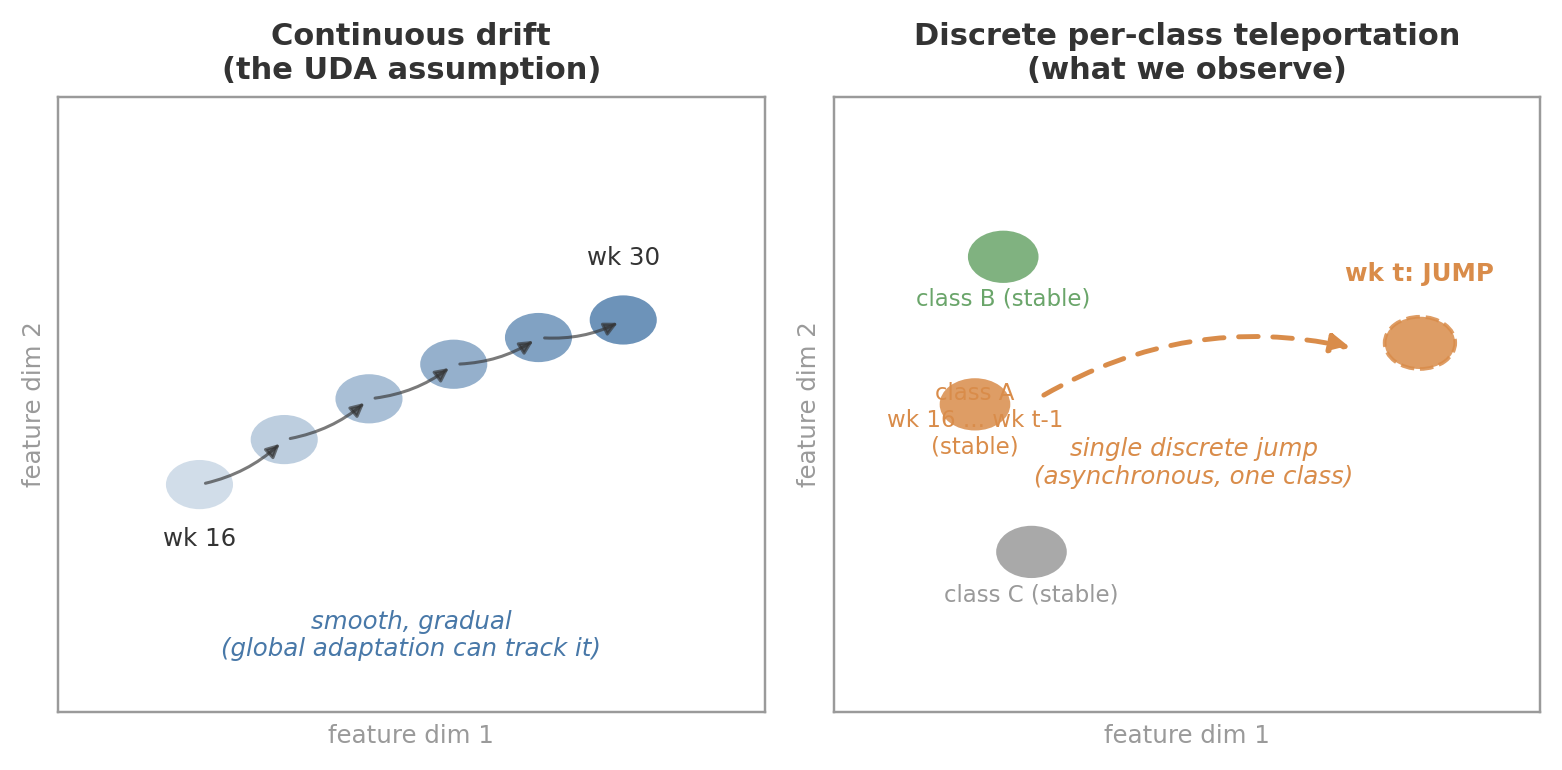
\includegraphics[width=\columnwidth]{figs/fig_continuous_vs_discrete_drift.png}}
\caption{\textbf{Continuous vs.\ discrete distribution shift (schematic).} Color encodes
deployment time ($\bigcirc$ first week $\to$ $\square$ last week). \emph{Left:} the
gradual, homogeneous drift that global UDA/CTTA assume --- within-week spread exceeds the
week-to-week centroid step, so a class smears along a single traceable path and a nearby
adaptation target always exists. \emph{Right:} the regime we document for encrypted traffic
--- each application stays put, then \emph{teleports} across empty latent space at its own
time (asynchronous), while the stable majority (grey) never moves. Blind global adaptation
chases the few jumpers and warps the stable majority. \TODO{caption prose final pass.}}
\label{fig:concept}
\end{figure}

\begin{figure}[htbp]
    \centering
    \begin{minipage}{0.48\linewidth}\centering
        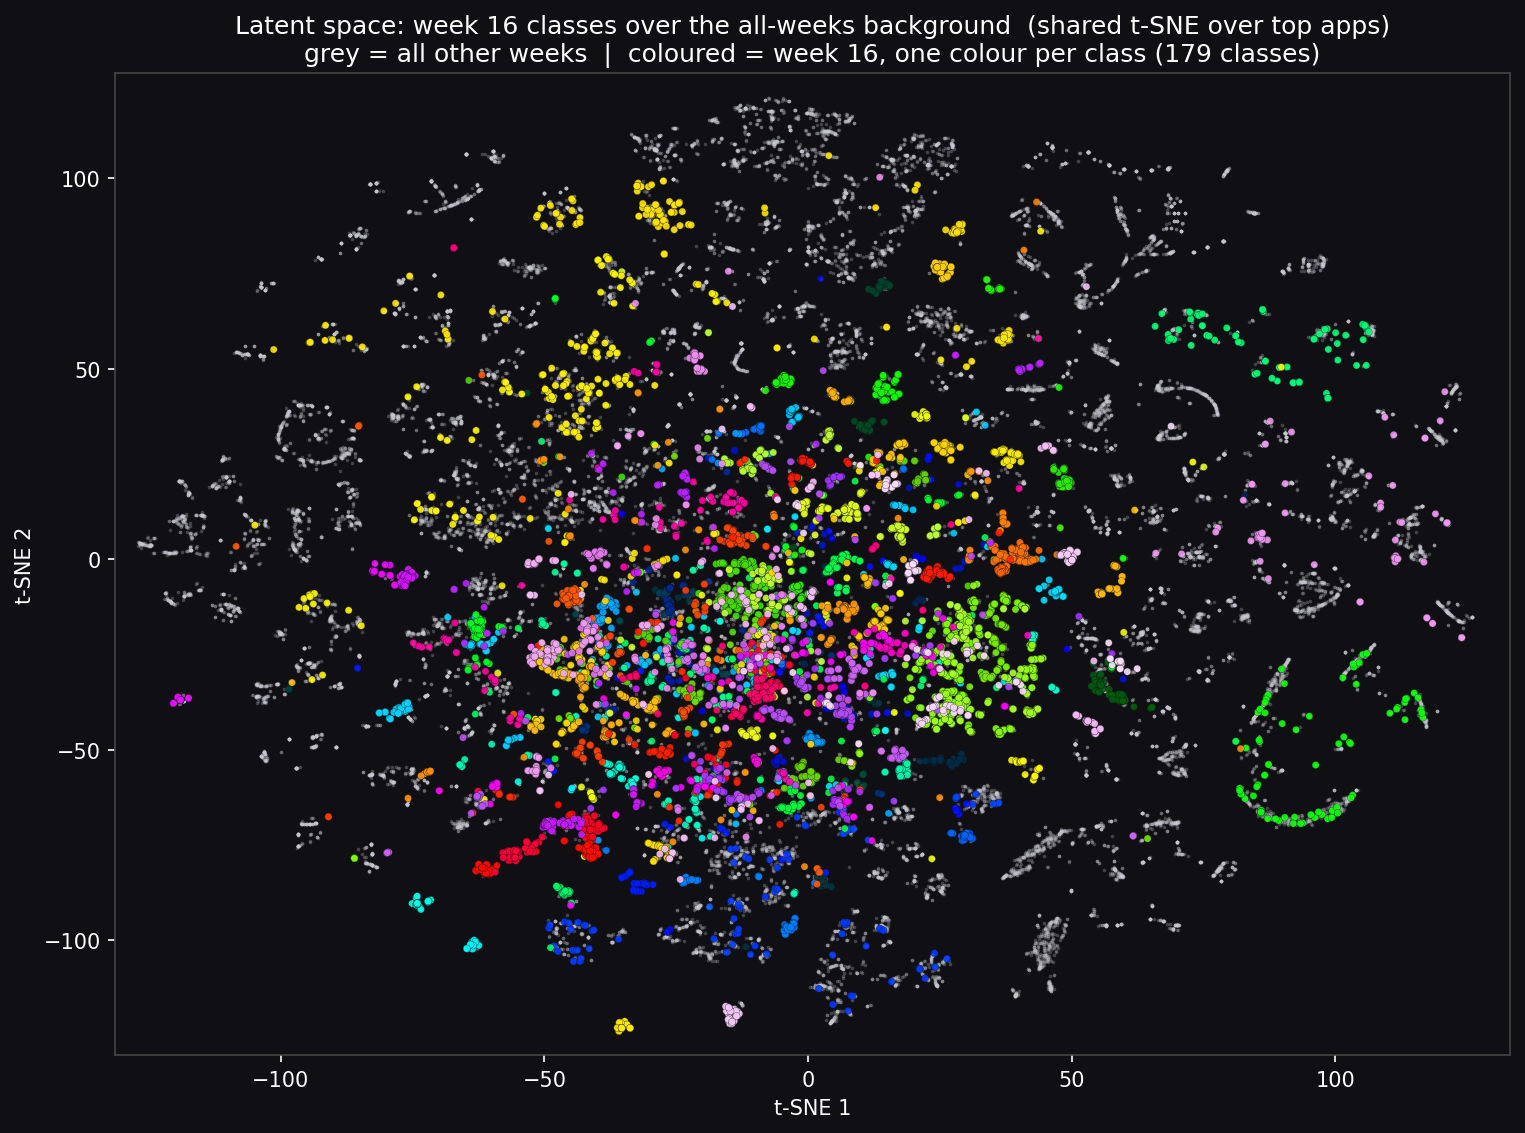
\includegraphics[width=\linewidth]{figs/tsne_background_w16_16to52_week16_byclass.png}
        \caption*{(a) Pristine class topology (Week-16 baseline)}
    \end{minipage}\hfill
    \begin{minipage}{0.48\linewidth}\centering
        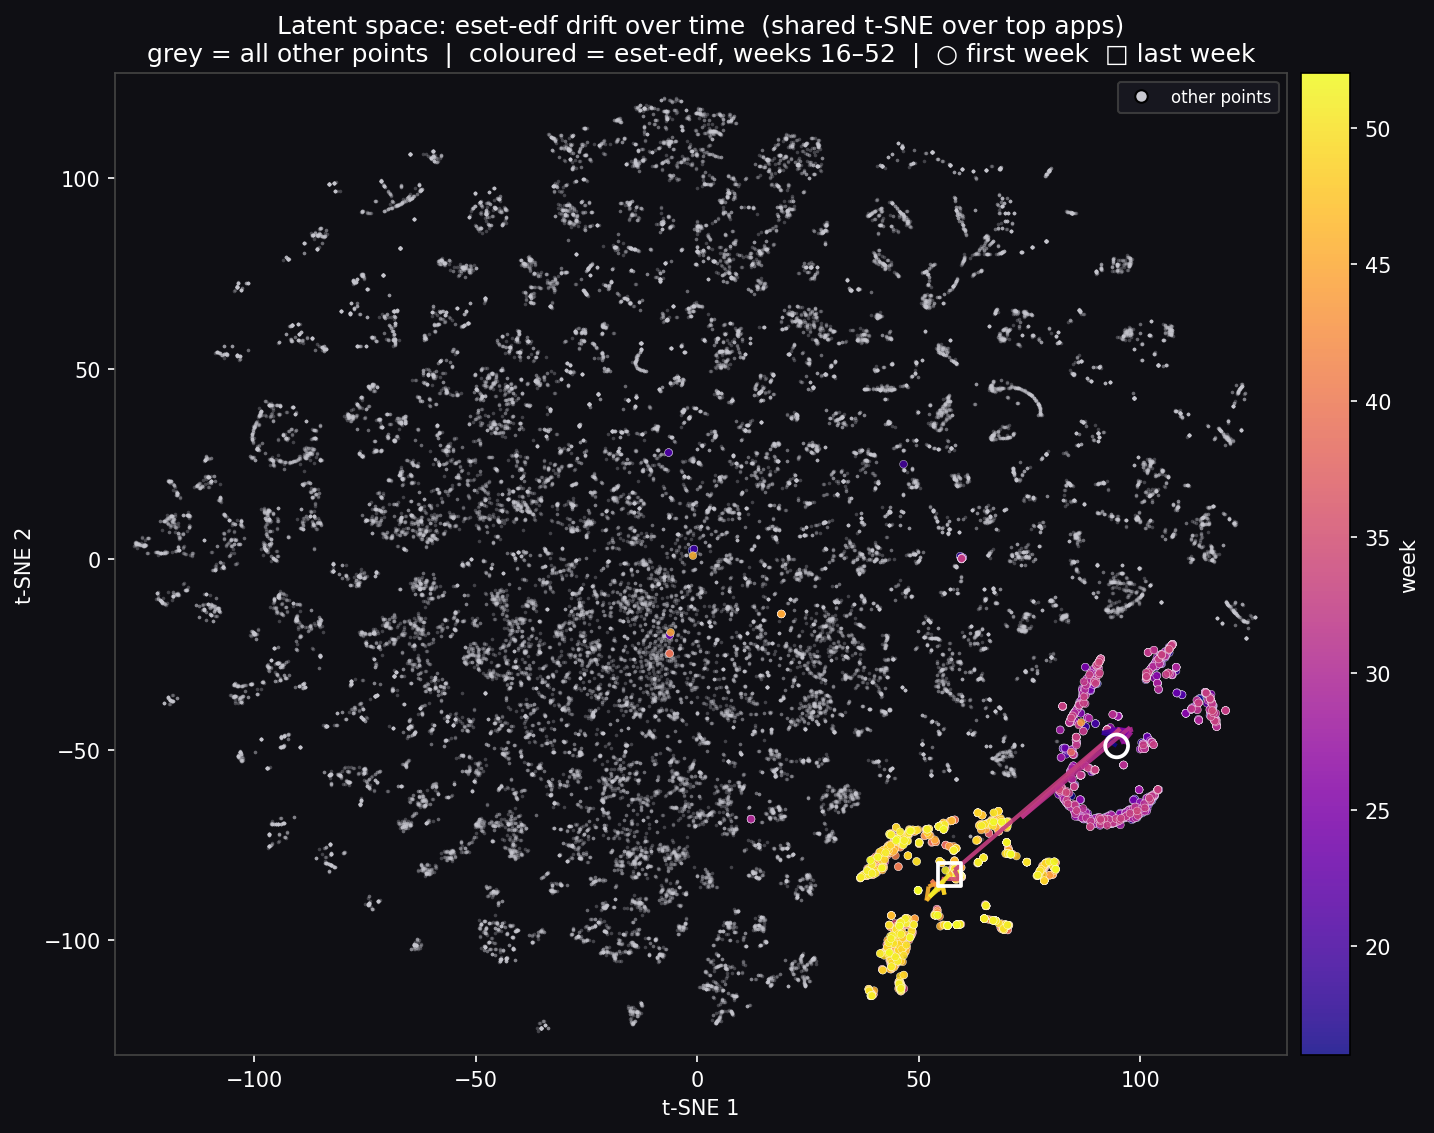
\includegraphics[width=\linewidth]{figs/tsne_temporal_w16_16to52_056_eset-edf.png}
        \caption*{(b) eset-edf (teleportation $\approx$ Week 34)}
    \end{minipage}
    \vspace{0.25cm}
    \begin{minipage}{0.48\linewidth}\centering
        
\includegraphics[width=\linewidth]{figs/tsne_temporal_w16_16to52_049_docker-registry.png}
        \caption*{(c) docker-registry (teleportation $\approx$ Week 27)}
    \end{minipage}\hfill
    \begin{minipage}{0.48\linewidth}\centering
        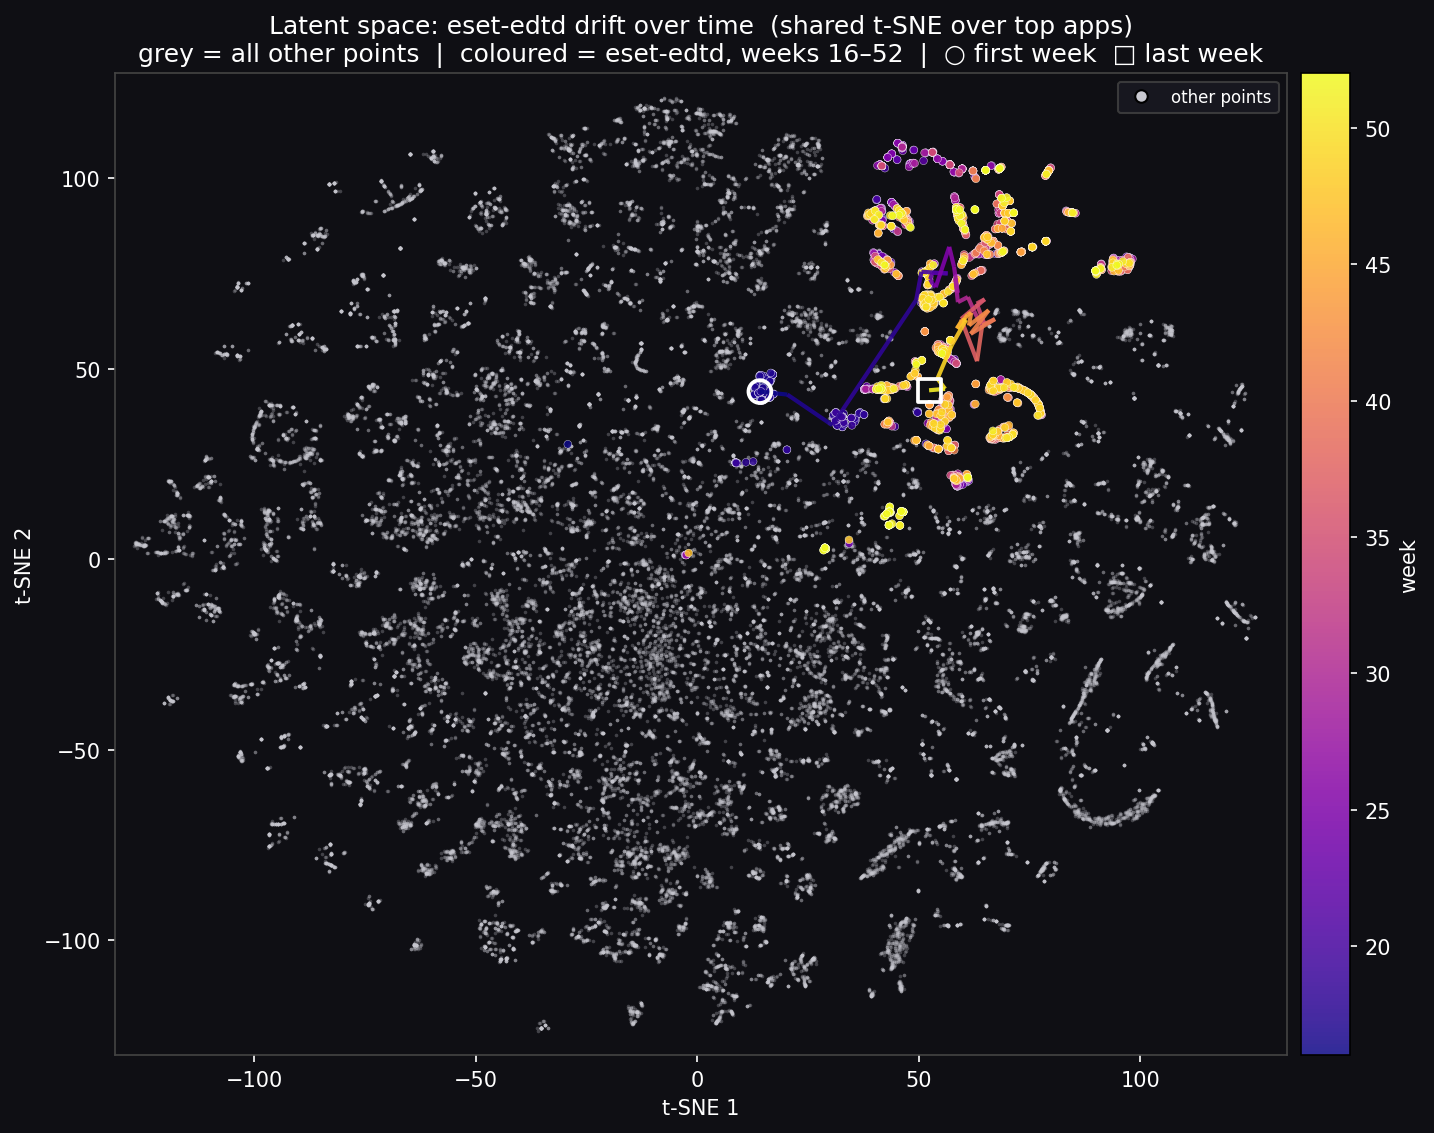
\includegraphics[width=\linewidth]{figs/tsne_temporal_w16_16to52_057_eset-edtd.png}
        \caption*{(d) eset-edtd (teleportation $\approx$ Week 17)}
    \end{minipage}
    \caption{\textbf{The Continuous Drift Fallacy} (Week-16 reference). Three
    applications that each held a stable signature for months and then teleported
    across empty latent space at \emph{different} times (eset-edtd $\approx$Week 17;
    eset-edf $\approx$Week 34; docker-registry $\approx$Week 27), against the
    pristine Week-16 topology (a). The stable majority never moves.}
    \label{fig:hero}
\end{figure}

Modern encrypted-traffic classification (ETC) is a behavioral discipline by
necessity. As TLS~1.3 and the Encrypted ClientHello (ECH) extension close the
last cleartext handshake fields that classic deep-packet inspection relied on,
operators are forced onto side-channel models that learn from packet timing,
direction, and size sequences rather than from payload content
\cite{shamsimukhametov2024ech,lin2022etbert,luxemburk2023tls,seddigh2019framework}. These models
report near-perfect accuracy in the lab, yet a well-documented lab-to-production
rift erodes that performance once they are deployed against live, evolving
traffic --- the same temporal-bias and realism gap (concept drift,
network-condition variation, label scarcity) that has been flagged across
malware and encrypted-traffic analysis more broadly
\cite{pendlebury2019tesseract,bahramali2023netclr}. The prevailing response is
to treat this erosion as a slow, global concept drift and to counter it with
unsupervised domain adaptation (UDA) or continual test-time adaptation (CTTA),
methods that assume the class boundaries move together, gradually, and in the
same direction.

We argue that this picture is wrong, and that getting it wrong is the reason
adaptation backfires. The literature documents at least three distinct failure
modes --- slow accuracy decay \cite{malekghaini2022data,jancicka2024noms},
abrupt collapses triggered by backend or version updates \cite{chen2025drift},
and outright generalization failures \cite{shamsimukhametov2024ech} --- but
treats them as points on a single continuous-drift spectrum. We call this the
\emph{Continuous Drift Fallacy} (Fig.~\ref{fig:concept}): the smooth macroscopic
accuracy decay that motivates global adaptation is not a coherent drift of the
whole feature space but a \emph{superposition} of discrete, asynchronous,
per-class steps. Individual applications hold their learned signature for many
weeks and then \emph{teleport} across empty latent space at their own,
vendor-driven moment (Fig.~\ref{fig:hero}, Fig.~\ref{fig:density}), while the
stable majority of classes never move. A method that updates the model globally
must chase the few jumpers, and in doing so it warps the decision geometry of
the many classes that were never broken --- the mechanism behind the negative
transfer we measure in Sec.~\ref{sec:negtransfer}.

This observation lets us reframe the problem. If the deployed model is held
\emph{frozen}, a class that teleports does not become a new class; it becomes a
\emph{known} class whose flows now fall outside the model's learned decision
region. Monitoring drift on a frozen model is therefore closer to inference-time
open-set detection of known-but-drifted classes than to domain adaptation
\cite{bendale2016openmax}. The operational stakes favor this view: as ECH
deployment broadens and the per-class breaks keep arriving asynchronously, a
full supervised retrain at every event is prohibitive --- it pays a fresh
labeling campaign across the whole service catalogue and risks re-incurring the
negative transfer above. The pragmatic loop is to identify \emph{which} classes
jumped, recapture samples for only those classes, and apply a targeted update.
A label-free per-class monitor is exactly what makes that loop actionable.

We study these effects on CESNET-TLS-Year22 \cite{hynek2024cesnet}, a
year-spanning backbone dataset, and contribute the following:
\begin{enumerate}[leftmargin=1.4em]
  \item We decompose the smooth macroscopic accuracy decay into one documented
        measurement-sensor step plus a long tail of asynchronous, per-class
        teleportations, and show the latter is covariate- rather than
        label-driven (Sec.~\ref{sec:discrete}).
  \item We show empirically that global adaptation is mis-specified for this
        regime: gradient CTTA induces negative transfer and best-case adversarial
        UDA buys no forward benefit (Sec.~\ref{sec:negtransfer}).
  \item We introduce a BBSE-corrected entropy residual --- a label-free,
        label-shift-robust per-class monitor that tracks hidden degradation and
        says \emph{which} class broke (Sec.~\ref{sec:method}--\ref{sec:eval}).
  \item We recast monitoring under an open-set lens and demonstrate a per-class
        diagnose-and-repair loop that restores broken classes without disturbing
        the stable majority (Sec.~\ref{sec:operational}).
\end{enumerate}

\begin{figure}[htbp]
\centerline{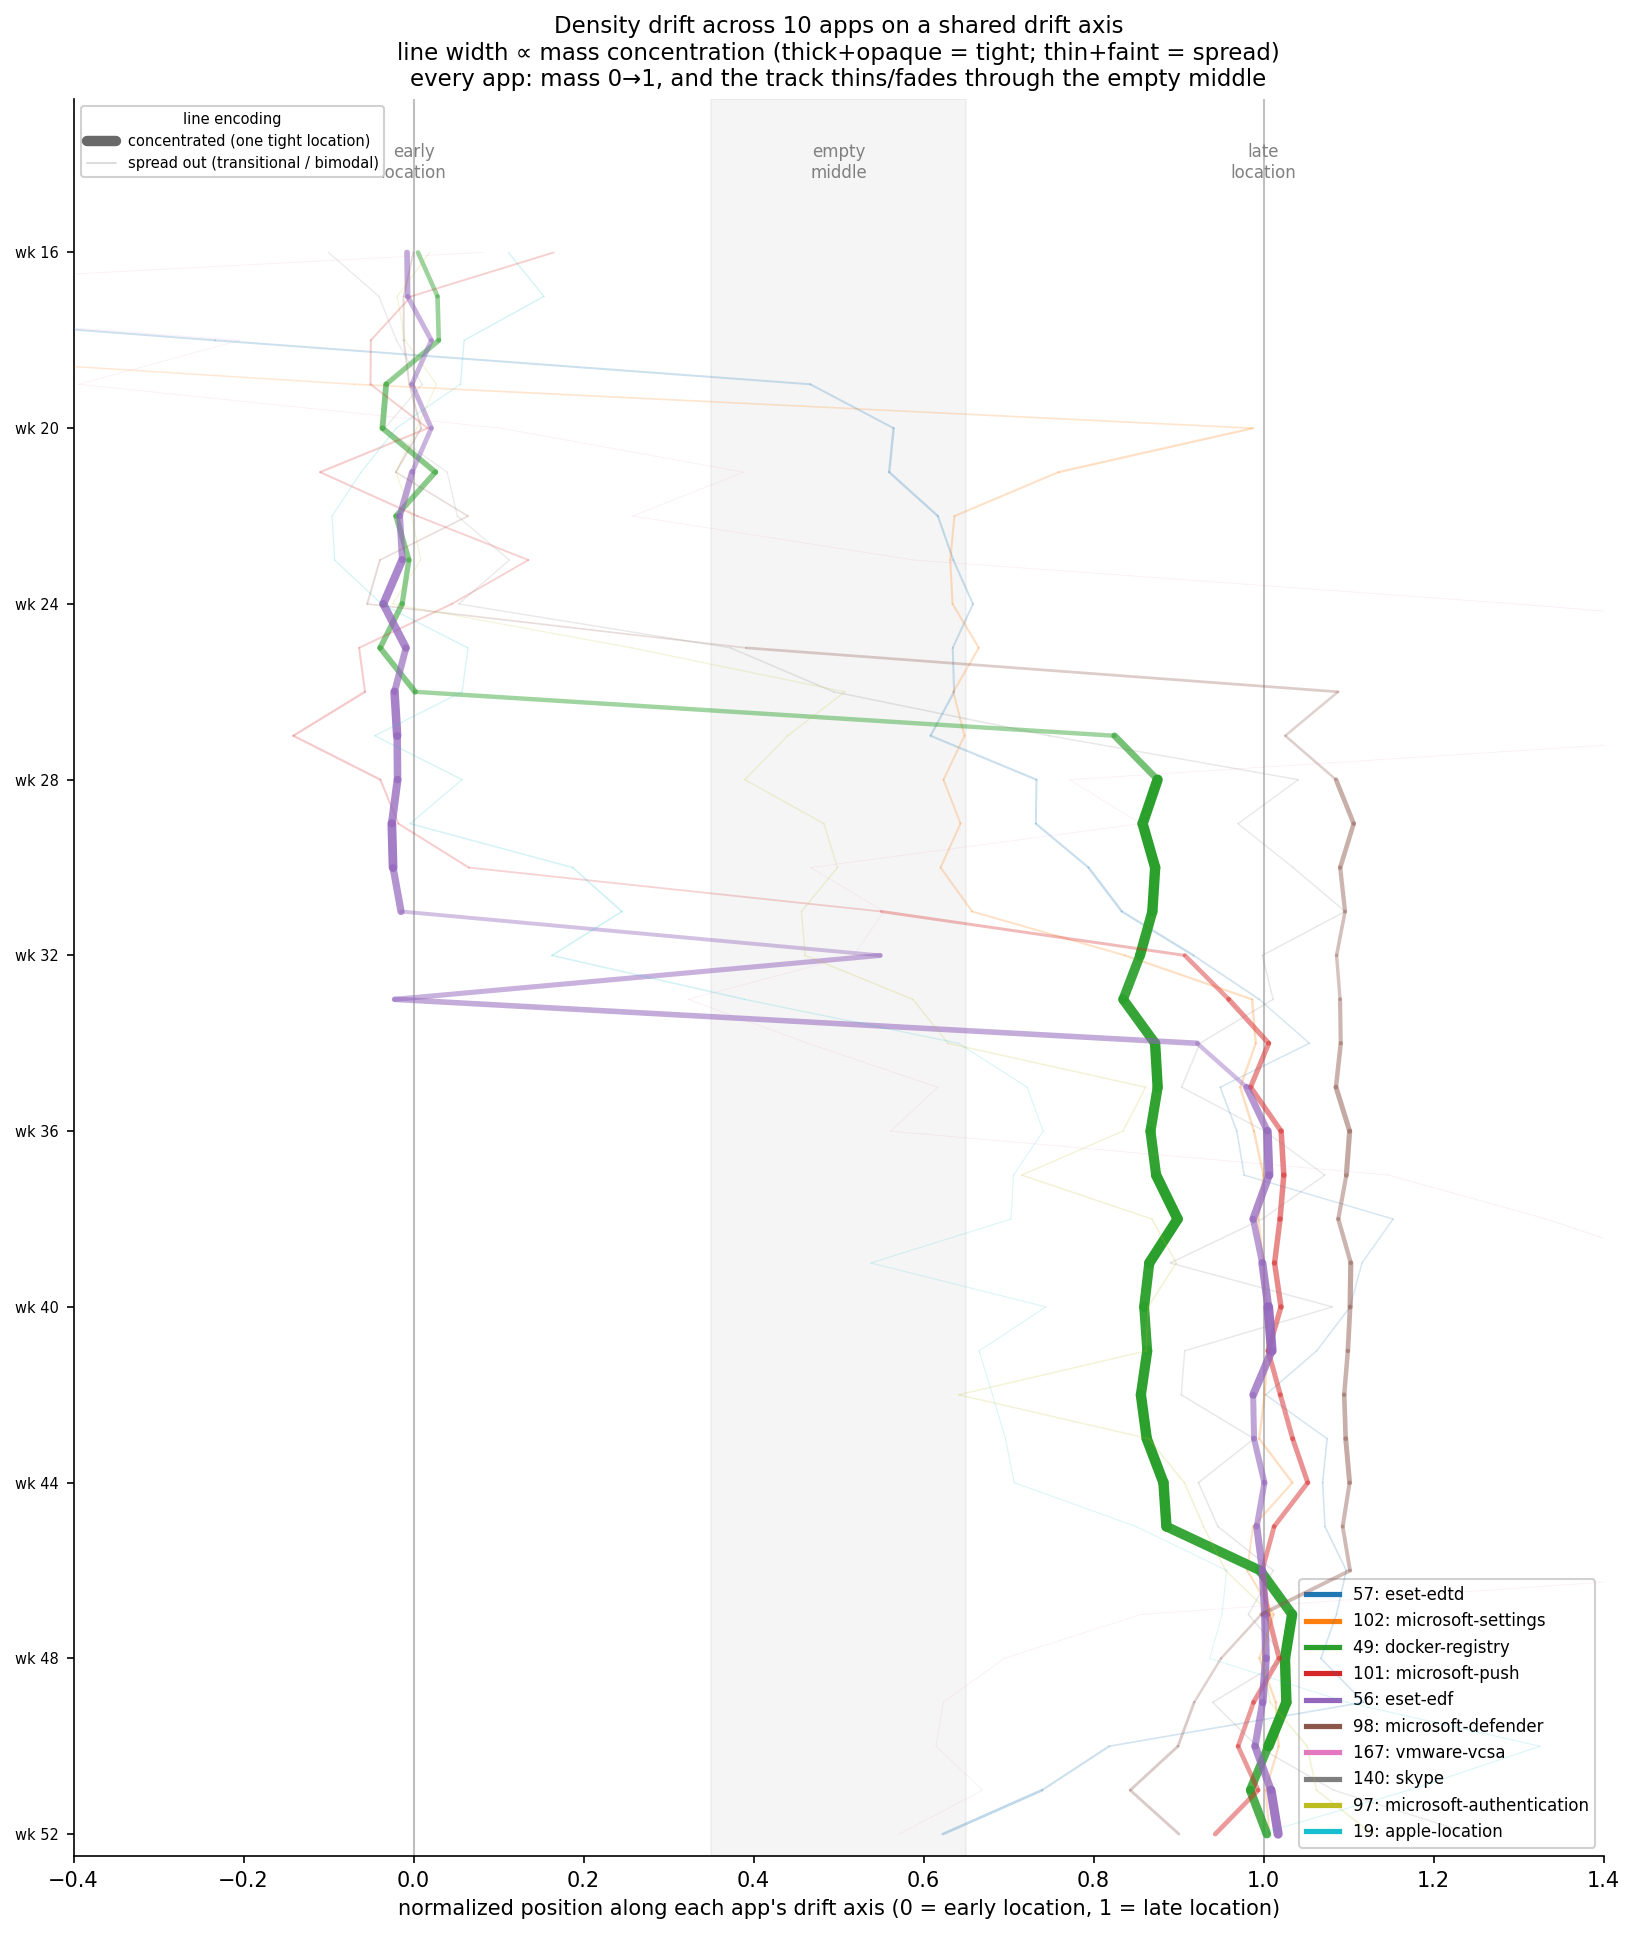
\includegraphics[width=\columnwidth]{figs/density_drift_multi_conc_w16_16to52_10apps.png}}
\caption{Continuous Drift Fallacy across 10 apps from Week 16 (asynchronous,
class-isolated jumps; thick=low-entropy/centered). \TODO{caption later.}}
\label{fig:density}
\end{figure}

%  OPTIONAL (parked per scope decision; cheap to generate from existing data):
%  the literal "smooth macro decay" curve = each week's own model (in-dist
%  diagonal) vs the frozen Week-1 model evaluated forward. Could anchor Sec III.
%  \begin{figure}[htbp]\centerline{\includegraphics[width=\columnwidth]{figs/fig_temporal_degradation_curve.png}}
%  \caption{Per-week vanilla (in-distribution) vs. frozen source-model decay.}\label{fig:macrocurve}\end{figure}

%==============================================================================
\section{Related Work}
\label{sec:related}

\subsection{Test-Time Adaptation and UDA}
The canonical responses to distribution shift in deployed models are
entropy-based test-time adaptation (TENT \cite{wang2020tent}), its continual
variant with consistency and stochastic restoration (CoTTA \cite{wang2022cotta}),
and domain-adversarial feature alignment (DANN \cite{ganin2016dann}). What unites
these methods is that they are \emph{global}: they update shared parameters (BN
affine terms, all weights, or the feature extractor) to align the entire
target distribution to the source. This is the right move when class boundaries
drift cohesively, but it is mis-specified for local, asynchronous drift, where
only a handful of classes have moved. A global update driven by the aggregate
target statistics then warps the decision geometry of the stable majority,
producing negative transfer rather than recovery. Compounding the problem, TTA
and CTTA are rarely evaluated on encrypted traffic at all, so their behavior in
this regime is largely undocumented. We supply that benchmark in
Sec.~\ref{sec:negtransfer}.

\subsection{Unsupervised Drift Monitoring Frameworks}
The closest prior art is MFWDD \cite{mfwdd2024}, a model-based feature-weight
drift detector demonstrated on TLS and QUIC traffic, together with the recent
CESNET dataset-stability benchmark \cite{cesnetdrift2025}. Two contrasts
motivate our work. First, MFWDD's label-free mode is a \emph{global} trigger
that attributes drift to \emph{features}, not classes; per-class attribution in
that framework requires labels. Second, the feature-distribution distances such
detectors rely on also move under \emph{benign} label shift --- a viral volume
spike on one application shifts the marginal feature distribution without any
loss of accuracy --- so a feature-distance trigger cannot tell a structural break
from a benign surge. Our signal is instead per-class, label-free,
\emph{label-shift-corrected}, and calibrated against hidden $F_1$; we benchmark
it head-to-head against an MFWDD-style global detector in
Sec.~\ref{sec:robustness} and Sec.~\ref{sec:isolation}. We see the two as
complementary rather than competing: MFWDD answers \emph{which feature drifted}
(useful for dataset curation), whereas our monitor answers \emph{which class
broke} (the input to a targeted repair). Adjacent encrypted-traffic work on
website and mobile-app fingerprinting has independently encountered drift but
stays robustness-oriented --- seeking drift-invariant representations
\cite{jiang2022fgnet}, augmentation- and realism-robust training
\cite{bahramali2023netclr}, or treating per-website change as a targeted
per-classifier update rather than a holistic retrain \cite{deng2023ares}. None
provides a label-free monitor that localizes which class broke, which is the
niche we occupy.

\subsection{Label-Shift Quantification}
Our monitor builds on the label-shift estimation literature: Black Box Shift
Estimation (BBSE) \cite{lipton2018bbse}, the EM-style prior-adjustment of
Saerens \emph{et al.} (SLD-EM) \cite{saerens2002sld}, regularized learning under
label shift (RLLS) \cite{azizzadenesheli2019rlls}, the unified
maximum-likelihood view (MLLS) \cite{garg2020mlls}, its bias-corrected
calibrated variant (MLLS+BCTS) \cite{alexandari2020mlls}, and Bayesian black-box
quantification \cite{ziegler2023bayesian}. Crucially, every one of these
estimators rests on the same assumption that the class-conditional $P(X\mid Y)$
is invariant between source and target. A covariate shift violates that
assumption and breaks all of them \emph{together}. Where the label-shift
literature treats this as the failure case to avoid, we \emph{weaponize} it: the
shared breakdown is precisely the signal that distinguishes a genuine structural
break from a benign change in class proportions. Online label shift, which
corrects a drifting $P(y)$ under fixed $P(x\mid y)$, is the mirror image of our
setting and we discuss it only as contrast and future work
(Sec.~\ref{sec:conclusion}).

\subsection{Open-Set Recognition and the Monitoring Lens}
\label{sec:related_osr}
Open-set recognition (OSR) equips a classifier to reject inputs that fall
outside its learned decision regions \cite{bendale2016openmax}. We borrow this
\emph{lens}, not its algorithms. When a deployed model is held frozen, a known
class that teleports falls outside the decision geometry the model learned for
it, so at inference those flows behave like out-of-region or ``unknown''
samples. Drift monitoring on a frozen model is therefore well described as
inference-time open-set detection. We stress the distinction from the usual OSR
problem: these are \emph{known} classes whose signatures drifted, not
\emph{novel} classes appearing for the first time. We consequently adopt the
open-set view of a per-class decision region as an interpretive frame and do not
claim an OSR algorithmic contribution. For the same reason we do not run an OSR
baseline battery in the main monitoring evaluation --- our detector is scored
against hidden $F_1$ and compared against MFWDD-style and uncorrected-entropy
detectors --- though we do report a per-class energy/MSP out-of-distribution
comparison in Sec.~\ref{sec:robustness} to address the natural ``why not OOD
methods'' question directly. The closest cousin to our framing is HOLMES
\cite{deng2024holmes}, which already instantiates the per-class open-set view in
encrypted traffic with spatial decision regions, out-of-region rejection, and
even per-class region updates on drift. HOLMES, however, is supervised --- labels
define its regions --- and is a website-fingerprinting \emph{attack}; our monitor
is label-free, operates on a frozen ETC model, and additionally quantifies the
harm of global adaptation. We borrow the lens, not the algorithm.

%==============================================================================
\section{The Nature of Discrete Drift in Encrypted Traffic}
\label{sec:discrete}

\subsection{Two Modalities of Discrete Drift}
\label{sec:modalities}
We study CESNET-TLS-Year22 \cite{hynek2024cesnet}, a year-spanning 2022 dataset
of TLS flows from a 100\,Gbps backbone, organized as 52 weekly snapshots
covering 180 services across 24 categories. Our backbone is the multimodal
mm-CESNET architecture --- a Conv1D branch over the per-packet (PPI) sequence
plus an MLP over flow statistics --- taken from the open-source cesnet-models
codebase \cite{luxemburk2023tls}. No source weights are released for this
dataset, so we train every source model ourselves.\footnote{The 96.3\%
next-week ($T{+}1$) accuracy reported for this dataset \cite{hynek2024cesnet} is
measured under the authors' own protocol; our numbers are 52-week
\emph{forward} averages of a frozen model under accumulating drift and are not
comparable to it. The like-for-like reference is our own in-distribution
accuracy, 0.845 at Week-1 and 0.883 at Week-16.}

The macroscopic accuracy curve of a frozen source model decaying over the year
looks like continuous drift, but it resolves into two qualitatively different
modalities. \textbf{Modality~1} is a single documented measurement-infrastructure
event at Week~10: a 9~March~2022 ipfixprobe exporter upgrade that began skipping
retransmitted packets, coinciding with post-invasion DDoS conditions
\cite{hynek2024cesnet}. This is not application drift but a sensor change, and we
repurpose it as a \emph{ground-truth} covariate event; MFWDD independently
flagged the same period, triggering two of its retrainings and attributing them
to the monitoring change \cite{mfwdd2024}. \textbf{Modality~2} is the asynchronous
application \emph{teleportation} that dominates from Week~16 onward: genuine,
vendor-driven, per-class step changes in which one application's signature jumps
across empty latent space while its neighbors stay put
(Figs.~\ref{fig:hero},~\ref{fig:density}). This is not a CESNET-specific artifact
--- per-application version updates are known to drive per-class signature shifts
in mobile-app fingerprinting \cite{jiang2022fgnet}, and the same teleportation
reproduces on an independent, proprietary closed-world dataset (anonymized for
review; Sec.~\ref{sec:negtransfer}, Appendix
Fig.~\ref{fig:app_proprietary_tsne}).

A natural objection is that the vulnerable classes are simply long-tail and
under-trained. The \emph{timing} of their collapse rules this out. The
vulnerable classes hold their accuracy for many weeks and then step-drop at
\emph{different} weeks (Fig.~\ref{fig:classdrop}): an under-trained class would
be weak from Week~1, not fall sharply at Week~28. We therefore avoid a static
$F_1$-versus-frequency scatter, which would merely re-assert the scarcity
confound we are dispelling, and rely on the timed step-drop signature instead.

We apply one reference-week rule throughout, which also settles the
Week-1-versus-Week-16 question. Week-16 is the clean-regime reference for all
Modality-2 analyses (it is healthy, with Macro-$F_1\geq0.76$ across weeks 13--20
and a 0.806 peak at Week-16); Week-1 is used to expose and validate
the documented Week-10 event (Modality~1) and---because it alone carries the
healthy-versus-degraded week split---to anchor the primary anomaly-detection
benchmark, which we replicate on Week-16 (Sec.~\ref{sec:robustness}). The conclusion is that the smooth
macro curve is a one-time sensor step plus a long tail of asynchronous per-class
steps, not continuous drift.

%  TRAINING-FREQUENCY FIGURE REMOVED FROM BODY (cut-candidate; see Appendix
%  Fig.~\ref{fig:app_trainfreq}). Reason: a static F1-vs-frequency scatter
%  introduces a data-scarcity confound that competes with the teleportation
%  thesis; the long-tail point is now made safely in prose above.

\begin{figure}[htbp]
% NEW (v12): Week-16 per-class recall@1 over time. Direct evidence for asynchronous,
% timed step-drops (the Modality-2 signature). Recall-only view; the BBSE-proportion
% decoupling is shown separately by Fig.~\ref{fig:grid} in Sec.~\ref{sec:mirror}.
\centerline{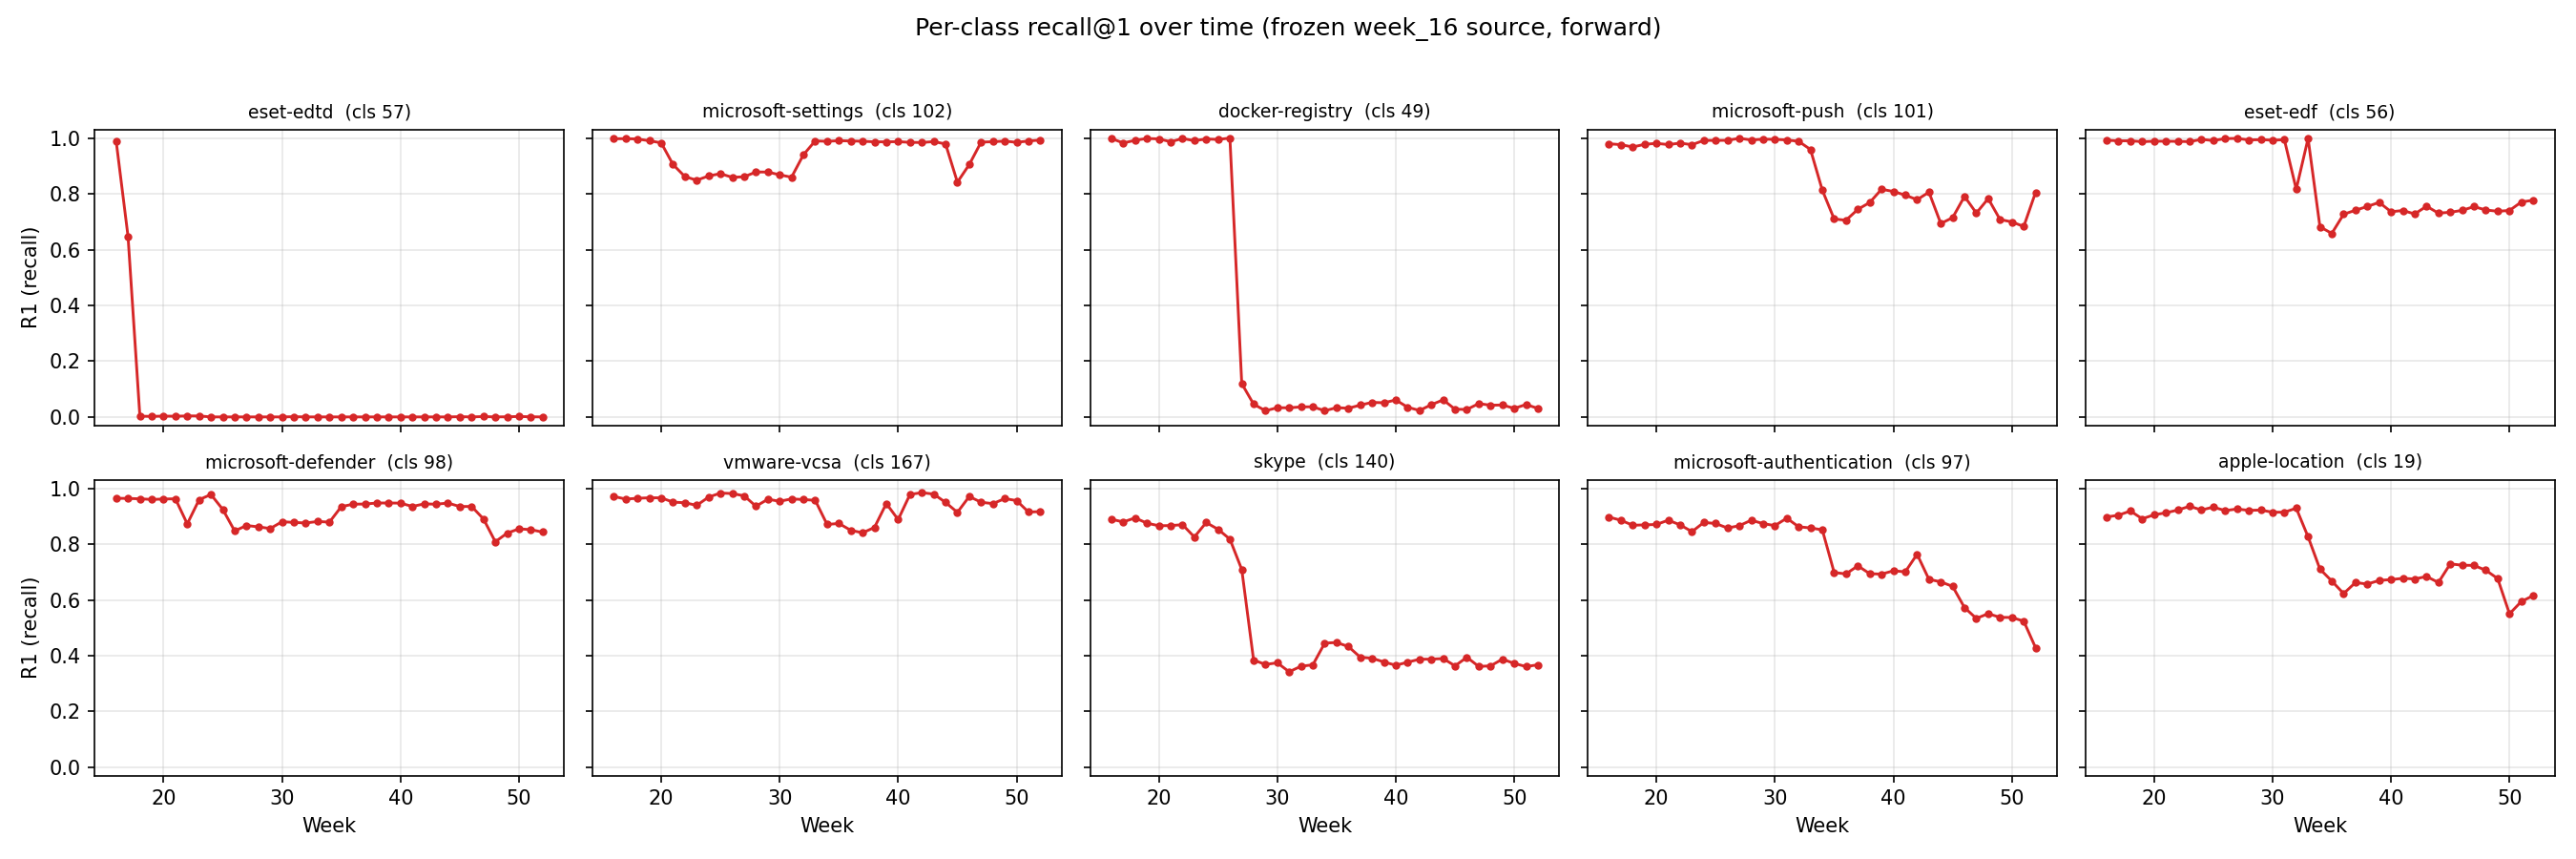
\includegraphics[width=\columnwidth]{figs/fig_class_drop_w16_selected_grid.png}}
\caption{Per-class recall@1 over time (frozen Week-16 source, forward). Top classes
hold for many weeks then collapse in isolated step functions at \emph{different} times
(e.g.\ eset-edtd $\approx$wk17, docker-registry $\approx$wk28, skype $\approx$wk28),
the per-application signature of asynchronous teleportation -- not a uniform decay.
\TODO{caption later.}}
\label{fig:classdrop}
\end{figure}

\subsection{Decomposing Performance Degradation}
\label{sec:decompose}
To attribute the degradation to its source, we run a synthetic ablation that
separates label shift from covariate shift \cite{lipton2018bbse,saerens2002sld}.
A \emph{synthetic-$F_1$} curve resamples the reference-week features to match each
week-$t$'s label proportions, isolating the effect of pure \emph{label} shift; a
\emph{corrected-$F_1$} curve evaluates on the genuine week-$t$ features but forces
the reference label proportions, isolating the effect of pure \emph{covariate}
shift. We run this with both references, for the two distinct purposes the
reference-week rule prescribes. Under the Week-1 reference
(Fig.~\ref{fig:decomp_w1}), the Week-10 step crash is driven almost entirely by
covariate shift while synthetic label shift stays benign, confirming the
documented sensor cause of Modality~1. Under the Week-16 reference
(Fig.~\ref{fig:decomp_w16}), the clean-regime teleportation degradation across
weeks 17--52 is \emph{also} covariate-driven, with the label-shift-only curve
holding at the 0.806 baseline. The second panel closes the ``you only validated
the sensor break'' gap: the asynchronous per-class teleportations of Modality~2
are a covariate phenomenon too, not a benign reshuffling of class volumes.

\begin{figure}[htbp]
\centerline{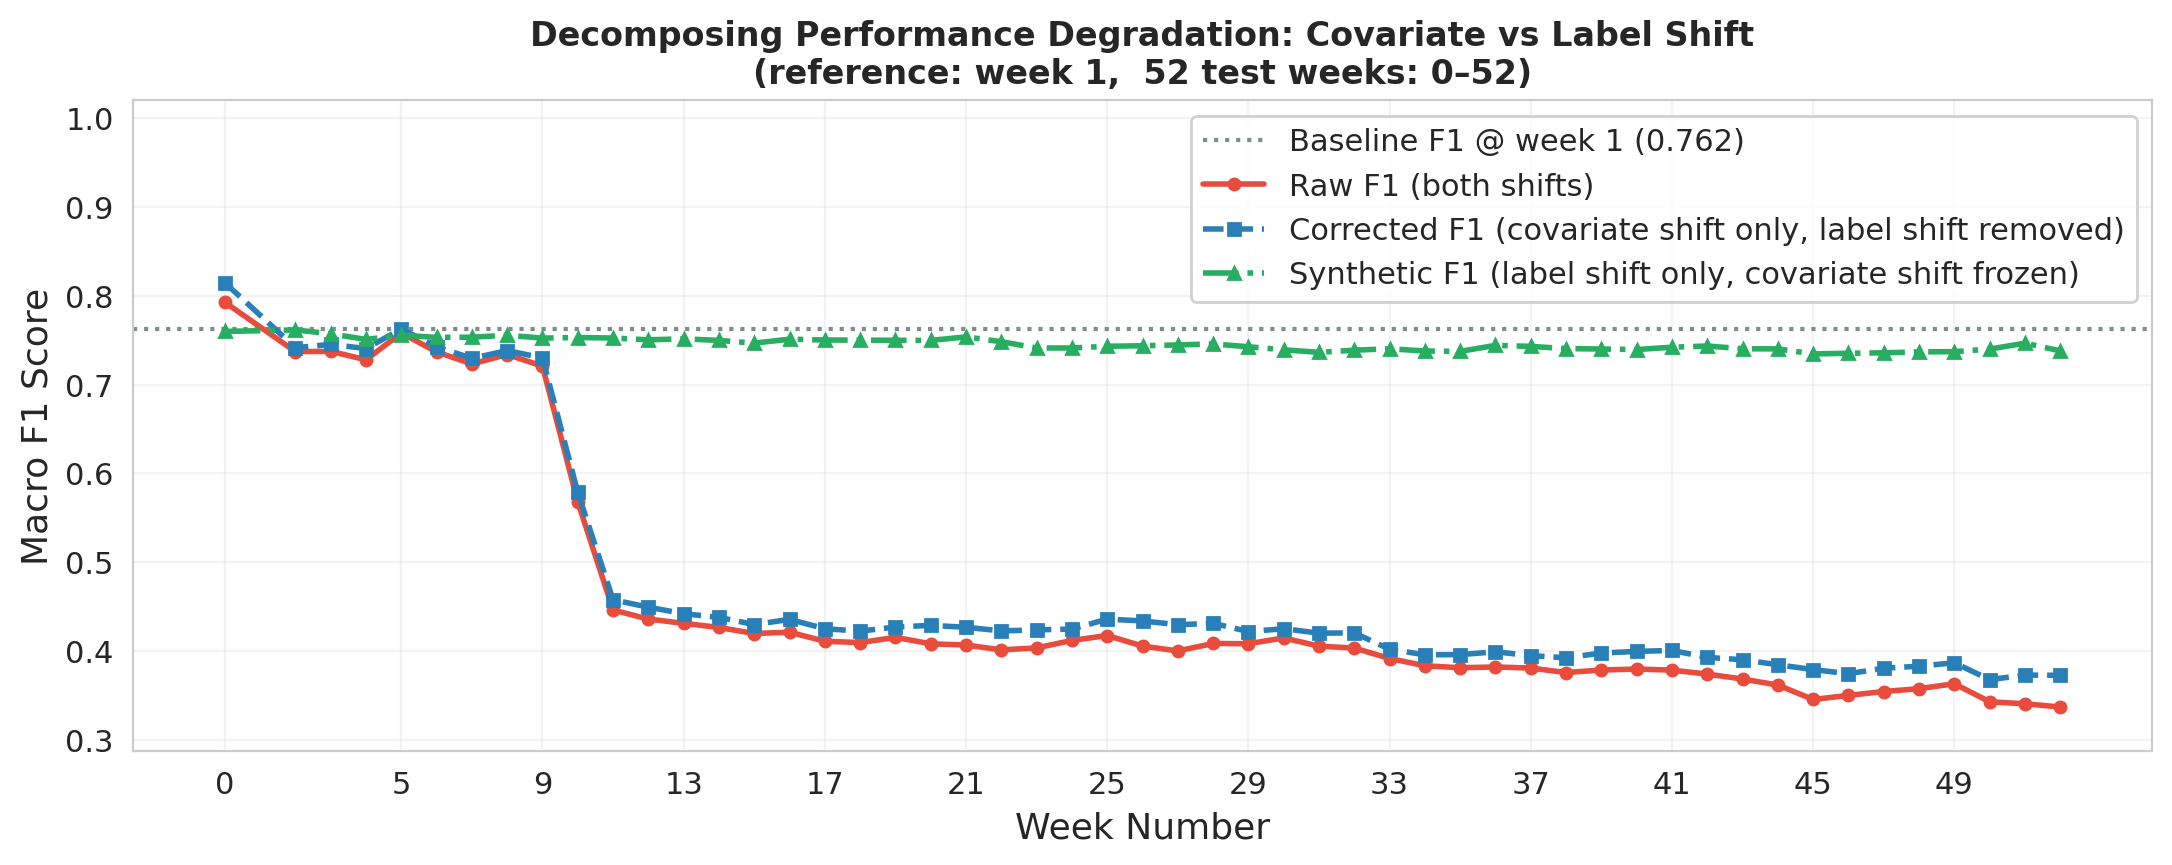
\includegraphics[width=\columnwidth]{figs/fig_combined_penalties (1).png}}
\caption{Decomposition, Week-1 reference: the Week-10 step crash is driven by
COVARIATE shift; synthetic label shift is benign (validates the documented
sensor-induced change). \TODO{caption later.}}
\label{fig:decomp_w1}
\end{figure}

\begin{figure}[htbp]
% NEW (author-added): Week-16 reference, test weeks 17-52. Save upload here.
\centerline{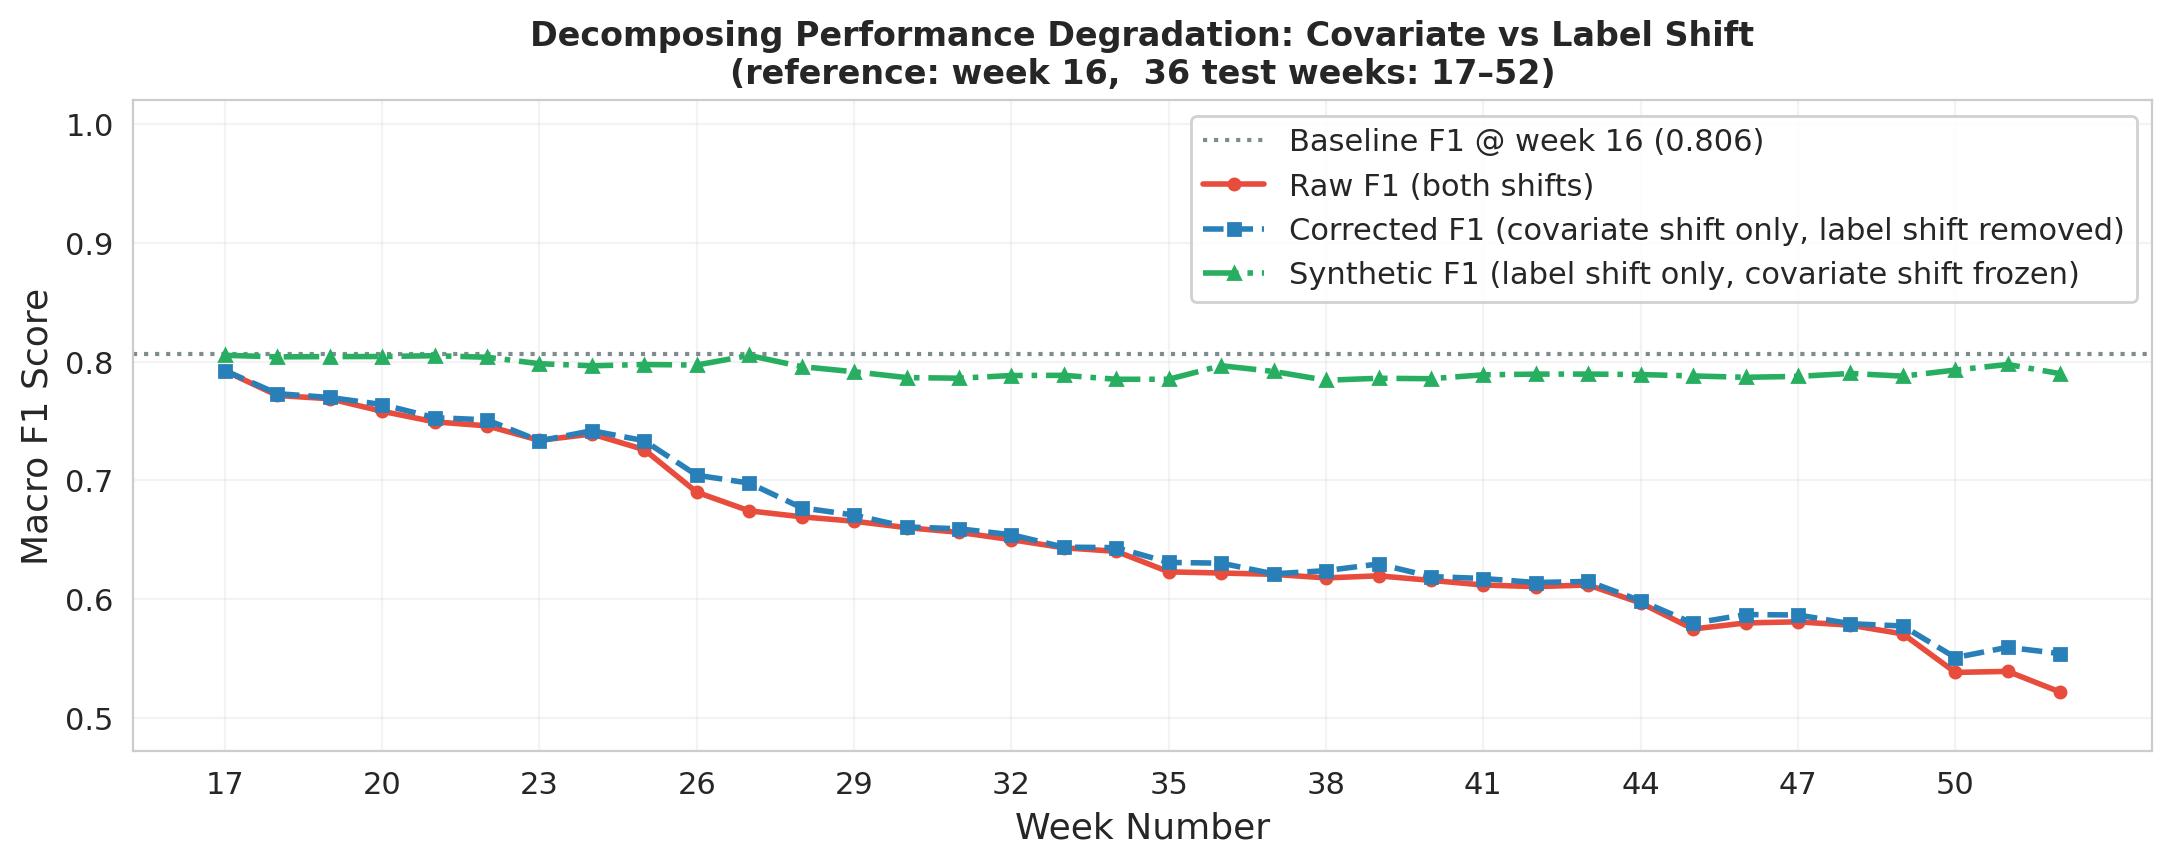
\includegraphics[width=\columnwidth]{figs/fig_combined_penalties_ref16.png}}
\caption{Decomposition, Week-16 reference (test weeks 17--52): degradation is COVARIATE-driven,
while label-shift-only (Synthetic) stays at the 0.806 baseline. \TODO{caption later.}}
\label{fig:decomp_w16}
\end{figure}

\subsection{Case Study: An Anchored Signature Shift (eset-edtd $\approx$wk17)}
\label{sec:casestudy}
We single out the eset-edtd service as a worked example because, unusually, it
carries a verifiable real-world anchor. Under the frozen Week-16 source, its
recall holds through the healthy regime and then collapses in a single step at
ISO week~17 (Fig.~\ref{fig:classdrop}); the same jump is visible in the latent
space (Fig.~\ref{fig:hero}d). The latent evidence is discrete rather than gradual:
the mean $L_2$ distance of week-$t$ eset-edtd embeddings from the Week-16 centroid
is flat across weeks 14--16 ($\approx5.3$) and then steps to $8.3$ at week~17 and
$12.9$ at week~18 --- a jump, not a ramp.

The anchor is dated. ESET \emph{Dynamic Threat Defense} (EDTD) was renamed to
\emph{ESET LiveGuard Advanced} on 27~April~2022 ($\approx$ISO week~17), a rebrand
that shipped backend, endpoint, and proxy-component changes --- a plausible
mechanism for a shift in the encrypted signature. We frame this honestly: the
match between the recall cliff and the rename is a strong timing coincidence with
a credible mechanism, not proven causation, and the encrypted traffic precludes
any payload-level confirmation.

To localize the shift inside the model, we attribute the latent drift back to the
raw inputs with SHAP \cite{lundberg2017shap} (Fig.~\ref{fig:shap}). We wrap the
frozen Week-16 encoder so that its scalar output is the embedding's distance from
the Week-16 centroid, then run a GradientExplainer over the PPI inter-packet-time,
direction, and size sequences plus the 44 flow statistics. The week-17 jump is
dominated by the PPI payload-\emph{size} sequence (mean$|$SHAP$|=4.38$), followed
by per-packet \emph{direction} ($1.50$) and inter-packet timing ($0.49$);
flowstats contribute only marginally. The drift therefore lives in the
packet-level size/direction signature, consistent with a changed handshake or
transport profile rather than a mere change in volume. A complementary check
agrees: a gradient-boosted domain classifier trained to separate the pre-cliff
(weeks 14--16) from the post-cliff (weeks 17--19) regime on interpretable
per-flow features reaches AUC~$0.92$, so the two periods are nearly linearly
distinguishable --- a discrete regime change --- and its top signed driver is
reverse-direction volume (BYTES\_REV falls $5578\!\to\!3551$), i.e.\ less
server-to-client payload after the cliff.

A second class, docker-registry, teleports at $\approx$Week~27 (well clear of the
Week-10 artifact) with the same signature: bulk-transfer features give way to
lighter, chattier signaling. We make no dated real-world claim for it --- the only
documented 2022 Docker event, the Hub v1 endpoint deprecation on 5~September~2022
($\approx$week~36), is some nine weeks late and is an API/authentication change
rather than a payload flip --- so it serves purely as an unattributed mechanistic
illustration of what a signature shift looks like in feature space. Together, an
anchored and dated per-class step (eset-edtd) and a mechanistically identical but
unattributed one (docker-registry) establish that teleportation is a real,
vendor-driven, per-application event that a frozen global model has no way to
anticipate.

\begin{figure}[htbp]
\centerline{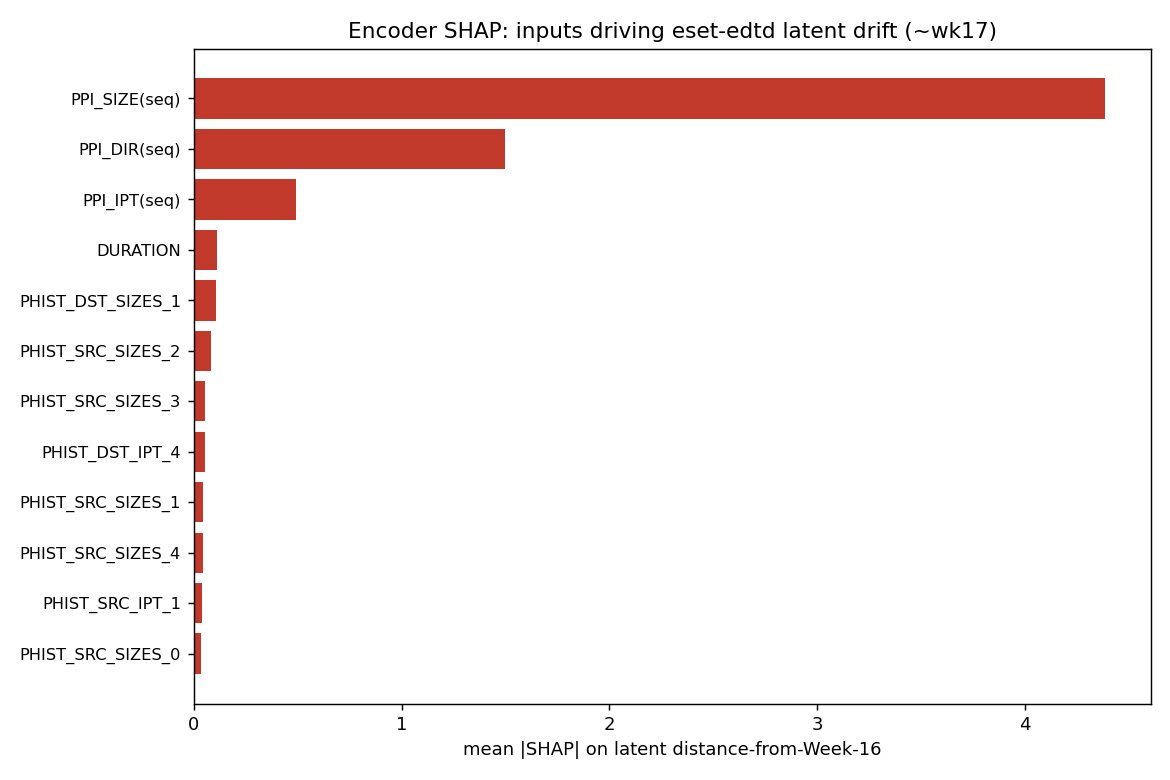
\includegraphics[width=\columnwidth]{figs/fig_shap_eset_edtd.png}}
\caption{Encoder SHAP \cite{lundberg2017shap} for eset-edtd: inputs driving the
frozen Week-16 latent drift at the $\approx$wk17 cliff (objective = embedding
distance from the Week-16 centroid). The shift is dominated by the PPI
payload-size sequence, then per-packet direction and inter-packet timing;
flowstats contribute marginally. This is feature \emph{attribution} of where the
model's representation moved, not a causal claim about the cause of the move.}
\label{fig:shap}
\end{figure}

%==============================================================================
\section{Why Global Adaptation Fails: Negative Transfer}
\label{sec:negtransfer}
%  PROMOTED to its own section (was Sec V-D). This is the empirical anti-UDA leg.
%  SELF-CONTAINED: uses only the frozen model + standard adapters, NOT our residual.

A reviewer who accepts that drift is per-class might still ask: why not adapt
globally anyway? We answer empirically. We take one source model, hold it frozen,
and evaluate it forward over every later week, comparing it against four standard
adapters: AdaBN \cite{li2016adabn}, which only recalibrates BN statistics and
performs no gradient update; TENT \cite{wang2020tent}, which updates the BN affine
parameters by entropy minimization; CoTTA \cite{wang2022cotta}, which updates all
parameters; and DANN \cite{ganin2016dann}, adversarial feature alignment. All
share the backbone, a 10\% sample, and seed~42, so any difference is attributable
to the adaptation mechanism. Because small batches inflate the BN-recalibration
effect, we report TENT and CoTTA at both batch~64 and batch~256, treating the
batch~256 (training-batch) figure as the fair operating point.

The results (Tables~\ref{tab:nt_tls1},~\ref{tab:nt_tls16},~\ref{tab:nt_quic}) tell
a consistent story. The gradient methods, TENT and CoTTA, are net-negative on
both TLS source weeks and on QUIC; because the failure spans the entropy- and
consistency-based families alike, the culprit is the global \emph{scope} of the
update, not any single algorithm. The damage is temporal: TENT and CoTTA fall
furthest on the far, drifted weeks --- exactly where adaptation is supposed to
help --- with batch~64 collapsing worst and even batch~256 remaining negative.
TENT's Macro-$F_1$ collapse at Week-1 ($0.362$ against the source's $0.455$) is the
signature of entropy minimization concentrating mass on the dominant classes
under label shift. The AdaBN control is the decisive comparison: with no gradient
step, BN-statistic recalibration alone induces no negative transfer forward-only
($|\Delta|\leq0.011$ on TLS --- $-0.009$ at Week-1, $-0.011$ at Week-16) and even a
small positive $+0.020$ on QUIC, exactly what the global-parameter-update thesis
predicts. (The apparent $+0.007$ AdaBN ``gain'' at Week-16 reported elsewhere is
backward transfer to the easy pre-source weeks and vanishes forward-only; see the
multi-seed significance table, Table~\ref{tab:nt_seedvar}.) The QUIC $+0.020$ is
fully consistent with the thesis precisely because it carries no parameter
update toward an adaptation objective: re-estimating statistics cannot harm the
stable majority. The harm, in short, is global parameter updates, not adaptation
per se.

DANN deserves separate treatment, because it is no longer harmful here --- it is
merely useless. Even in its most favorable per-target-week diagonal
(transductive) setting, where each week is scored by its own
source-16$\to$week-$N$ aligned model, DANN beats the frozen source by only
$+0.006$ on average ($+0.001$ on the far weeks; Table~\ref{tab:nt_dann}, per-week
in Fig.~\ref{fig:dann_curve}). Global source--target alignment buys no forward
robustness and cannot recover per-class discrete drift. All of these effects
reproduce under both TLS source weeks (forward mean accuracy 0.798 at Week-16,
0.608 at Week-1) and on QUIC \cite{luxemburk2023quic}, and are multi-seed
confirmed, so they are not an artifact of the Week-10 sensor event. We note that
the 10\% sample makes these absolute accuracies non-comparable to the full-data
monitor figures elsewhere in the paper.

\paragraph{External validation.} The negative-transfer effect reproduces on the
independent, proprietary closed-world dataset (anonymized for review). Its frozen
source model (forward mean accuracy $0.664$, Macro-$F_1$ $0.524$) loses ground
under every global adapter, evaluated forward-only from the clean source over 36
windows. At batch~64 the collapse is severe --- AdaBN $-0.030$, TENT $-0.211$,
CoTTA $-0.173$ mean accuracy, markedly worse than on CESNET --- and at the fair
batch-256 operating point it is milder but persists (AdaBN $-0.014$, TENT
$-0.114$, CoTTA $-0.107$), with the penalty again falling on the stable majority
(stable-class recall $0.70\!\to\!0.52$--$0.68$). These batch-256 deltas are
stable across five seeds (std $\leq0.001$), so they are not a sampling artifact.
A from-scratch DANN model is the telling control: it is essentially neutral
($+0.011$ mean accuracy) and leaves the stable classes untouched (recall $0.699$
vs.\ $0.696$) --- trained global source--target alignment buys no forward
robustness either, exactly as the discrete-drift account predicts. The discrete
per-class teleportation also reproduces, with 21 of 113 classes exhibiting recall
cliffs. As elsewhere, the 10\% sample makes these absolute numbers non-comparable
to the full-data figures; we report them as single-dataset external
corroboration, not a headline result.

\begin{table*}[t]
\caption{Gradient test-time adaptation induces negative transfer on CESNET-TLS-Year22
(Week-1 source, frozen forward eval over weeks 1--52; 10\% sample, seed~42;
forward-only, 5-seed-confirmed). $\Delta$ vs frozen source; negative = negative
transfer. Batch 256 = training batch (fair operating point). DANN is reported
separately (Table~\ref{tab:nt_dann}). \TODO{the per-app ``Targeted (ours)'' row is
intentionally deferred to the follow-up repair paper.}}
\label{tab:nt_tls1}
\centering
\begin{tabular}{lllccccc}
\toprule
Method & Family & Scope & Mean acc & $\Delta$ vs src & Macro-$F_1$ & In-dist (wk1) & Far ($\geq$wk43) \\
\midrule
Source-only & --- & none & 0.608 & --- & 0.455 & 0.845 & 0.530 \\
AdaBN~\cite{li2016adabn} & CTTA (non-param.) & global (stats) & 0.599 & $-0.009$ & 0.462 & 0.853 & 0.518 \\
TENT~\cite{wang2020tent} (bs64) & CTTA & global (BN affine) & 0.482 & $-0.126$ & 0.362 & 0.828 & 0.458 \\
TENT~\cite{wang2020tent} (bs256) & CTTA & global (BN affine) & 0.580 & $-0.027$ & 0.444 & 0.848 & 0.522 \\
CoTTA~\cite{wang2022cotta} (bs64) & CTTA & global (all params) & 0.514 & $-0.094$ & 0.399 & 0.801 & 0.457 \\
CoTTA~\cite{wang2022cotta} (bs256) & CTTA & global (all params) & 0.580 & $-0.028$ & 0.444 & 0.846 & 0.507 \\
\bottomrule
\end{tabular}
\end{table*}

\begin{table}[t]
\caption{Reproduction on a healthier post-artifact source (Week-16). Milder but
still-present negative transfer from the gradient methods; the no-gradient AdaBN
control induces no negative transfer ($|\Delta|\leq0.011$ on TLS, $+0.020$ on QUIC),
consistent with the global-parameter-update thesis. DANN reported separately
(Table~\ref{tab:nt_dann}).}
\label{tab:nt_tls16}
\centering\small
\begin{tabular}{lccccc}
\toprule
Method & Mean acc & $\Delta$ & Macro-$F_1$ & In-dist & Far ($\geq$43) \\
\midrule
Source-only & 0.798 & --- & 0.654 & 0.883 & 0.746 \\
AdaBN & 0.787 & $-0.011$ & 0.642 & 0.877 & 0.731 \\
TENT (bs64) & 0.759 & $-0.038$ & 0.612 & 0.872 & 0.675 \\
TENT (bs256) & 0.784 & $-0.014$ & 0.640 & 0.881 & 0.723 \\
CoTTA (bs64) & 0.738 & $-0.060$ & 0.607 & 0.834 & 0.699 \\
CoTTA (bs256) & 0.784 & $-0.014$ & 0.641 & 0.863 & 0.737 \\
\bottomrule
\end{tabular}
\end{table}

\begin{table}[t]
\caption{Cross-protocol check on CESNET-QUIC22~\cite{luxemburk2023quic}
(Week-44 source, 4-week eval).}
\label{tab:nt_quic}
\centering\small
\begin{tabular}{lccc}
\toprule
Method & Mean acc & $\Delta$ & Macro-$F_1$ \\
\midrule
Source-only & 0.755 & --- & 0.674 \\
AdaBN~\cite{li2016adabn} & 0.775 & $+0.020$ & 0.655 \\
TENT~\cite{wang2020tent} (bs64) & 0.690 & $-0.065$ & 0.524 \\
TENT~\cite{wang2020tent} (bs256) & 0.736 & $-0.019$ & 0.607 \\
CoTTA~\cite{wang2022cotta} (bs64) & 0.702 & $-0.054$ & 0.606 \\
CoTTA~\cite{wang2022cotta} (bs256) & 0.745 & $-0.010$ & 0.633 \\
\bottomrule
\end{tabular}
\end{table}

\begin{table}[t]
% NEW (v12): DANN reported on its own -- it is no longer net-negative, so it does not
% belong in the gradient-TTA negative-transfer tables above.
\caption{DANN forward-transfer (diagonal), Week-16 source: each week is scored by its
\emph{own} source-16$\to$week-$N$ aligned model (transductive --- the \emph{most
favorable} setting for DANN). $\lambda_{\mathrm{dann}}{=}1$, GRL $\lambda{=}0.1$,
$\gamma{=}10$, 50 epochs, lr~3e-3. Even here DANN gives essentially no forward gain
($+0.006$ mean, $+0.001$ far), so global alignment does not recover per-class
discrete drift. The Source-only baseline here (0.795) averages weeks 17--52 only
(each scored by its own diagonal model, so Week-16 has no entry), and thus differs
slightly from the 0.798 in Table~\ref{tab:nt_tls16}, which includes the
in-distribution Week-16.}
\label{tab:nt_dann}
\centering\small
\begin{tabular}{lcccc}
\toprule
Method & Mean acc & $\Delta$ & Macro-$F_1$ & Far ($\geq$43) \\
\midrule
Source-only (wk16) & 0.795 & --- & 0.649 & 0.746 \\
DANN (diagonal) & 0.801 & $+0.006$ & 0.656 & 0.747 \\
\bottomrule
\end{tabular}
\end{table}

\begin{table}[t]
% NEW (v12): multi-seed significance -- shows the small bs256 deltas and the AdaBN
% sign are real, not seed noise.
\caption{Multi-seed significance (5 seeds: 1,2,3,4,42), forward-only $\Delta$ vs
Source-only, mean $\pm$ std (noise floor $\sim$1e-4). The wk16 AdaBN ``gain'' seen on
an all-weeks average is backward transfer and is negative forward-only.}
\label{tab:nt_seedvar}
\centering\small
\begin{tabular}{llcc}
\toprule
Source & Method & $\Delta$ (forward) & Verdict \\
\midrule
TLS wk16 & AdaBN & $-0.011 \pm 0.0001$ & sig.\ (negative) \\
TLS wk16 & TENT (bs64) & $-0.038 \pm 0.0007$ & sig.\ (negative) \\
QUIC wk44 & AdaBN & $+0.020 \pm 0.0002$ & sig.\ (positive) \\
QUIC wk44 & TENT (bs64) & $-0.066 \pm 0.0061$ & sig.\ (negative) \\
\bottomrule
\end{tabular}
\end{table}

\begin{figure}[htbp]
% NEW (v12): per-week DANN(diagonal) vs frozen Week-16 baseline. Replaces the old
% per-week temporal-degradation-curve placeholder and gives DANN a figure.
\centerline{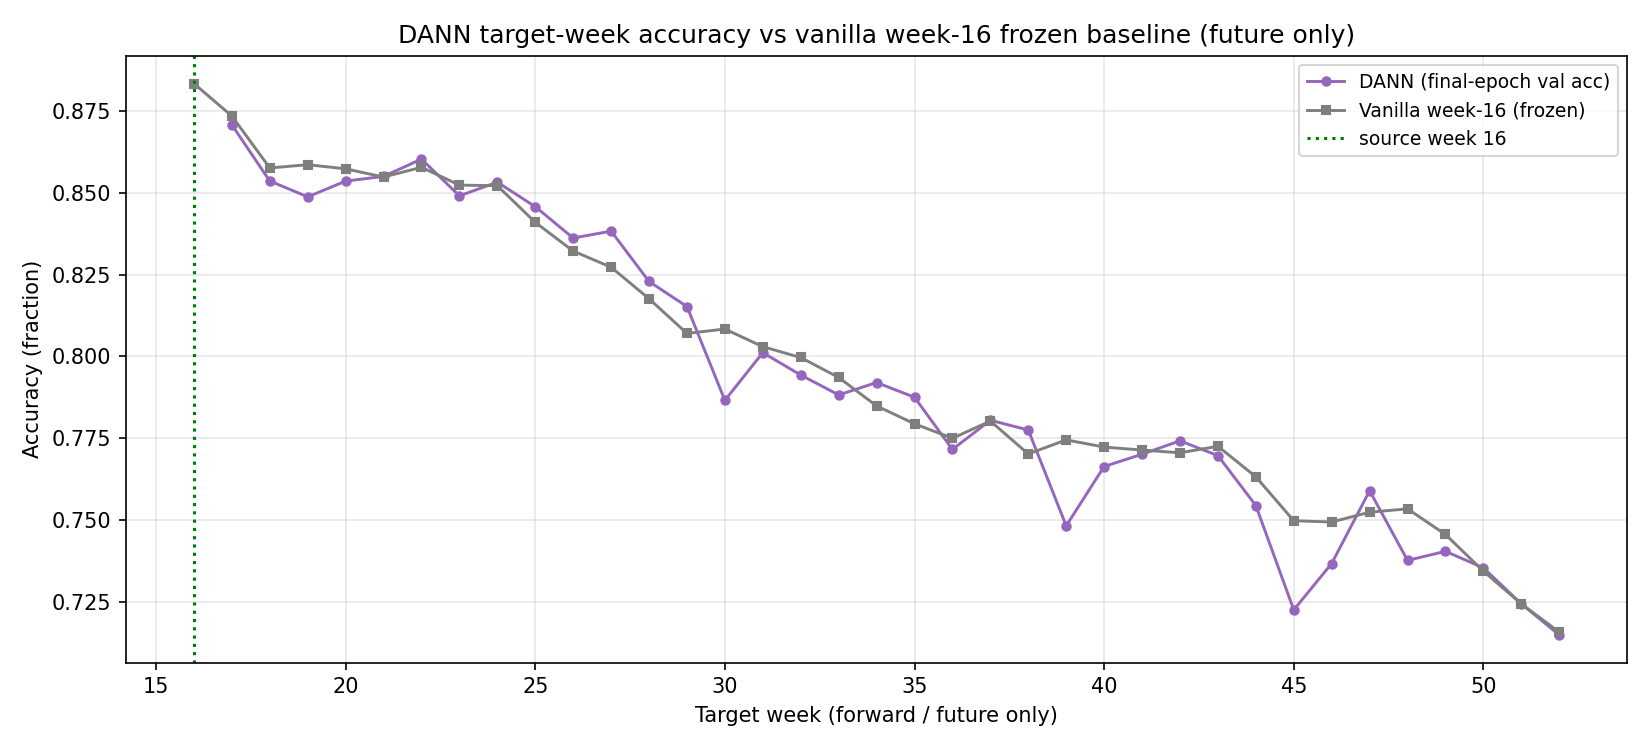
\includegraphics[width=\columnwidth]{figs/dann_vs_vanilla_acc_vs_week_future.png}}
\caption{DANN target-week accuracy vs the frozen Week-16 source, forward (future-only).
A dedicated per-target-week DANN model tracks the frozen baseline almost exactly and
dips \emph{below} it on several far weeks: adversarial alignment buys no forward
robustness, mirroring the $+0.006$ mean of Table~\ref{tab:nt_dann}. \TODO{caption later.}}
\label{fig:dann_curve}
\end{figure}
%  (anonymized for double-blind review) reproduces the effect more strongly.
%  The summary prose IS now in the body ("External validation" paragraph): bs64
%  AdaBN -0.030 / TENT -0.211 / CoTTA -0.173; bs256 AdaBN -0.014 / TENT -0.114 /
%  CoTTA -0.107 (5-seed std <=0.001); DANN +0.011 (neutral). Numbers from
%  results/analysis/closedworld_negtransfer_quarter.json. Advisor note: the
%  expanded per-method TABLE and the t-SNE stay disclosure-gated -> bring them in
%  ONLY if disclosure is permitted AND naming/describing it does not deanonymize
%  us. Keep CONSISTENT with the appendix t-SNE -> both appear or both stay out.

%==============================================================================
\section{Methodology: Weaponizing Estimator Failure}
\label{sec:method}

\subsection{Entropy as an Error Proxy}
The softmax output entropy of a classifier is a well-established per-sample error
proxy: incorrect predictions tend to land near the decision boundary and so carry
higher entropy than confident, correct ones \cite{wang2020tent}. Fig.~\ref{fig:entropy}
confirms this on our data, with the entropy of incorrect predictions clearly
shifted above that of correct ones. Entropy alone, however, cannot separate a
benign volume spike from a structural break: a viral surge of an inherently
high-uncertainty application raises mean entropy without any loss of accuracy.
Distinguishing the two requires a \emph{baseline} for how much entropy the current
class mix should produce --- which motivates the residual of
Sec.~\ref{sec:residual}. We flag one bridge caveat resolved there:
Fig.~\ref{fig:entropy} is a per-sample distribution, whereas the residual is built
from the \emph{aggregate} predicted marginal; Sec.~\ref{sec:residual} reconciles
the two.

\begin{figure}[htbp]
\centerline{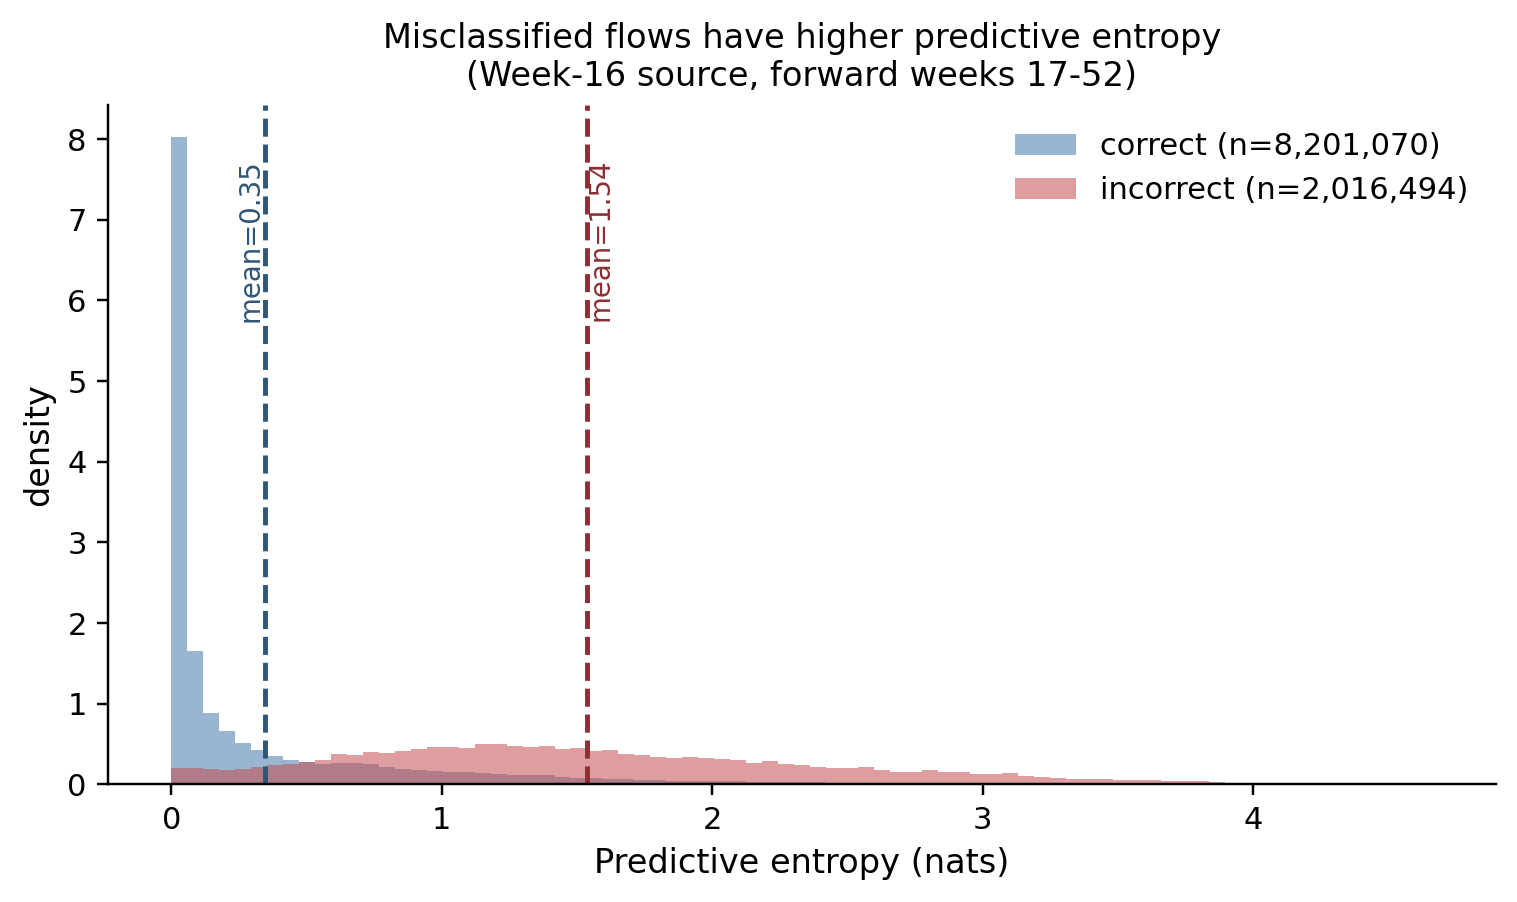
\includegraphics[width=\columnwidth]{figs/entropy_is_indicative.png}}
\caption{Predictive entropy is an error proxy: on Week-16-source frozen inference
(forward weeks 17--52), misclassified flows carry markedly higher entropy than
correct ones (mean $1.54$ vs $0.35$ nats).}
\label{fig:entropy}
\end{figure}

\subsection{BBSE: Robust to Label Shift, Shattered by Covariate Shift}
\label{sec:breakdown}
BBSE recovers the target label proportions from a frozen classifier's
predictions under the assumption that $P(X\mid Y)$ is invariant
\cite{lipton2018bbse}. That single assumption yields two opposite behaviors, and
the residual exploits the gap between them. In \textbf{Regime~1}
(Fig.~\ref{fig:regime1}, Week-16), where the shift is pure label shift and
$P(X\mid Y)$ stays intact, BBSE, RLLS, and EM-MLLS all hold a flat, low error
floor across injected severities $s\in[0,4]$ (60 draws per level, weeks 13--20),
while a static-prior baseline is roughly $11\times$ worse
\cite{lipton2018bbse,azizzadenesheli2019rlls}. This is the premise for the
$\Delta H_t\approx0$ arm of the residual: when the model has only seen a label
shift, the estimated proportions $\mathrm{w}_t$ are trustworthy. We note that
EM-MLLS is the \emph{most} accurate estimator in this regime, a point that becomes
important when we contrast estimation accuracy with detection robustness in
Sec.~\ref{sec:isolation}.\footnote{CESNET's dynamic per-service sampling flattens
label proportions, so the dataset-space shift understates the true network-space
shift; we therefore also re-project to approximate network proportions (the exact
ratios are unpublished). The same $\approx11\times$ gap and identical estimator
ordering hold in both spaces, so this sampling artifact does not affect the
covariate, per-class-$F_1$, or teleportation conclusions \cite{hynek2024cesnet}.}
In \textbf{Regime~2} (Fig.~\ref{fig:regime2}, Week-1), at the documented Week-10
covariate shift, the $L_1$ error of BBSE, RLLS, and SLD-EM \emph{spikes together}
\cite{saerens2002sld,garg2020mlls,ziegler2023bayesian} --- the premise for the
$\Delta H_t\gg0$ anomaly arm. We do not use these estimators to evaluate
corrective accuracy; we weaponize their shared, simultaneous breakdown as the
detector itself.

\begin{figure}[htbp]
\centerline{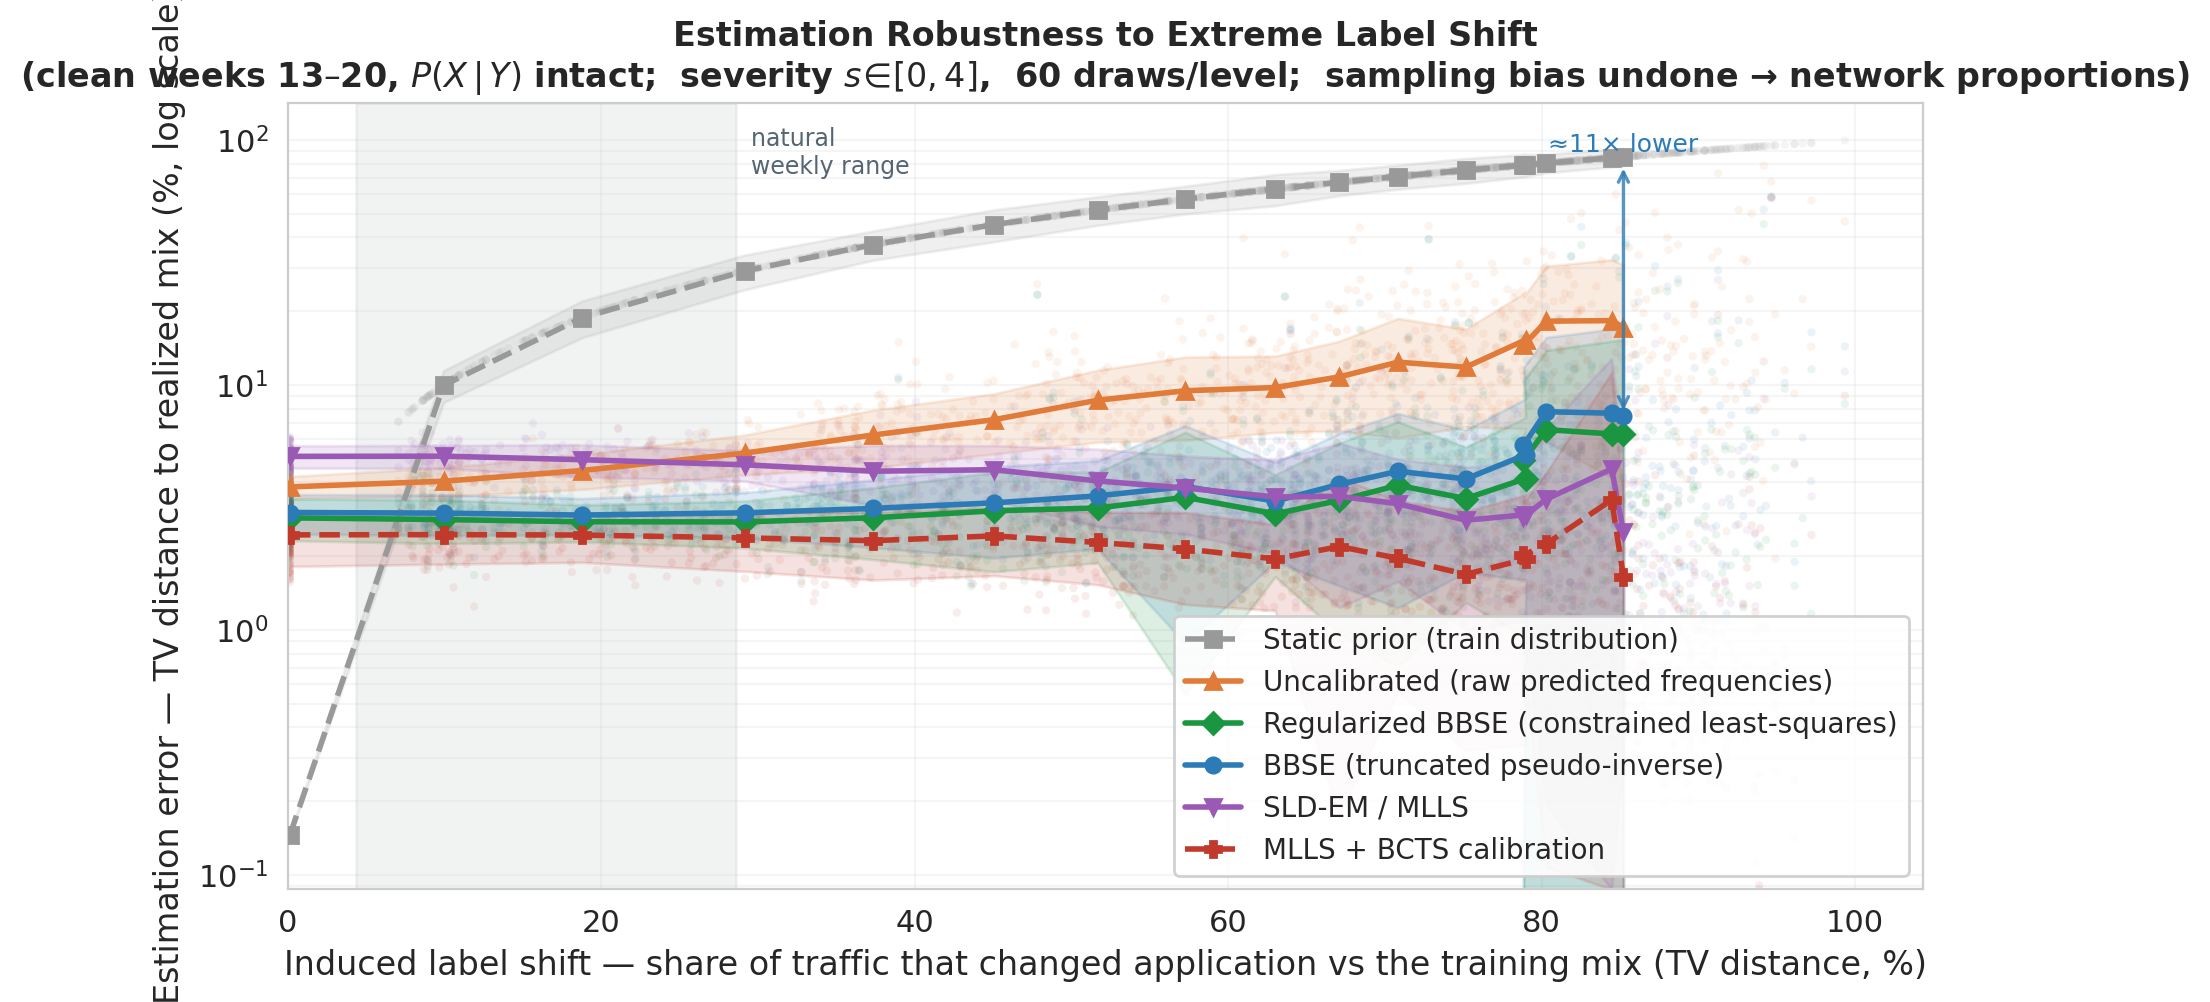
\includegraphics[width=\columnwidth]{figs/fig_estimation_robustness_severity_ref16_debiased.png}}
\caption{Regime 1 (Week-16): estimation robustness to extreme \emph{label} shift
with $P(X\mid Y)$ intact; $x$=TV-distance \% (network-reprojected). Estimators
flat; static prior tracks $y{=}x$ ($\approx$11x). Premise for $\Delta H_t\approx0$.
\TODO{caption later.}}
\label{fig:regime1}
\end{figure}

\begin{figure}[htbp]
\centerline{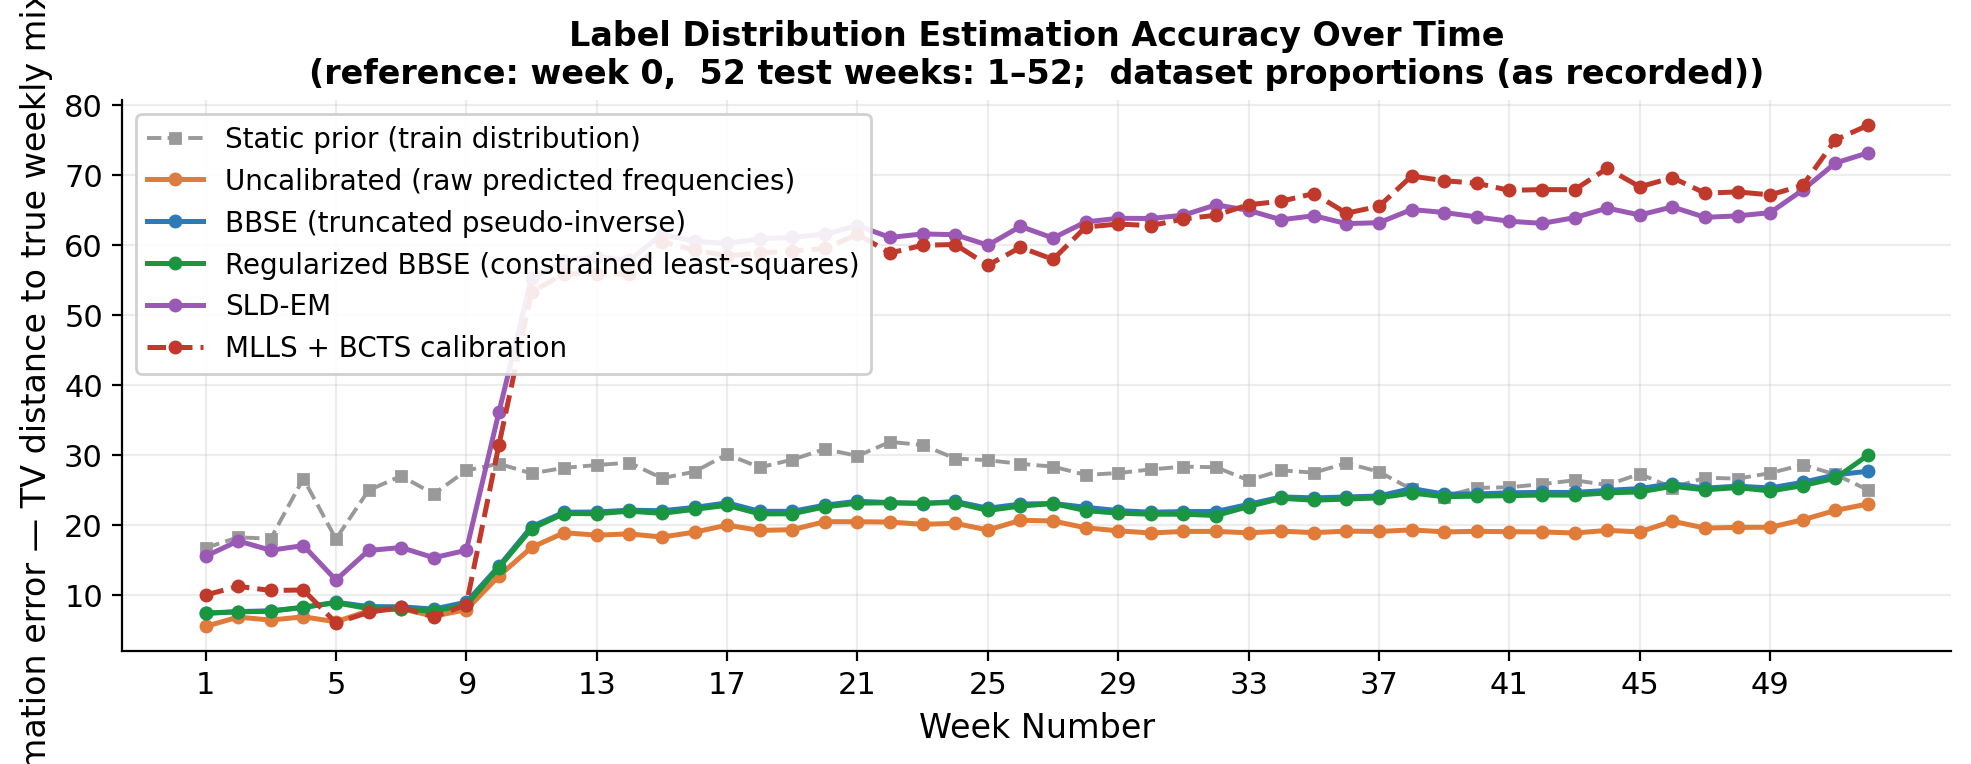
\includegraphics[width=\columnwidth]{figs/fig_estimation_accuracy (1).png}}
\caption{Regime 2 (Week-1, CORRECTLY): the documented Week-10 \emph{covariate}
shift spikes all estimators' $L_1$ error simultaneously. Premise for
$\Delta H_t\gg0$. \TODO{caption later.}}
\label{fig:regime2}
\end{figure}

\subsection{The BBSE-Corrected Entropy Residual}
\label{sec:residual}
We define the monitor's signal as the residual
\[
  \Delta H_t \;=\; H\!\big(P(\hat Y_t)\big) \;-\; H_{\mathrm{BBSE}}(\mathrm{w}_t).
\]
The first term is the Shannon entropy of the \emph{aggregate} predicted-label
marginal --- the mean softmax over the window, a class-balance quantity. The second
is the entropy of the BBSE-estimated true proportions $\mathrm{w}_t$. This is the
point at which the per-sample/aggregate caveat from Sec.~\ref{sec:method} is
reconciled: by Jensen's inequality $H(\mathbb{E}_x[p])\geq\mathbb{E}_x[H(p)]$, so the
entropy of the aggregate marginal is not the mean per-sample entropy of
Fig.~\ref{fig:entropy} but an upper envelope of it, and it is this envelope that
the residual interrogates.

The mechanism follows from the two regimes of Sec.~\ref{sec:breakdown}. Under a
benign \emph{label} shift, the predicted marginal moves but BBSE explains the move,
so $H(P(\hat Y_t))$ and $H_{\mathrm{BBSE}}(\mathrm{w}_t)$ rise together and the
residual stays near zero (the Regime-1 arm, Fig.~\ref{fig:regime1}). Under a
\emph{covariate} shift, the model's predictions for the broken class go flat and
dispersed, the aggregate marginal flattens artificially, and $H(P(\hat Y_t))$
inflates beyond what the (now-corrupted) $\mathrm{w}_t$ can account for, so the
residual spikes (the Regime-2 arm, Fig.~\ref{fig:regime2}). The residual is thus a
two-sided instrument: deliberately blind to label shift, and sharply responsive
to the covariate breaks that signal genuine degradation.

%==============================================================================
\section{Experimental Evaluation of the Monitor}
\label{sec:eval}
%  CONSOLIDATED: mirror -> primary viral-spike -> isolation -> estimator sweep.

\subsection{The Mirror Effect: Tracking Without Labels}
\label{sec:mirror}
Our first question is whether the residual tracks the model's hidden accuracy
without any labels. On clean forward data from the Week-16 source (weeks 17--52,
Fig.~\ref{fig:mirror}), it does, and so does its uncorrected counterpart: the
correlation between the entropy gap and the true Macro-$F_1$ is $\rho=-0.983$ for
the uncorrected gap, $-0.988$ for the BBSE-corrected residual, $-0.992$ for RLLS,
and $-0.991$ for an oracle that is handed the true proportions. We state plainly
that BBSE correction does \emph{not} improve clean tracking --- nor is it meant to;
its purpose is robustness, established in the next subsection. Two further points
come for free from this figure. First, the oracle line sits essentially on top of
BBSE and RLLS, so a better estimator could not track meaningfully better; clean
tracking is already near its ceiling. Second, SLD-EM \emph{inverts} on this data,
reaching $\rho=+0.030$ --- a striking failure that doubles as the visual evidence
for the estimation/detection dissociation we argue in Sec.~\ref{sec:sweep}. The
Week-1 mirror, which tracks the model \emph{through} the documented Week-10 event
at $\rho=-0.997$ (uncorrected) and $-0.994$ (BBSE), is deferred to Appendix
Fig.~\ref{fig:app_mirror_w1}. The per-class degradation grid
(Fig.~\ref{fig:grid}) makes the same point class by class: the top classes hold
and then drop in isolated step functions, and the BBSE proportions decouple from
the true volumes once a class breaks --- foreshadowing why the residual fires.

\begin{figure}[htbp]
\centerline{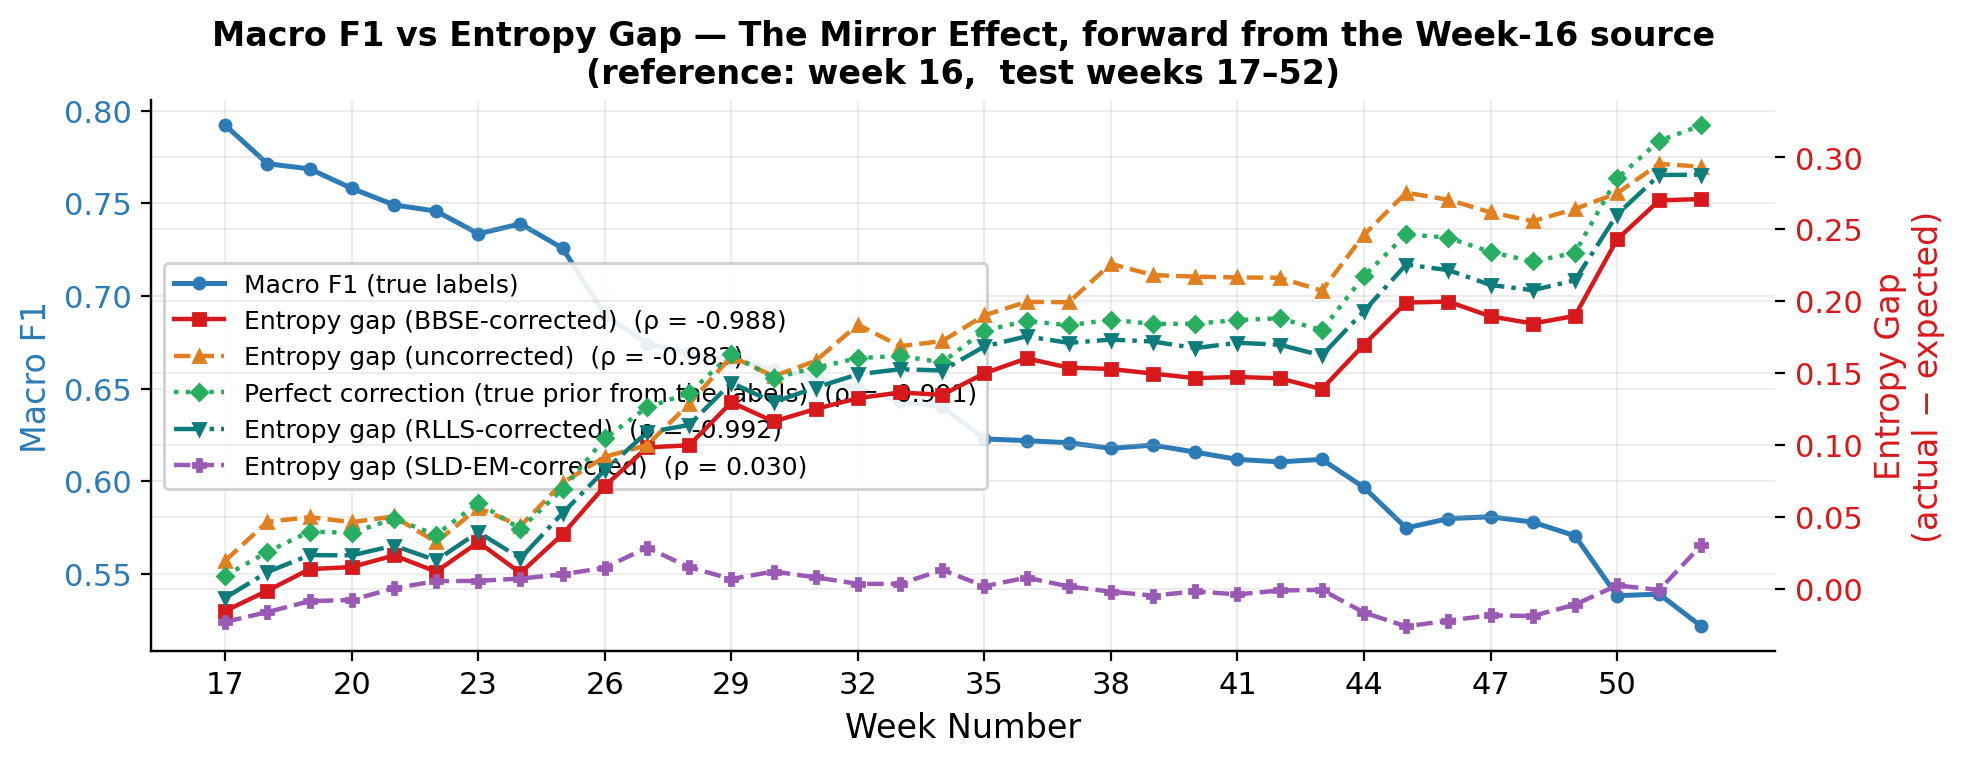
\includegraphics[width=\columnwidth]{figs/fig_mirror_effect_fwd.png}}
\caption{The Mirror Effect, forward from the Week-16 source (weeks 17--52,
PRIMARY). Uncorrected $\rho=-0.983$, BBSE $-0.988$, RLLS $-0.992$, oracle
$-0.991$; SLD-EM \emph{inverts} ($\rho=+0.030$) --- the visual evidence for the
estimation/detection dissociation (Sec.~\ref{sec:sweep}). \TODO{caption later.}}
\label{fig:mirror}
\end{figure}

\begin{figure}[htbp]
\centerline{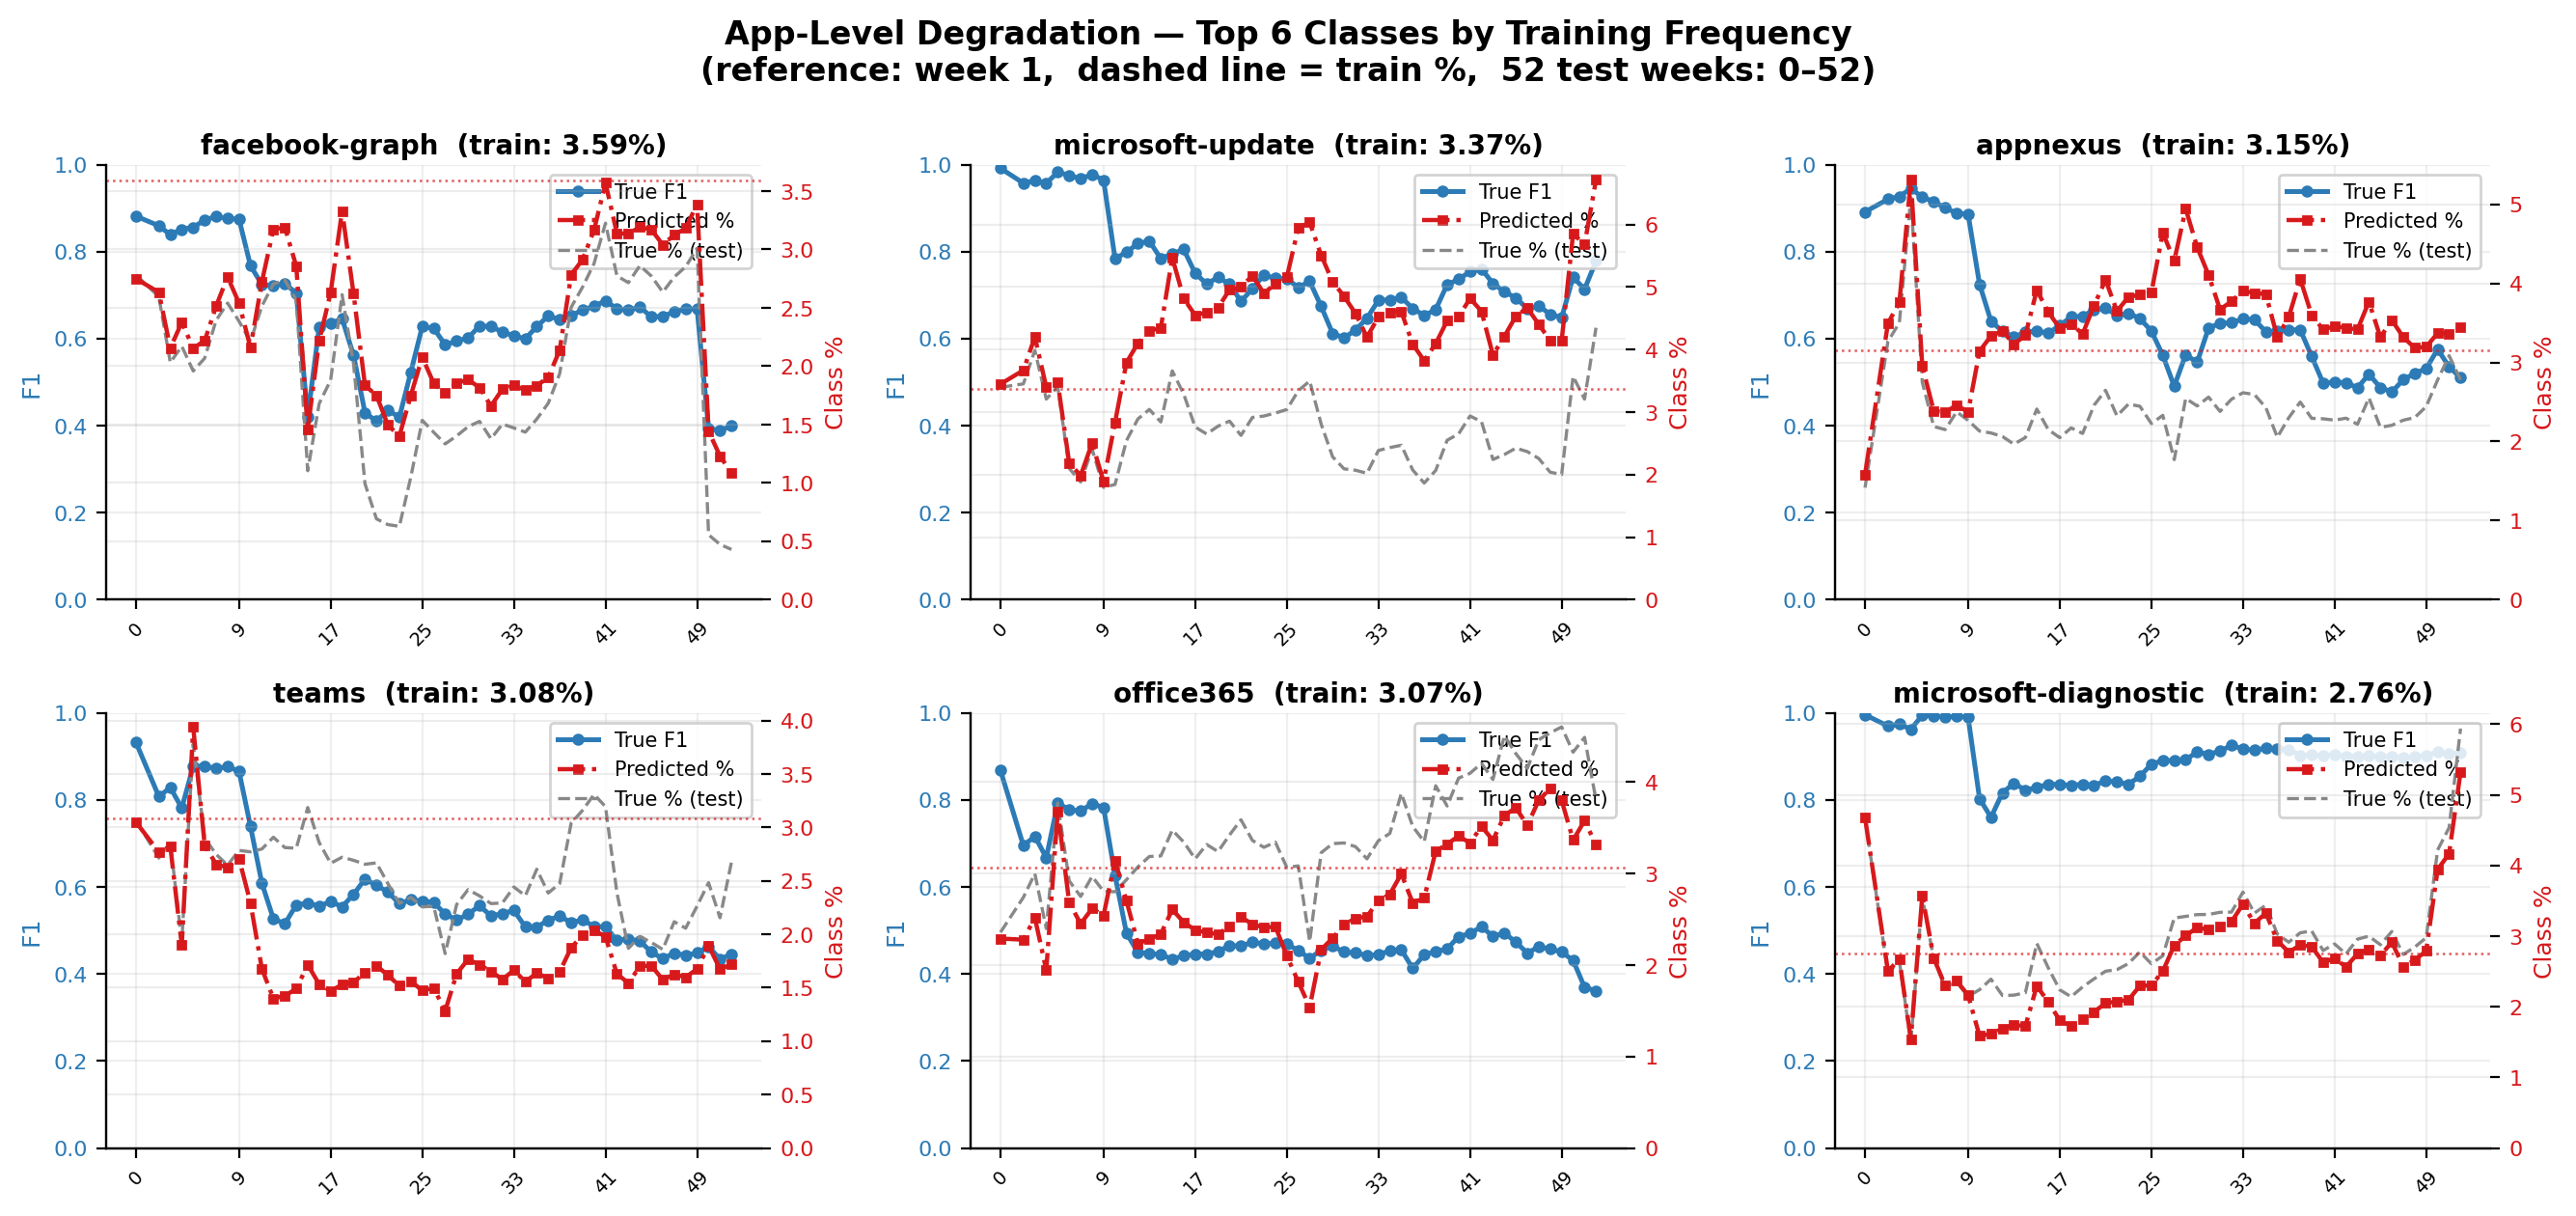
\includegraphics[width=\columnwidth]{figs/fig_app_degradation_grid.png}}
\caption{Per-class degradation grid: true F1 crashes independently; BBSE
proportions decouple from true volume. \TODO{Week-16 regeneration candidate.}}
\label{fig:grid}
\end{figure}

\subsection{Robustness Under Benign Volume Volatility (Primary Result)}
\label{sec:robustness}
Correlation, as the previous subsection showed, is the wrong axis on which to
compare detectors: on clean data every detector achieves AUROC$\approx1.000$
(Fig.~\ref{fig:auroc}(a)). The discriminating axis is \emph{robustness} --- whether
a monitor alarms on genuine degradation while staying silent under benign volume
volatility. We frame this as binary anomaly detection. The monitor sees only the
frozen model's unlabelled predictions, and a week is labeled anomalous iff its
true Macro-$F_1$ falls below 0.60. The ground truth is cause-agnostic: it includes
the Week-10 sensor event, which an operator would legitimately want flagged. The
benign stressor is a single-application viral spike, in which one application is
upsampled to a fraction $f\in[0.30,0.85]$ of an 8k-flow window while its
class-conditionals are left untouched. Because the spike never changes any class's
true degradation status --- the spiked application's own $F_1$ stays near 0.83 (and
0.766 on the Week-16 stream) --- every alarm it provokes on a healthy week is, by
construction, a false alarm.

\paragraph{Threat model.} Viral traffic is inherently asymmetric: one application
surges on what is typically a high-uncertainty class, so the asymmetric single-app
spike is the realistic stressor. The adversarial null is a \emph{symmetric}
LogUniform shift that perturbs all proportions at once. Under the symmetric null
(Fig.~\ref{fig:symmetric}) all detectors stay strongly correlated with hidden
$F_1$ but degrade gracefully with severity --- uncorrected
$-0.983\!\to\!-0.938$ ($10\times$) $\!\to\!-0.845$ ($100\times$), BBSE
$-0.988\!\to\!-0.951\!\to\!-0.892$, RLLS tracking BBSE, and SLD-EM worst
($-0.499/-0.659$). BBSE and RLLS are thus more robust even symmetrically, but the
sharp \emph{false-alarm} divergence that motivates correction appears only under
the asymmetric spike.

\paragraph{Results.} On the Week-1 stream, which carries the degraded-week
positives needed for the healthy-vs-degraded split, the BBSE-corrected residual
reaches AUROC 0.987 at a false-alarm rate of 4.6\% under 95\% matched detection,
against 0.959 / 25.0\% for the uncorrected entropy gap and 0.677 / 64.8\% for the
MFWDD-style global detector (Fig.~\ref{fig:auroc}(b), Table~\ref{tab:auroc}) --- a
$5.4\times$ and $14\times$ reduction in false alarms; at 90\% detection the gap is
2.8\% vs 12.0\% vs 59.3\%. The mechanism is score-level: a viral spike inflates the
uncorrected entropy gap into the degradation band, whereas BBSE recognizes the
over-represented application, raises the expected entropy accordingly, and pulls
the residual back below threshold. MFWDD is worst precisely because a global
feature distance cannot tell a benign surge from a structural break.

\paragraph{Week-16 replication.} To confirm the advantage is not an artifact of
the Week-10 sensor event, we repeat the experiment entirely within the clean
Week-16 forward regime (5 seeds, Table~\ref{tab:auroc_w16}). Here the clean regime
is trivial for every detector (AUROC$\approx1.000$, FAR$_{95}\approx0$), and under
the viral spike the corrected estimators again separate from the rest: BBSE 0.834,
RLLS 0.849, MLLS+BCTS 0.827, all well above uncorrected 0.708 and MFWDD-style
0.650 (SLD-EM 0.759). At 95\% matched detection the BBSE residual holds a 0.675
false-alarm rate against uncorrected's 0.837. The absolute AUROCs are lower than
on Week-1 because the Week-16 viral task is harder --- there is no large sensor
break inflating the positives --- but the ordering is unchanged, so the
correction's benefit is intrinsic to the asymmetric-spike stressor, not a
by-product of the sensor event.

\begin{figure}[htbp]
\centerline{
\includegraphics[width=\columnwidth]{figs/fig_auroc_anomaly.png}}
\caption{Binary anomaly detection (Week-1; dotted=95\% matched detection).
(a) clean: all perfect. (b) viral spikes: ours 0.987 dominates uncorrected
0.959 and MFWDD-style 0.677. \TODO{caption later.}}
\label{fig:auroc}
\end{figure}

\begin{table}[t]
\caption{Binary anomaly detection under a viral single-app spike: AUROC and
FAR@95\% matched detection. Clean rows omitted (all AUROC 1.000, FAR 0\%).
Confusion-matrix estimators suppress false alarms; EM/MLLS gives little benefit
(SLD-EM ties uncorrected); MFWDD-style fails.}
\label{tab:auroc}
\centering
\begin{tabular}{llcc}
\toprule
Regime & Detector & AUROC & FAR@95 \\
\midrule
Viral & \textbf{BBSE-corrected (ours)} & \textbf{0.987} & \textbf{4.6\%} \\
Viral & Soft-confusion BBSE      & 0.988 & 6.5\% \\
Viral & RLLS                     & 0.982 & 7.4\% \\
Viral & Uncorrected entropy gap  & 0.959 & 25.0\% \\
Viral & MLLS+BCTS                & 0.953 & 17.6\% \\
Viral & SLD-EM / MLLS            & 0.946 & 25.0\% \\
Viral & MFWDD-style global       & 0.677 & 64.8\% \\
\bottomrule
\end{tabular}
\end{table}

\begin{table}[t]
\caption{Week-16 forward replication of the viral anomaly experiment (5 seeds;
weeks 17--52, $F_1<0.6$). Clean regime omitted (all AUROC $\approx$1.000,
FAR$_{95}\approx0$). The corrected estimators again lead; absolute AUROC is lower
than on Week-1 (Table~\ref{tab:auroc}) because the clean-regime task carries no
sensor-break positives, but the ordering is unchanged.}
\label{tab:auroc_w16}
\centering\small
\begin{tabular}{lcc}
\toprule
Detector (viral) & AUROC & FAR@95 \\
\midrule
RLLS                          & 0.849 & 0.49 \\
Soft-confusion BBSE           & 0.836 & 0.73 \\
\textbf{BBSE-corrected (ours)}& \textbf{0.834} & \textbf{0.68} \\
MLLS+BCTS                     & 0.827 & 0.68 \\
SLD-EM / MLLS                 & 0.759 & 0.88 \\
Uncorrected entropy gap       & 0.708 & 0.84 \\
MFWDD-style global            & 0.650 & 0.73 \\
\bottomrule
\end{tabular}
\end{table}

\paragraph{Statistical rigor and threshold sensitivity.} To verify that the
Week-16 ordering is not a chance artifact of the seeds or of the anomaly cutoff,
we run a separate forward-only experiment with a block bootstrap (2000 resamples
over week clusters with the five seeds nested, since the anomaly label is keyed on
the week; this is a distinct experimental stream from the injection study above and
its absolute AUROCs are not directly comparable to Table~\ref{tab:auroc_w16}). At
the headline $F_1<0.6$ cutoff (Table~\ref{tab:statrigor}), the BBSE residual reaches
AUROC 0.690, ahead of uncorrected (0.627) and MFWDD-style (0.577). With only 36
week-level clusters the 95\% intervals are wide and the BBSE and uncorrected bands
overlap (0.690\,[0.633,\,0.745] vs 0.627\,[0.585,\,0.669]), so we do not claim
interval-level separation; the support for BBSE's advantage is instead the
consistent point-estimate ordering and its stability across the anomaly cutoff.
Sweeping the Macro-$F_1$ threshold over $\{0.55,0.60,0.65\}$ yields BBSE AUROC
$0.713/0.690/0.748$, beating uncorrected ($0.614/0.627/0.654$) and MFWDD-style at
every cutoff --- the advantage is not threshold-cherry-picked.

\begin{table}[t]
\caption{Statistical rigor on the Week-16 forward viral stream (block bootstrap,
2000 resamples over week clusters with seeds nested, 95\% percentile CI; headline
$F_1<0.6$). With 36 week-level clusters the intervals are wide and overlap; the
point-estimate ordering and the threshold sweep, not the CIs, carry the result.
Frozen-source vanilla inference at 10\% sample --- do not cross-compare these
absolute AUROCs to the injection study (Table~\ref{tab:auroc_w16}).}
\label{tab:statrigor}
\centering\small
\begin{tabular}{lc}
\toprule
Detector (viral, forward) & AUROC [95\% CI] \\
\midrule
\textbf{BBSE-corrected (ours)} & \textbf{0.690 [0.633,\,0.745]} \\
Uncorrected entropy gap        & 0.627 [0.585,\,0.669] \\
MFWDD-style global             & 0.577 [0.541,\,0.618] \\
\bottomrule
\end{tabular}
\end{table}

\paragraph{Per-class out-of-distribution baselines.} The open-set framing of
Sec.~\ref{sec:related_osr} invites a direct comparison with per-class
out-of-distribution (OOD) scores. We add two: a per-class energy score
$E=-\log\!\sum\exp(\text{logits})$ and the maximum-softmax-probability (MSP)
baseline, both computed per class on the Week-16 forward stream
(Fig.~\ref{fig:ood}). In the \emph{clean} regime these are strong --- naive
uncorrected entropy detects degraded classes at AUROC 0.958 and MSP at 0.928,
ahead of our residual (0.878), energy (0.861), and MFWDD-style (0.710).\footnote{Our
residual and naive entropy are scored over all $n{=}4380$ class-weeks; energy, MSP,
and MFWDD-style are restricted to the $n{=}3509$ class-weeks whose 10\% embedding
subsample exceeds the minimum region size, so their absolute AUROCs are over a
slightly different population (this also accounts for the MFWDD-style 0.710 here vs
0.723 in the isolation ablation, a distinct forward stream).} The
picture inverts under a severity-1000 benign label shift: our residual degrades
\emph{least} (AUROC $0.893\!\to\!0.768$), while naive ($0.968\!\to\!0.671$), MSP
($0.934\!\to\!0.683$), and energy ($0.895\!\to\!0.664$) all drop sharply (to $\approx$0.66--0.68).
Per-class OOD scoring is thus competitive only in the clean regime and
false-alarms heavily under benign volume shift --- the same failure mode as
uncorrected entropy. This directly answers the ``why not compare to energy/OOD
methods'' question: the open-set framing is not merely interpretive, and our
correction is what makes the per-class signal robust where raw OOD scores are not.

\begin{figure}[htbp]
\centerline{
\includegraphics[width=\columnwidth]{figs/fig_ood_baseline_comparison.png}}
\caption{Per-class OOD baselines (Week-16 forward). Energy and MSP join naive
entropy and MFWDD-style detection. Left: clean-regime detection (naive/MSP
sharpest). Right: under severity-1000 benign label shift our residual degrades
least while naive, MSP, and energy collapse. \TODO{caption later.}}
\label{fig:ood}
\end{figure}

\begin{figure}[htbp]
% UPGRADED: two Week-16 forward symmetric-shift figures (was a single Week-1 panel).
\centerline{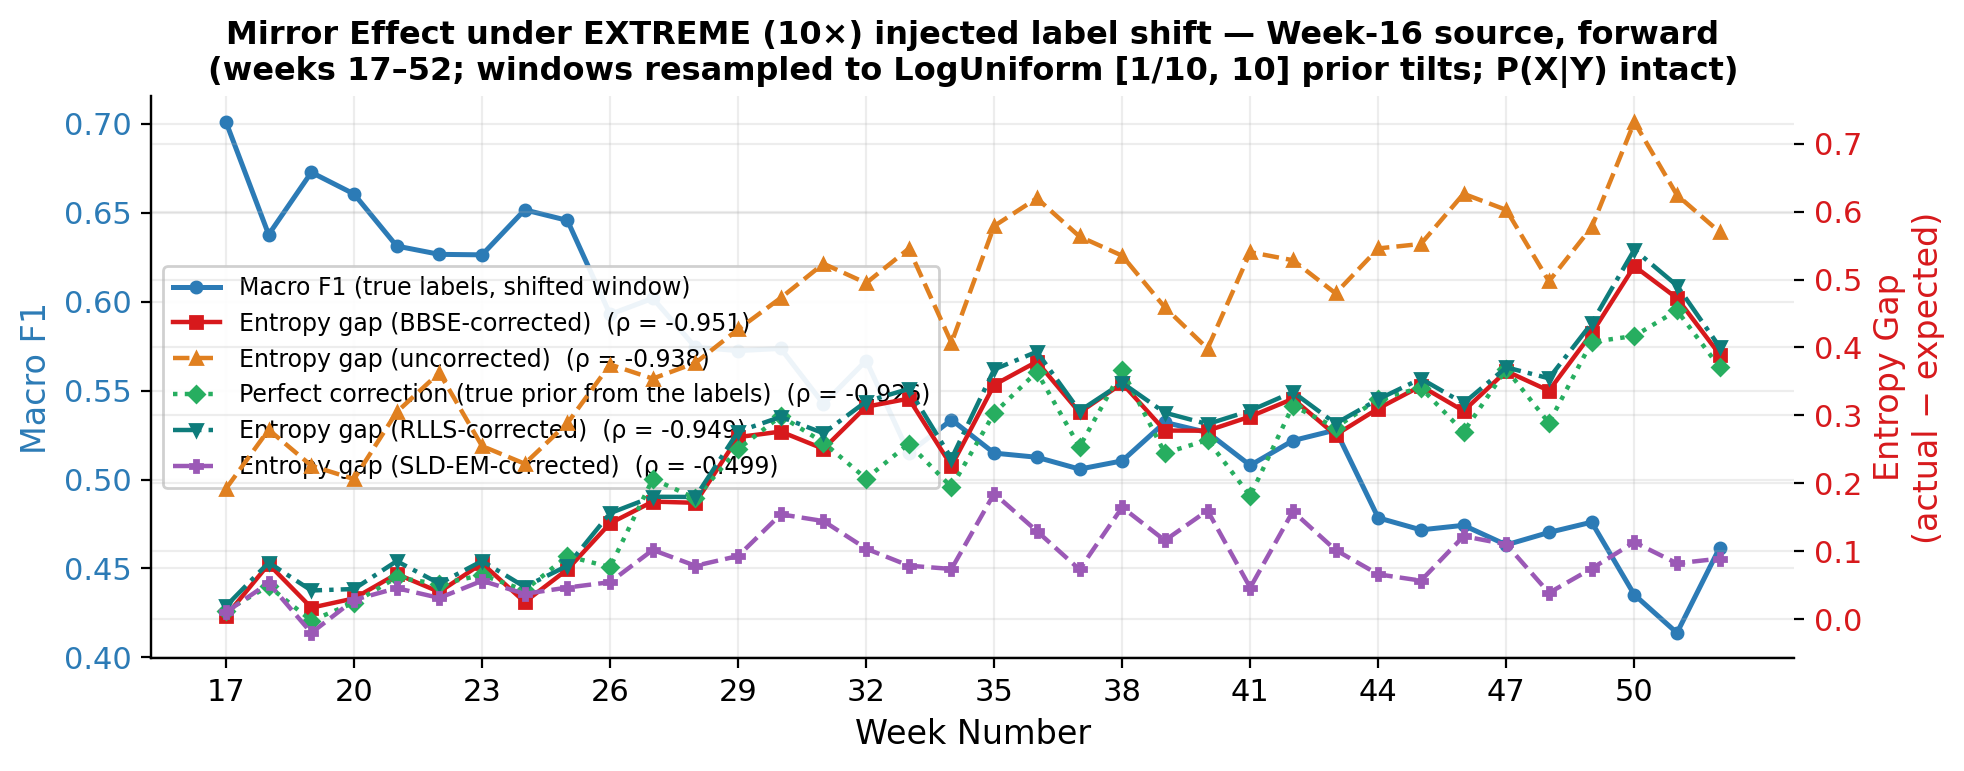
\includegraphics[width=\columnwidth]{figs/fig_mirror_extreme_fwd_10x.png}}
\centerline{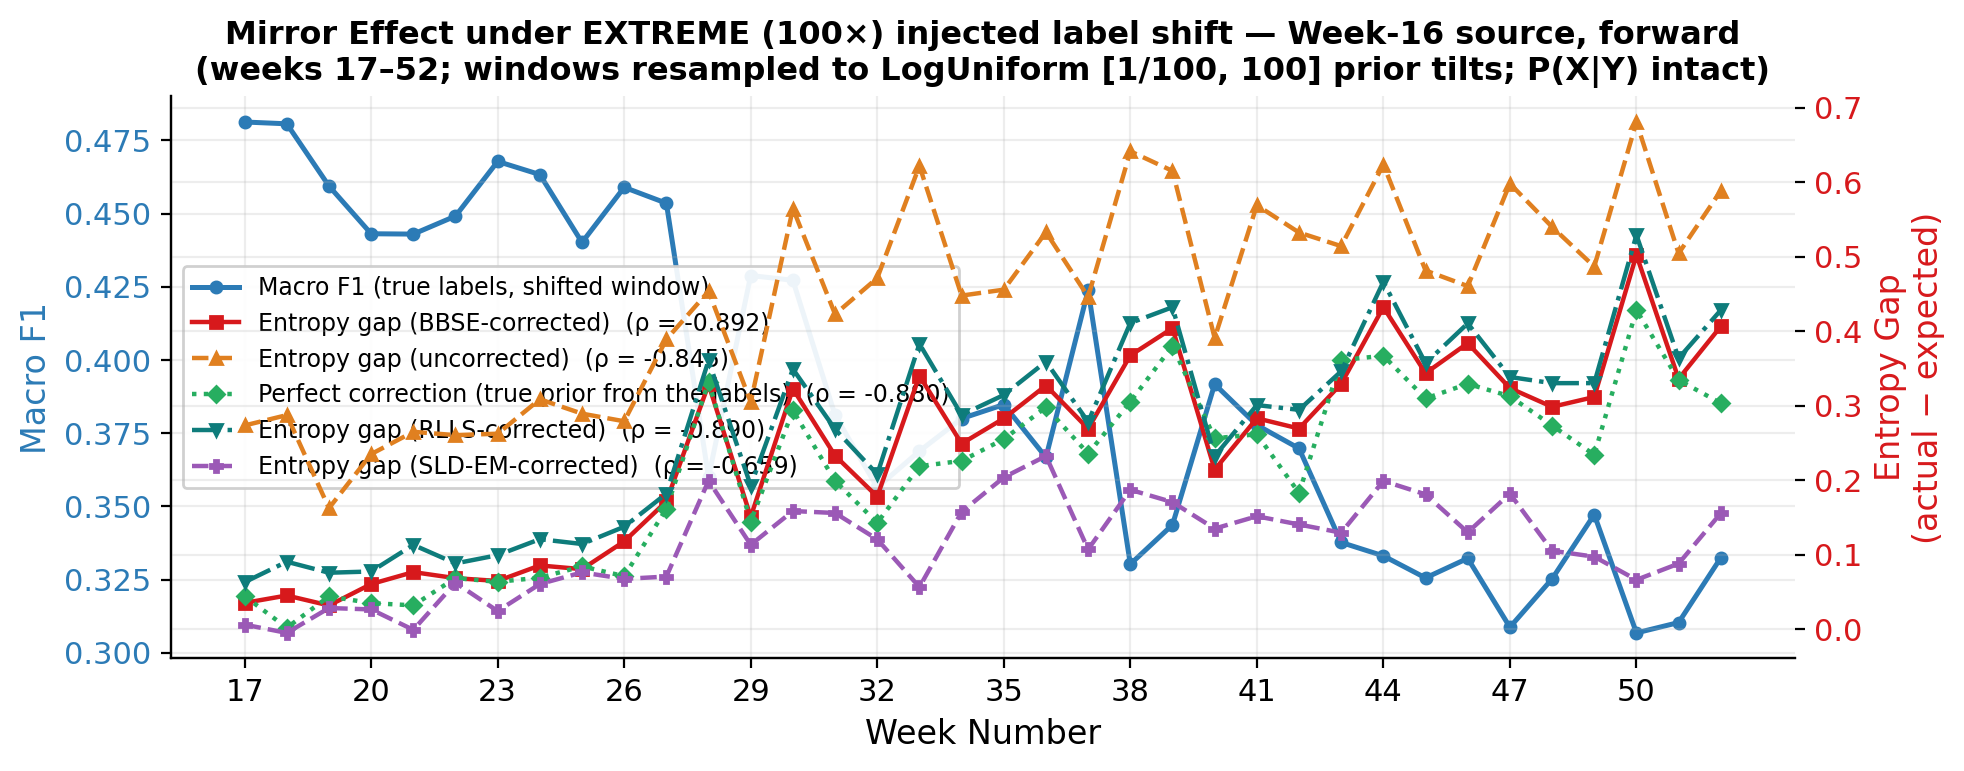
\includegraphics[width=\columnwidth]{figs/fig_mirror_extreme_fwd_100x.png}}
\caption{Symmetric robustness CONTROL (Week-16 forward), $10\times$ (top) and
$100\times$ (bottom) LogUniform label shift, $P(X\mid Y)$ intact. All gaps stay
correlated but degrade GRACEFULLY with severity; BBSE ($-0.951/-0.892$) and RLLS
degrade less than uncorrected ($-0.938/-0.845$); SLD-EM worst ($-0.499/-0.659$).
The asymmetric viral spike (Fig.~\ref{fig:auroc}) is the discriminating stressor.
\TODO{caption later; optionally move the $10\times$ panel to the appendix to save space.}}
\label{fig:symmetric}
\end{figure}

\subsection{Per-Class Isolation}
\label{sec:isolation}
The operational promise of the monitor is a per-class tripwire that fires on
genuinely degraded classes and not on healthy classes that merely changed volume.
We test this with an isolation ablation on the Week-16 stream
(Fig.~\ref{fig:isopanels}), where ``isolation'' means separating
genuinely-degraded from benignly-label-shifted classes without bleeding alarms
onto stable domains. On clean data, the uncorrected entropy gap is the sharpest
raw per-class detector (AUROC 0.958 vs ours 0.878 vs MFWDD-style 0.723), which
re-confirms that correction buys robustness rather than clean sharpness. Under
injected pure label shift, that sharpness becomes a liability: uncorrected floods,
bleeding alarms onto up to 0.48 of stable classes at $1000\times$ severity, while
our residual stays far lower at 0.18--0.27; MFWDD-style is near-inert here
(recall $\sim$0.01). The decisive view is separability under $1000\times$
contamination (Appendix Fig.~\ref{fig:app_panelC}): our residual degrades least
($0.88\!\to\!0.77$) and actually overtakes uncorrected, which collapses
($0.96\!\to\!0.67$), with MFWDD-style at $0.72\!\to\!0.57$. Finally, at matched
recall our detector disturbs consistently fewer healthy classes than either
baseline (15--38\% vs 35--46\% for naive and 44--70\% for MFWDD-style, up to
$\sim3\times$ fewer than MFWDD), with MFWDD-style worst once it is forced to a
useful recall. These isolated per-class flags are exactly the input the open-set
repair loop of Sec.~\ref{sec:operational} consumes
\cite{tao2020fscil,rebuffi2017icarl,kirkpatrick2017ewc,li2017lwf,shahraki2022active}.

\begin{figure}[htbp]
% Week-16 panels (author-added). Flat figs/ dir. Save the new A/B/D here.
\centerline{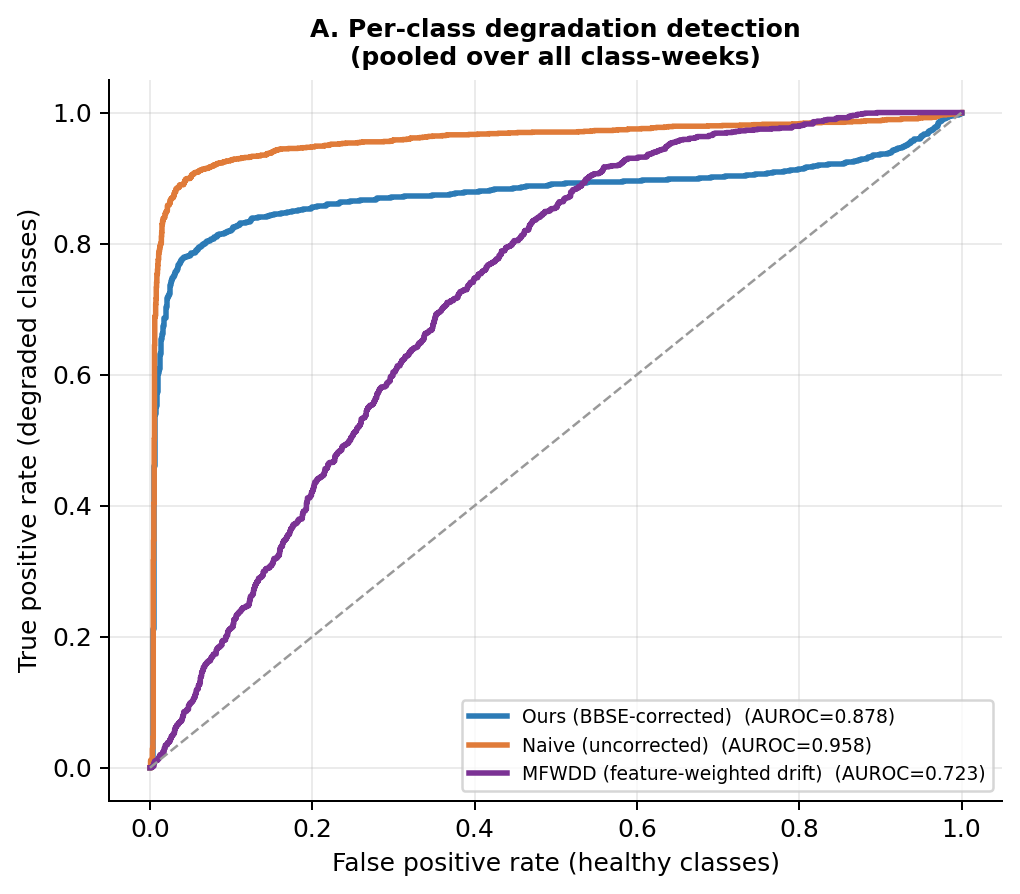
\includegraphics[width=\columnwidth]{figs/fig_isolation_A_roc_detection_fwd.png}}
\centerline{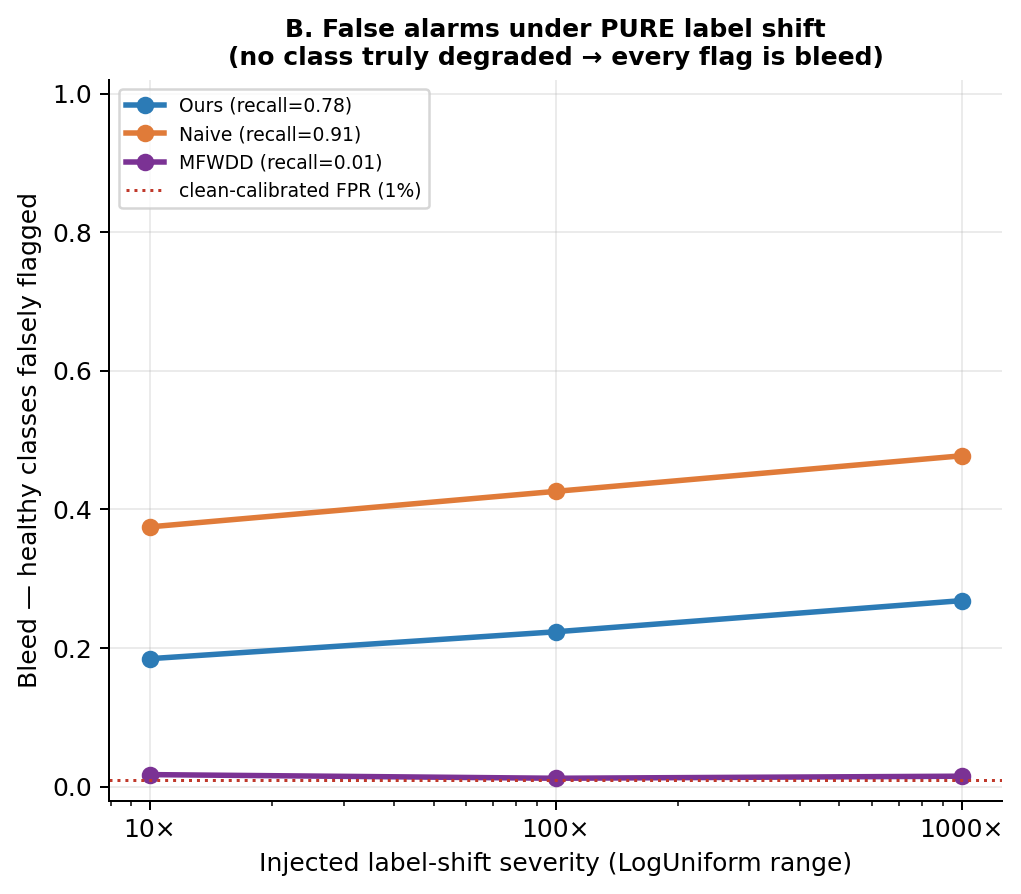
\includegraphics[width=0.49\columnwidth]{figs/fig_isolation_B_bleed_vs_severity_fwd.png}\hfill
            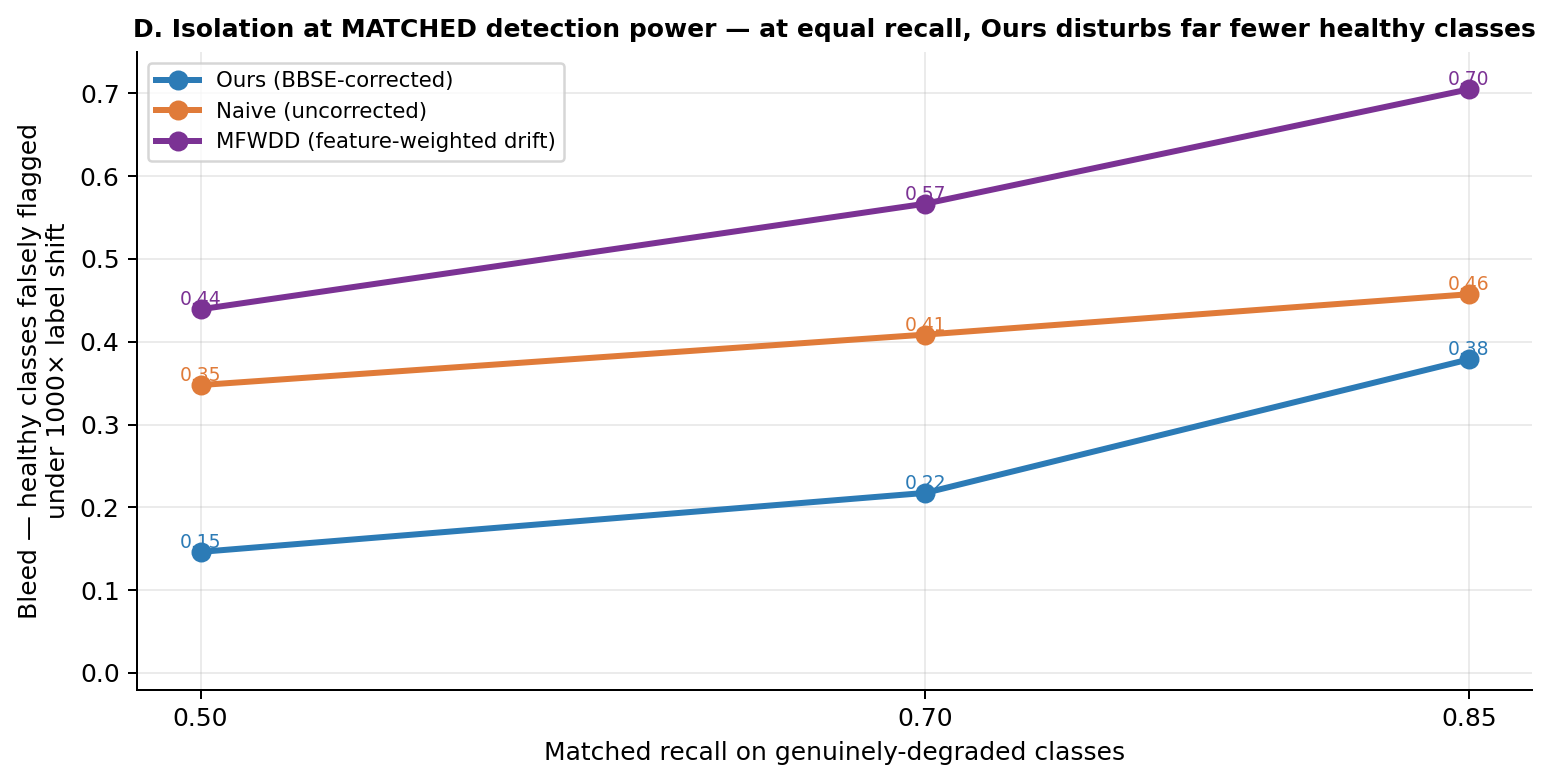
\includegraphics[width=0.49\columnwidth]{figs/fig_isolation_D_matched_recall_bleed_fwd.png}}
\caption{Isolation ablation (Week-16, forward-only stream, weeks 17--52). (a) clean: uncorrected
sharpest (0.96 vs 0.88). (b) label shift: uncorrected bleeds up to 0.48@1000x, ours
0.18--0.27. (d) matched recall: ours disturbs consistently fewer healthy classes
(15--38\% vs naive 35--46\% / MFWDD 44--70\%).}
\label{fig:isopanels}
\end{figure}

\subsection{Natural Volume Surges: An Honest Stress Test}
\label{sec:natural}
The synthetic stressors above are deliberately extreme. To gauge the monitor in
the wild, we also scan the Week-16 forward stream for \emph{real}, single-app
benign volume surges and compare them against genuinely degrading classes that
happen to surge at similar magnitudes (Fig.~\ref{fig:natural}). Four real benign
surges --- aukro-backend ($\times4.6$, recall 0.91), cesnet-kalendar ($\times4.2$,
0.92), owncloud ($\times4.1$, 0.83), and chmi ($\times3.3$, 0.93) --- are contrasted
with degrading classes of comparable surge (dopravni-info $>\!\times5$, recall
$\approx0.001$; riot-games $>\!\times5$, recall $\approx0.18$). The encouraging
finding is that the per-class corrected residual tracks \emph{recall} (i.e.\
degradation), not volume: the largest benign surge (aukro, $\times4.6$) produces a
residual of only $+0.38$ and chmi ($\times3.3$) only $+0.02$, while a degrading
riot-games surge produces $+1.29$.

We report the limitations honestly. At a strict 1\%-per-class false-alarm
threshold ($+0.350$), two of the four benign surges edge above it --- owncloud
($+0.61$) and aukro-backend ($+0.38$) --- a real, disclosed false alarm. These
benign surges sit in the same $\sim$99th residual percentile band as the flagged
riot-games degradations, so a single residual-magnitude threshold does \emph{not}
cleanly separate them. What separates them operationally is recall persistence:
the benign surges keep recall $\geq0.83$, whereas the degradations sit at
$\approx0.18$ or below. Separately, the worst degradations (dopravni-info at
recall $\approx0.001$) fully \emph{evacuate} their predicted region, leaving the
region-based residual undefined; these are caught by recall, a limitation of any
predicted-region detector rather than of BBSE specifically. Finally, on these
modest natural surges the corrected residual shows \emph{no} advantage over the
uncorrected one (it flags two benign surges to the uncorrected detector's one):
the large BBSE advantage materializes only under the extreme synthetic asymmetric
spikes (Sec.~\ref{sec:robustness}) and high-severity synthetic label shift
(Sec.~\ref{sec:isolation}), and we do not claim a clean natural win.

\begin{figure}[htbp]
\centerline{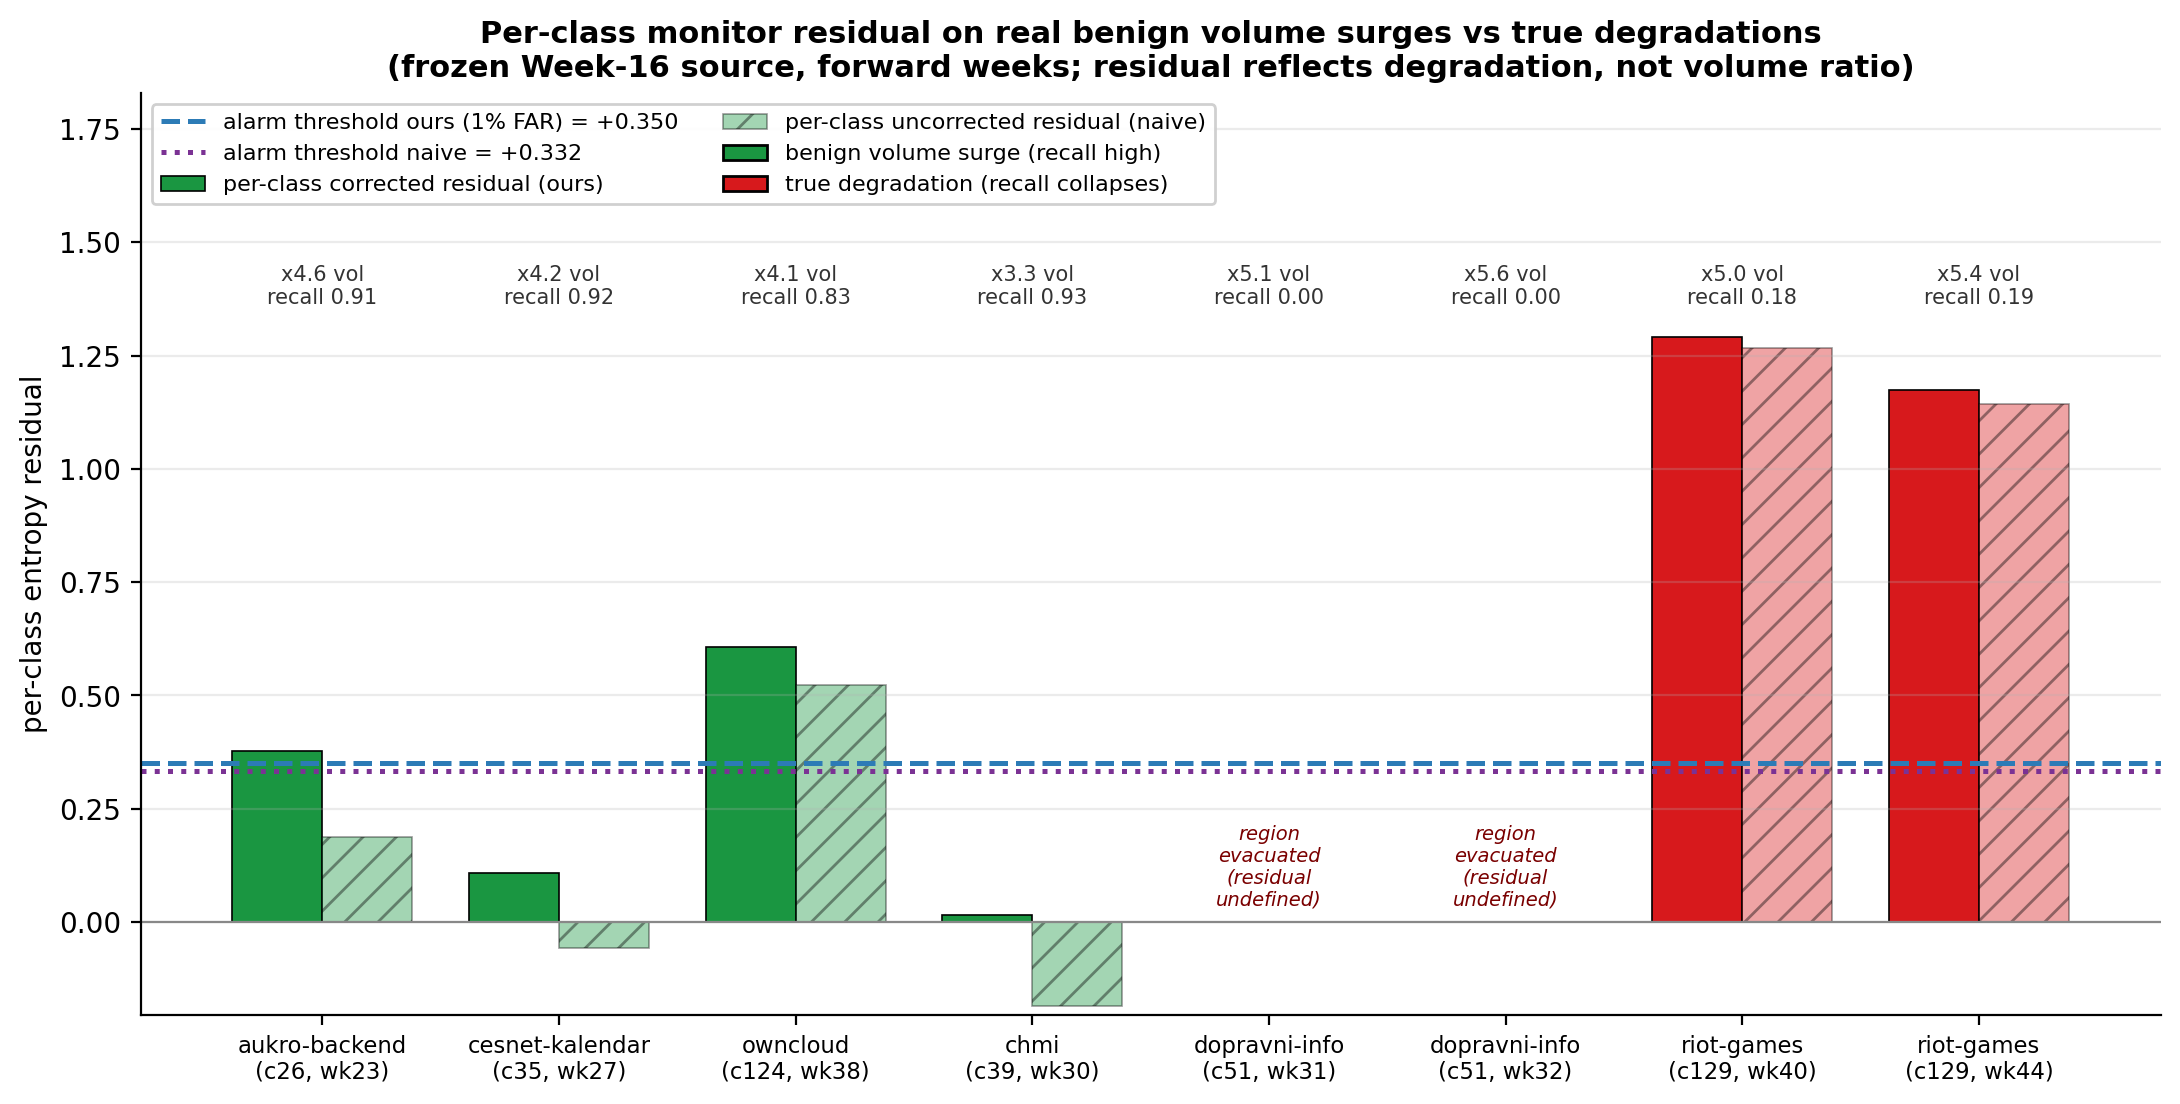
\includegraphics[width=\columnwidth]{figs/fig_natural_perclass_residual.png}}
\caption{Natural per-class volume surges (Week-16 forward): real benign single-app
surges vs degrading classes of similar magnitude. The corrected residual tracks
recall/degradation, not volume; two of four benign surges nonetheless edge above
the strict 1\%-FAR threshold, separated from genuine degradation only by recall
persistence.}
\label{fig:natural}
\end{figure}

\subsection{Estimator-Variant Sweep and the Estimation/Detection Dissociation}
\label{sec:sweep}
Two questions remain: does the isolation result depend on the choice of
estimator, and what is the uncorrected detector's clean-data sharpness actually
worth? We answer both by sweeping the injected label-shift severity $s$ on the
Week-16 stream (Fig.~\ref{fig:sweep}). At the mildest injected severity $s{=}1$ the
uncorrected detector indeed leads (0.921 vs 0.897 for BBSE), but its AUROC decays steeply, is overtaken by
BBSE between $s{=}3$ and $s{=}5$, and collapses to $\approx0.70$ at $s{=}1000$; BBSE,
soft-BBSE, and RLLS all hold near 0.80, while EM/MLLS decays faster. The
uncorrected detector, in short, looks best only when there is nothing to be
robust to.

This exposes a clean \emph{estimation/detection dissociation}. EM/MLLS is the
\emph{most accurate} label-shift estimator in the robustness benchmark
(Fig.~\ref{fig:regime1}), yet it is the \emph{least robust} detector here; SLD-EM
even inverts to $\rho=+0.030$ on the Week-16 mirror (Fig.~\ref{fig:mirror}) and
ties the uncorrected false-alarm rate under a viral spike
(Table~\ref{tab:auroc}). Estimation accuracy and detection robustness are
therefore not the same objective in our experiments. Our verdict is to
keep plain BBSE: soft-confusion BBSE is a near-equivalent swap, RLLS ties, and
EM/MLLS is disqualified for this use. Both this sweep and the isolation ablation
now run on Week-16, keeping the clean-regime analyses internally consistent.

\begin{figure}[htbp]
\centerline{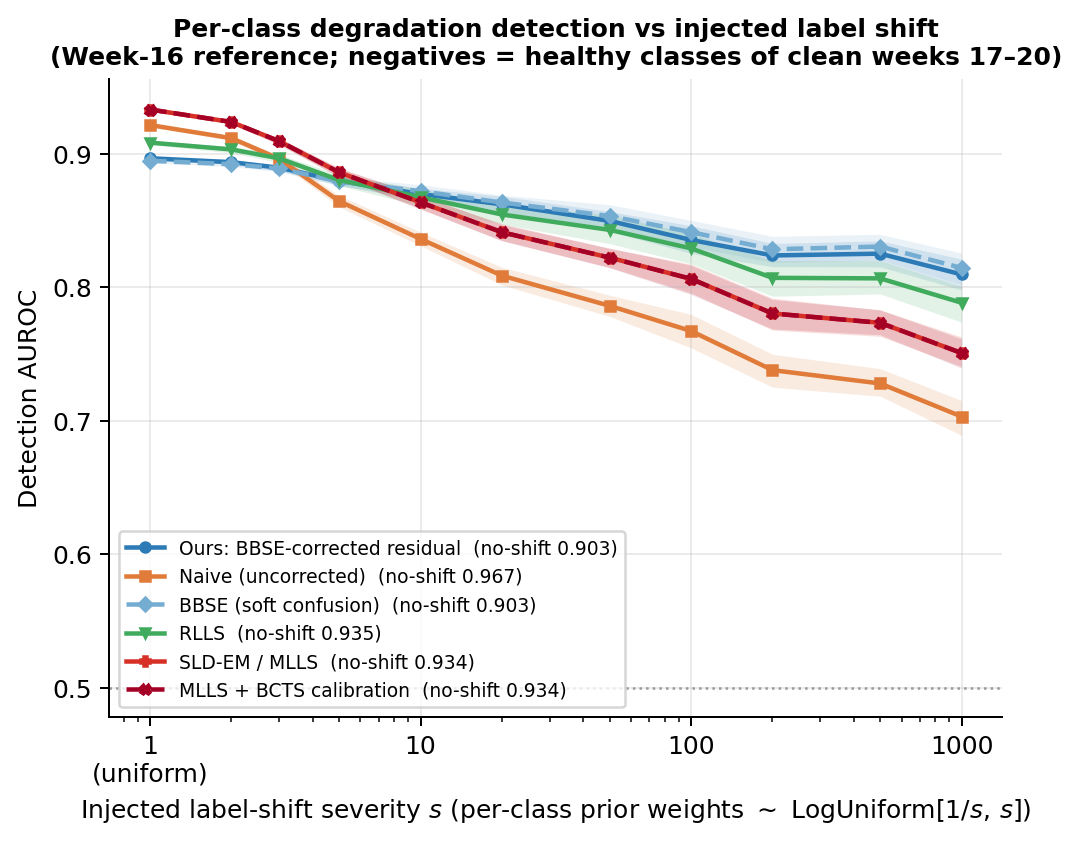
\includegraphics[width=\columnwidth]{figs/fig_isolation_auroc_vs_labelshift_estimators_fwd.png}}
\caption{The uncorrected detector's clean-data lead is fragile. Detection AUROC
vs label-shift severity $s$ (Week-16; weights $\sim$LogUniform$[1/s,s]$).
Uncorrected leads at $s{=}1$ (0.921 vs 0.897) but is overtaken between $s{=}3$ and
$s{=}5$ and reaches $\approx0.70$ at $s{=}1000$; corrected estimators stay near 0.80.}
\label{fig:sweep}
\end{figure}

%==============================================================================
\section{Operational Paradigm: The Open-Set Monitoring View}
\label{sec:operational}
%  LIGHTENED (few-shot deferred). Ties isolation -> open-set lens -> next paper.
The monitor's per-class flag suggests a natural operational paradigm. Rather than
treat drift as a domain-adaptation problem, we recast it as targeted
class-incremental repair: when a class is flagged, we isolate its decision region
and treat it as an open-set representation \cite{bendale2016openmax}. This is the
inference-time open-set view of Sec.~\ref{sec:related_osr} made concrete --- the
isolation results of Sec.~\ref{sec:isolation} are the open-set region detector in
practice, identifying known classes whose flows fell out of region. The repair is
then a localized, few-shot recapture for that one class while the stable domains
are left untouched, in contrast to a global labeling campaign
\cite{tao2020fscil,rebuffi2017icarl,kirkpatrick2017ewc,li2017lwf,shahraki2022active};
prior encrypted-traffic work already shows that per-class or per-classifier
targeted updates beat holistic retraining \cite{deng2023ares,deng2024holmes}. The
economics compound under ECH: as it erodes the remaining cleartext handshake
features and these per-class breaks recur asynchronously
(Sec.~\ref{sec:intro}), a targeted few-shot recapture touches a single class's
head, whereas a holistic retrain re-pays the full labeling campaign \emph{and}
risks re-incurring the negative transfer of Sec.~\ref{sec:negtransfer} at every
event. The monitor's label-free flag is what makes the targeted path actionable:
it says which class to recapture, without labels.

\paragraph{A diagnose-and-repair demonstration.} To show the loop closes, we run
a minimal proof of concept in the \emph{frozen} feature space. For a flagged
class, we recompute only that class's prototype as the nearest-class-mean of a
$k$-shot post-drift support set, leaving every other class's prototype and the
feature extractor untouched ($k\in\{1,5,10,50\}$, $\geq5$ seeds;
Fig.~\ref{fig:repair}). At $k{=}50$ the flagged teleporters recover sharply:
per-class recall@1 rises from $0\to0.88$ for eset-edtd, $0\to0.86$ for
docker-registry, and $0.16\to0.43$ for skype (the hardest case, already partially
confused before drift); a non-teleported partial-degradation control,
microsoft-defender, likewise improves $0.55\to0.83$, confirming the prototype
update helps without harm. Critically, the stable-majority Macro-$F_1$ is unchanged
($|\Delta|\leq0.001$), in direct contrast to CoTTA's $-0.06$ forward negative
transfer over the same stream --- the targeted update buys recovery without
collateral damage. We are careful about scope: the flagged metric is per-class
recall@1 and the stability metric is Macro-$F_1$; the demonstration uses
10\%-sample frozen outputs and is reported only in relative before/after terms;
recovery needs $k\approx10$--$50$ (a single shot can dip below baseline). The cost
asymmetry is the point: the monitor is label-free, and repair needs a handful of
labels on \emph{one} class only. A full repair system and its end-to-end
evaluation remain follow-up work; here the demonstration establishes that the
diagnosis is actionable.

\begin{figure}[htbp]
\centerline{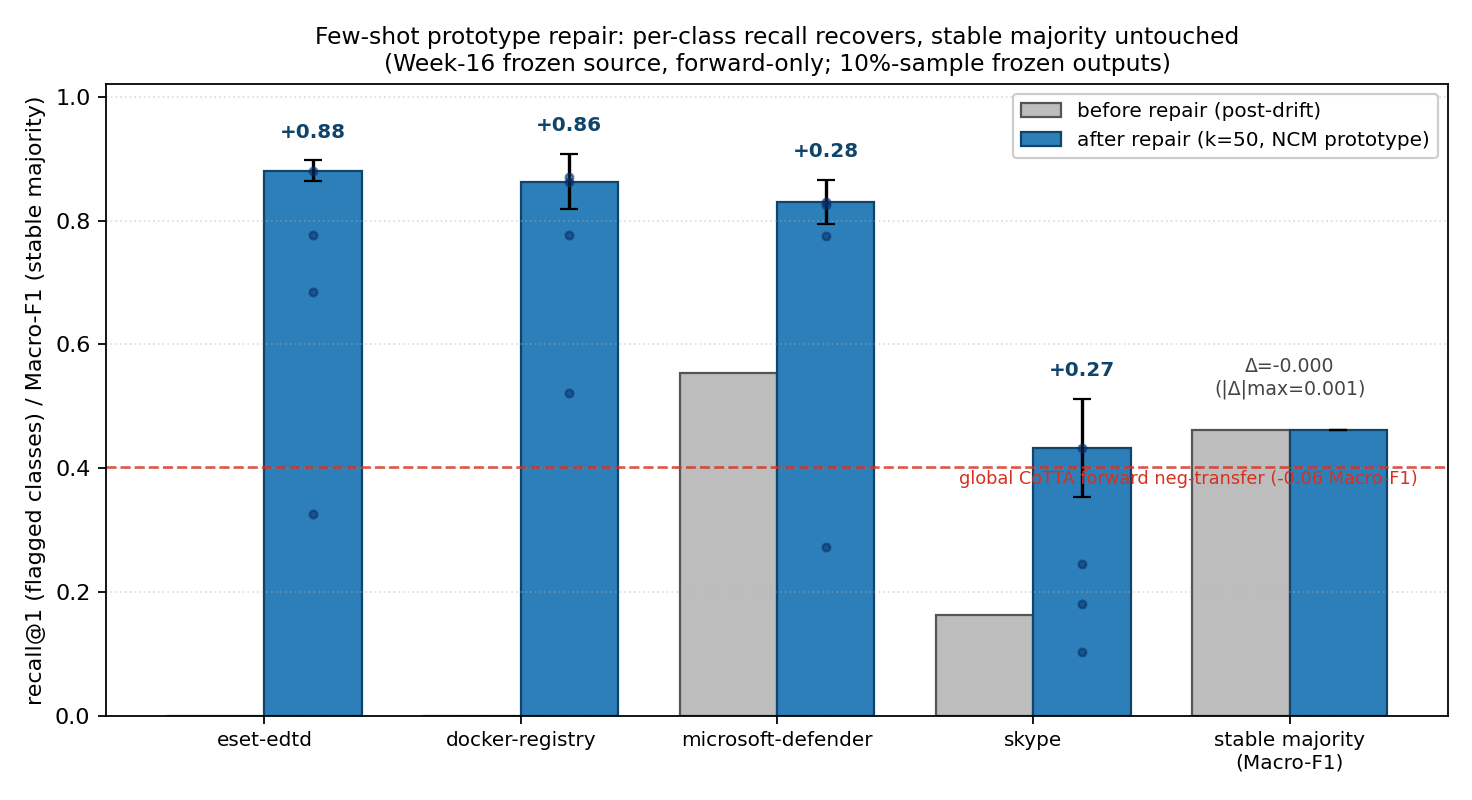
\includegraphics[width=\columnwidth]{figs/fig_perclass_before_after_w16.png}}
\caption{Per-class diagnose-and-repair (Week-16, frozen features). Recomputing
\emph{only} the flagged class's nearest-class-mean prototype from a $k$-shot
post-drift support set recovers per-class recall@1 on the teleported classes
(eset-edtd $0\to0.88$, docker-registry $0\to0.86$, skype $0.16\to0.43$ at $k{=}50$;
the non-teleported control microsoft-defender also rises $0.55\to0.83$) while the
stable-majority Macro-$F_1$ stays flat ($|\Delta|\leq0.001$), unlike CoTTA's
$-0.06$ negative transfer.}
\label{fig:repair}
\end{figure}

%==============================================================================
\section{Conclusion and Future Work}
\label{sec:conclusion}
We have argued, and shown, that the smooth accuracy decay of an encrypted-traffic
classifier is an illusion. Drift in this setting is discrete and per-class: the
macroscopic curve is a documented measurement-sensor step plus a long tail of
asynchronous per-class teleportations, not a continuous global shift. Because the
shift is local, the continuity assumption that UDA and CTTA rely on is
mis-specified here, and global adaptation is actively harmful --- gradient methods
induce negative transfer and even best-case adversarial alignment buys no forward
benefit, while the no-gradient AdaBN control does no harm, pinning the damage on
global parameter updates.

Our contribution is a robustness one. The BBSE-corrected entropy residual is a
noise-canceling tripwire: it preserves accurate, label-free tracking of hidden
$F_1$ (the clean-regime correlation reaches $\rho=-0.988$, which we present as
evidence of preserved tracking rather than as the headline result) while sharply
cutting false alarms under benign viral volume spikes (from 25.0\% to 4.6\% at
95\% detection on the Week-1 stream, with the ordering reproduced within the clean
Week-16 regime). Its two-sided mechanism --- robust to label shift, responsive to
covariate shift --- lets it localize \emph{which} application broke without any
labels, and our diagnose-and-repair demonstration shows that flag is actionable:
a per-class prototype recapture restores broken classes without disturbing the
stable majority.

Three directions remain open. First, stronger or doubly-robust estimators may
widen the robustness margin further
\cite{azizzadenesheli2019rlls,garg2020mlls,alexandari2020mlls,lee2023doubly,ziegler2023bayesian}.
Second, a full per-class few-shot class-incremental repair system, beyond the
frozen-feature proof of concept reported here, is the natural follow-up
\cite{rebuffi2017icarl,kirkpatrick2017ewc,li2017lwf,tao2020fscil}. Third, the
online setting is the mirror image of online label shift: where those methods
correct a drifting $P(y)$ under fixed $P(x\mid y)$, we cancel $P(y)$ and act
precisely when $P(x\mid y)$ breaks \cite{bai2022online,baby2023online}.

%==============================================================================
%  BIBLIOGRAPHY (carried over, verified). "% VERIFY" = not re-verified.
%
%  DO NOT RE-ADD (cut as off-topic / low-credibility):
%    - "Key Technologies for AI-Driven..." (Jianchao, n.d.)
%    - Mohanty (ABC + Genetic Algorithm + CNN)
%    - HyperPath-SVM ; IPSeg ; "Exemplar-Free CIL for Traffic Sign Classification"
%  DEFERRED (only if online-label-shift discussion expands): Dai et al. (CVPR'25);
%    Qian et al. (ICDM'23).
%==============================================================================
\begin{thebibliography}{00}

% --- Dataset & backbone -----------------------------------------------------
\bibitem{hynek2024cesnet} K. Hynek, J. Luxemburk, J. Pe\v{s}ek, T. \v{C}ejka, and P. \v{S}i\v{s}ka, ``CESNET-TLS-Year22: A year-spanning TLS network traffic dataset from backbone lines,'' \textit{Scientific Data}, vol.~11, art.~1156, 2024.
\bibitem{luxemburk2023tls} J. Luxemburk and T. \v{C}ejka, ``Fine-grained TLS services classification with reject option,'' \textit{Computer Networks}, vol.~220, art.~109467, 2023.
\bibitem{lin2022etbert} X. Lin, G. Xiong, G. Gou, Z. Li, J. Shi, and J. Yu, ``ET-BERT: A contextualized datagram representation with pre-training transformers for encrypted traffic classification,'' \textit{Proc. WWW}, 2022. % VERIFY
\bibitem{shamsimukhametov2024ech} D. Shamsimukhametov, A. Kurapov, M. Liubogoshchev, and E. M. Khorov, ``Early traffic classification with Encrypted ClientHello: A multi-country study,'' \textit{IEEE Access}, vol.~12, pp.~142979--142993, 2024.

% --- Failure modes / drift in ETC -------------------------------------------
\bibitem{malekghaini2022data} N. Malekghaini et al., ``Data drift in DL: lessons learned from encrypted traffic classification,'' \textit{IFIP Networking Conf.}, pp.~1--9, 2022.
\bibitem{chen2025drift} Z. Chen et al., ``Drift-oriented self-evolving encrypted traffic application classification for actual network environment,'' \textit{arXiv:2501.04246}, 2025.
\bibitem{seddigh2019framework} N. Seddigh et al., ``A framework \& system for classification of encrypted network traffic using machine learning,'' \textit{15th CNSM}, pp.~1--5, 2019.
\bibitem{jancicka2024noms} L. Jan\v{c}i\v{c}ka et al., ``Analysis of statistical distribution changes of input features in the network traffic classification domain,'' \textit{IEEE/IFIP NOMS}, 2024. % confirm full co-authors
\bibitem{pendlebury2019tesseract} F. Pendlebury, F. Pierazzi, R. Jordaney, J. Kinder, and L. Cavallaro, ``TESSERACT: Eliminating experimental bias in malware classification across space and time,'' \textit{USENIX Security}, 2019. % VERIFY

% --- TTA / UDA canon --------------------------------------------------------
\bibitem{wang2020tent} D. Wang, E. Shelhamer, S. Liu, B. Olshausen, and T. Darrell, ``Tent: Fully test-time adaptation by entropy minimization,'' \textit{ICLR}, 2021.
\bibitem{wang2022cotta} Q. Wang, O. Fink, L. Van Gool, and D. Dai, ``Continual test-time domain adaptation,'' \textit{CVPR}, 2022.
\bibitem{ganin2016dann} Y. Ganin et al., ``Domain-adversarial training of neural networks,'' \textit{J. Mach. Learn. Res.}, vol.~17, pp.~1--35, 2016.
\bibitem{li2016adabn} Y. Li, N. Wang, J. Shi, J. Liu, and X. Hou, ``Revisiting batch normalization for practical domain adaptation (AdaBN),'' \textit{arXiv:1603.04779} / ICLR Workshop, 2017. % VERIFY (venue/year)

% --- Datasets: secondary (QUIC) ---------------------------------------------
\bibitem{luxemburk2023quic} J. Luxemburk, K. Hynek, T. \v{C}ejka, A. Luka\v{c}ovi\v{c}, and P. \v{S}i\v{s}ka, ``CESNET-QUIC22: A large one-month QUIC network traffic dataset from backbone lines,'' \textit{Data in Brief}, art.~108888, 2023.

% --- Unsupervised drift monitoring (closest prior art) ----------------------
\bibitem{mfwdd2024} L. Jan\v{c}i\v{c}ka, D. Soukup, J. Koumar, F. N\v{e}mec, and T. \v{C}ejka, ``MFWDD: Model-based feature weight drift detection showcased on TLS and QUIC traffic,'' \textit{20th Int. Conf. Network and Service Management (CNSM)}, 2024.
\bibitem{cesnetdrift2025} CESNET, ``A drift-based dataset stability benchmark for encrypted traffic classification,'' \textit{arXiv:2512.23762}, 2025. % confirm authors/exact title

% --- Adjacent encrypted-traffic analysis: drift & per-class handling --------
%     (WF + mobile-app fingerprinting; added from the related literature.
%      Bibliographic details taken from the source PDFs -- confirm page ranges /
%      venue strings against the official versions before camera-ready.)
\bibitem{deng2023ares} X. Deng, Q. Yin, Z. Liu, X. Zhao, Q. Li, M. Xu, K. Xu, and J. Wu, ``Robust multi-tab website fingerprinting attacks in the wild,'' in \textit{IEEE Symposium on Security and Privacy (SP)}, 2023, pp.~1005--1022.
\bibitem{deng2024holmes} X. Deng, Q. Li, and K. Xu, ``Robust and reliable early-stage website fingerprinting attacks via spatial-temporal distribution analysis,'' in \textit{Proc. ACM SIGSAC Conf. on Computer and Communications Security (CCS)}, 2024. % confirm page range
\bibitem{bahramali2023netclr} A. Bahramali, A. Bozorgi, and A. Houmansadr, ``Realistic website fingerprinting by augmenting network traces,'' in \textit{Proc. ACM SIGSAC Conf. on Computer and Communications Security (CCS)}, 2023, pp.~1035--1049.
\bibitem{jiang2022fgnet} M. Jiang, Z. Li, P. Fu, W. Cai, M. Cui, G. Xiong, and G. Gou, ``Accurate mobile-app fingerprinting using flow-level relationship with graph neural networks,'' \textit{Computer Networks}, vol.~217, art.~109309, 2022.
% OPTIONAL -- marginal to this thesis (in-kernel IDS + NN quantization; CIC-IDS,
% not a drift study). Enable + cite ONLY if the few-shot / parameter hot-update
% repair angle in Sec.~\ref{sec:operational} is expanded:
% \bibitem{zhang2024nnebpf} J. Zhang, P. Chen, Z. He, H. Chen, and X. Li, ``Real-time intrusion detection and prevention with neural network in kernel using eBPF,'' in \textit{IEEE/IFIP Int. Conf. on Dependable Systems and Networks (DSN)}, 2024, pp.~416--428.

% --- Label-shift quantification (the math we weaponize) ---------------------
\bibitem{lipton2018bbse} Z. Lipton, Y.-X. Wang, and A. Smola, ``Detecting and correcting for label shift with black box predictors,'' \textit{ICML}, 2018.
\bibitem{saerens2002sld} M. Saerens, P. Latinne, and C. Decaestecker, ``Adjusting the outputs of a classifier to new a priori probabilities: a simple procedure,'' \textit{Neural Computation}, vol.~14, no.~1, pp.~21--41, 2002.
\bibitem{azizzadenesheli2019rlls} K. Azizzadenesheli, A. Liu, F. Yang, and A. Anandkumar, ``Regularized learning for domain adaptation under label shifts,'' \textit{ICLR}, 2019. % VERIFY
\bibitem{garg2020mlls} S. Garg, Y. Wu, S. Balakrishnan, and Z. Lipton, ``A unified view of label shift estimation,'' \textit{NeurIPS}, 2020. % VERIFY
\bibitem{ziegler2023bayesian} A. Ziegler and P. Czy\.{z}, ``Bayesian quantification with black-box estimators,'' \textit{Transactions on Machine Learning Research (TMLR)}, 2023. % VERIFY

% --- Online label shift (CONTRAST + future work only) -----------------------
\bibitem{bai2022online} Y. Bai, Y.-J. Zhang, P. Zhao, M. Sugiyama, and Z.-H. Zhou, ``Adapting to online label shift with provable guarantees,'' \textit{NeurIPS}, vol.~35, pp.~29960--29974, 2022.
\bibitem{baby2023online} D. Baby, S. Garg, T.-C. Yen, S. Balakrishnan, Z. C. Lipton, and Y.-X. Wang, ``Online label shift: optimal dynamic regret meets practical algorithms,'' \textit{NeurIPS}, vol.~36, pp.~65703--65742, 2023.

% --- Advanced estimator for FUTURE WORK ONLY --------------------------------
\bibitem{lee2023doubly} J. Lee, Y. Ma, and H. Zhao, ``Doubly flexible estimation under label shift,'' \textit{J. American Statistical Association}, vol.~120, no.~549, 2024 (arXiv:2307.04250). % cite ONLY in future work.

% --- Attribution ------------------------------------------------------------
\bibitem{lundberg2017shap} S. M. Lundberg and S.-I. Lee, ``A unified approach to interpreting model predictions,'' \textit{NeurIPS}, 2017. % VERIFY

% --- Open-set + continual learning (operational paradigm) -------------------
\bibitem{bendale2016openmax} A. Bendale and T. E. Boult, ``Towards open set deep networks,'' \textit{CVPR}, 2016. % VERIFY
\bibitem{rebuffi2017icarl} S.-A. Rebuffi, A. Kolesnikov, G. Sperl, and C. H. Lampert, ``iCaRL: Incremental classifier and representation learning,'' \textit{CVPR}, 2017. % VERIFY
\bibitem{kirkpatrick2017ewc} J. Kirkpatrick et al., ``Overcoming catastrophic forgetting in neural networks,'' \textit{PNAS}, vol.~114, no.~13, pp.~3521--3526, 2017. % VERIFY
\bibitem{li2017lwf} Z. Li and D. Hoiem, ``Learning without forgetting,'' \textit{IEEE TPAMI}, 2017. % VERIFY
\bibitem{tao2020fscil} X. Tao, X. Hong, X. Chang, S. Dong, X. Wei, and Y. Gong, ``Few-shot class-incremental learning,'' \textit{CVPR}, 2020. % VERIFY
\bibitem{alexandari2020mlls} A. Alexandari, A. Kundaje, and A. Shrikumar, ``Maximum likelihood with bias-corrected calibration is hard-to-beat at label shift adaptation,'' \textit{ICML}, 2020.
\bibitem{shahraki2022active} A. Shahraki et al., ``Active learning for network traffic classification: a technical survey,'' \textit{IEEE Transactions on Cognitive Communications and Networking}, 2022.

\end{thebibliography}

%==============================================================================
%  APPENDIX — FIGURES NOT USED IN THE BODY (for the advisor discussion)
%  ------------------------------------------------------------------
%  Left OUT of the body (or moved here). Listed so we can decide together what to
%  pull back in. All paths flat (figs/<name>.png).
%  NOTE: fig_mirror_extreme_fwd_* are NOT here -- they are the symmetric CONTROL
%        in Sec.~\ref{sec:robustness} (Fig.~\ref{fig:symmetric}).
%==============================================================================
\appendix
\section*{Appendix: Figures Considered but Not Used}

This appendix collects supporting and parked figures: the Week-1 mirror that
tracks through the documented Week-10 event, the contamination-separability panel
referenced in-text in Sec.~\ref{sec:isolation}, the external-validation
teleportation on the proprietary closed-world dataset (pending disclosure
clearance), and assets superseded by their Week-16 equivalents in the body.

\begin{figure}[htbp]
\centerline{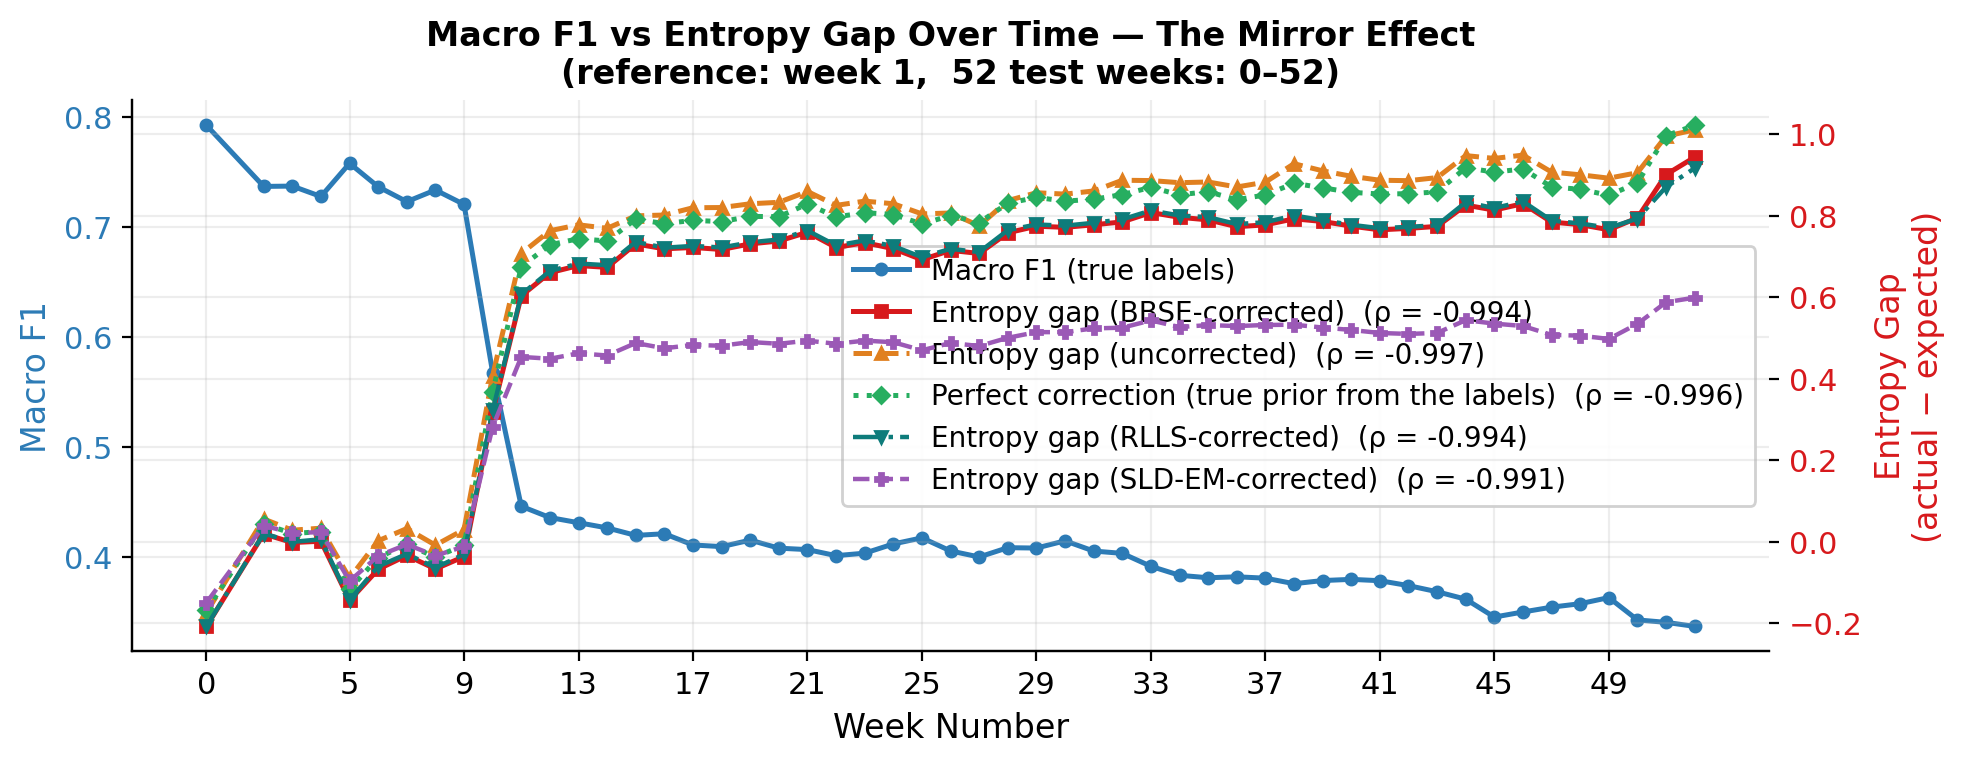
\includegraphics[width=\columnwidth]{figs/fig_mirror_effect (1).png}}
\caption{Week-1 Mirror Effect (supplementary): clean tracking
$\rho=-0.997$ (uncorr.) / $-0.994$ (BBSE), spanning the documented Week-10 event.
Superseded as primary by the Week-16 forward mirror (Fig.~\ref{fig:mirror});
retained here because it shows tracking THROUGH the Week-10 covariate event.}
\label{fig:app_mirror_w1}
\end{figure}

\begin{figure}[htbp]
% EXTERNAL VALIDATION on an anonymized closed-world dataset. Toggle ON once
% (i) disclosure is permitted and (ii) it does not deanonymize us under
% double-blind. Until then keep the includegraphics commented to avoid a
% compile error (file not yet on disk).
% \centerline{\includegraphics[width=\columnwidth]{figs/fig_tsne_closedworld_anon.png}}
\centerline{\fbox{\parbox{0.9\columnwidth}{\centering\vspace{1em}
\textit{[t-SNE teleportation on the proprietary closed-world dataset --- figure
pending disclosure/anonymity clearance.]}\vspace{1em}}}}
\caption{External validation (pending clearance). The same per-class
``teleportation'' on an independent, closed-world proprietary dataset
(anonymized for review), establishing that teleportation is not a CESNET
artifact. Referenced from Sec.~\ref{sec:modalities} and Sec.~\ref{sec:negtransfer}.
\TODO{toggle on once disclosure/anonymity is cleared.}}
\label{fig:app_proprietary_tsne}
\end{figure}

\begin{figure}[htbp]
\centerline{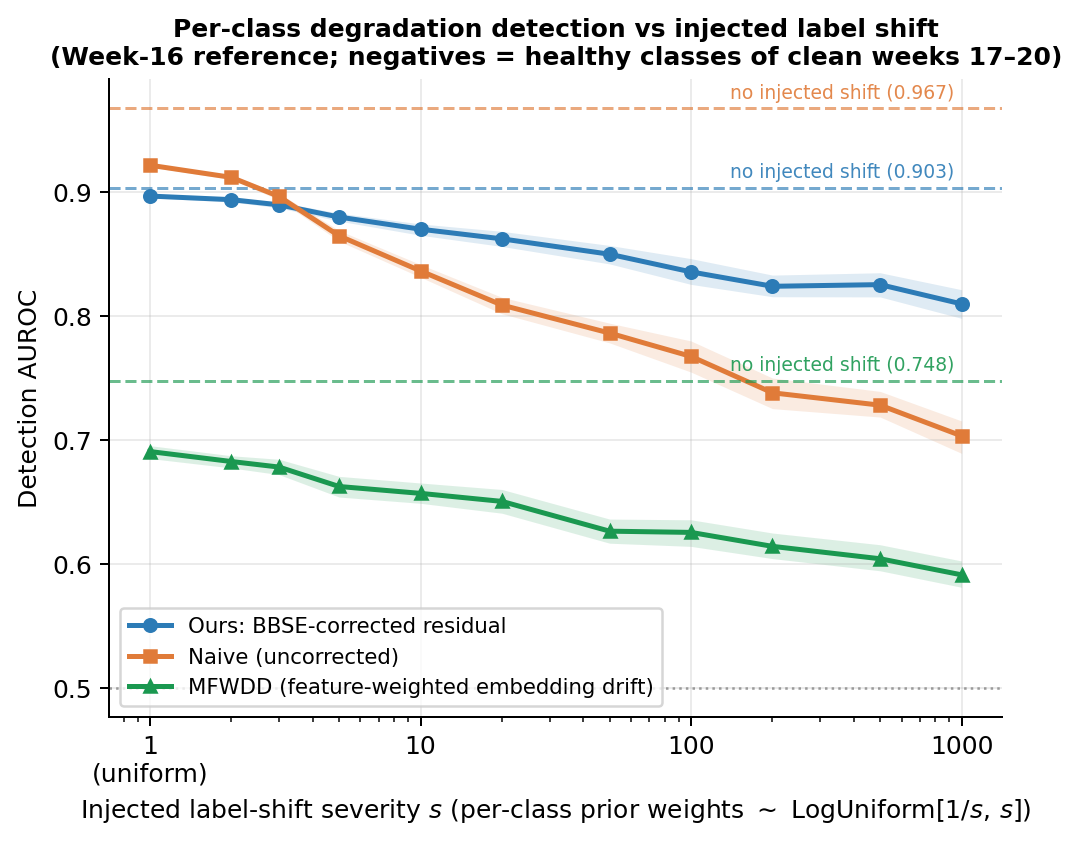
\includegraphics[width=\columnwidth]{figs/fig_isolation_auroc_vs_labelshift_fwd.png}}
\caption{Supplementary: 3-detector (ours / naive / MFWDD) detection AUROC vs label
shift, forward (Week-16). The body presents the fuller estimator-variant sweep
(Fig.~\ref{fig:sweep}).}
\label{fig:app_3det_fwd}
\end{figure}

\begin{figure}[htbp]
\centerline{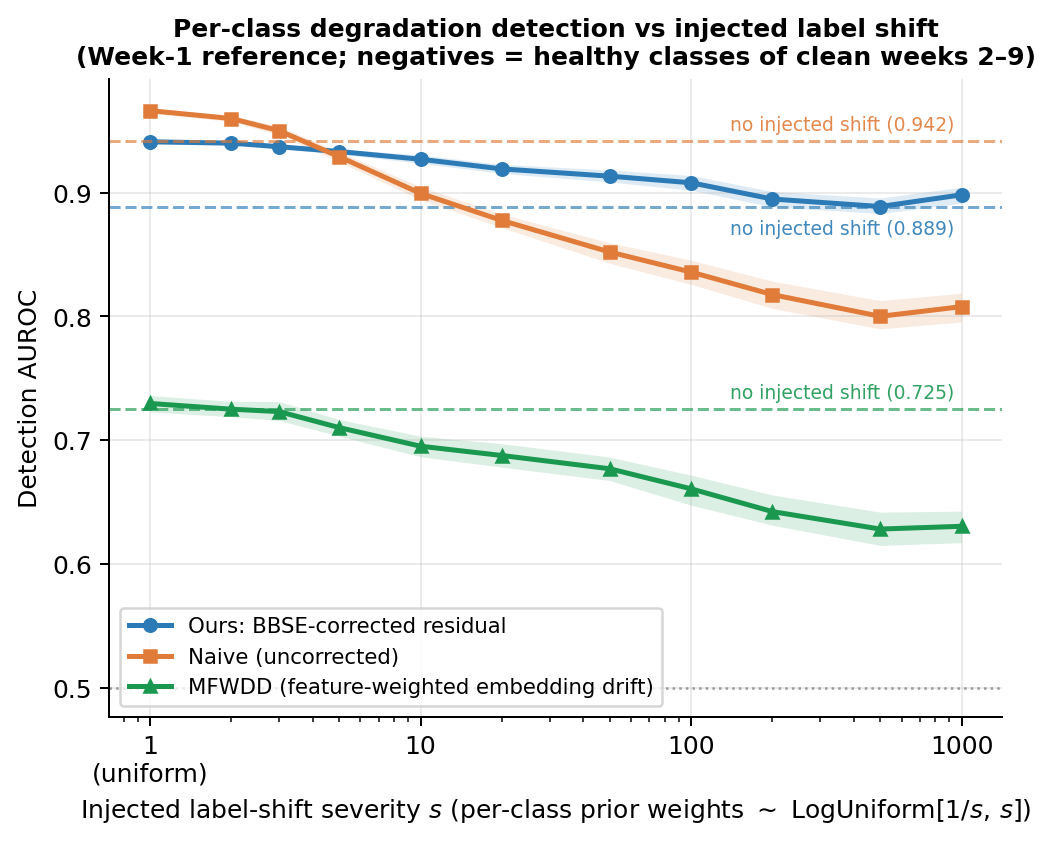
\includegraphics[width=\columnwidth]{figs/fig_isolation_auroc_vs_labelshift.png}}
\caption{Supplementary: the same 3-detector AUROC-vs-shift over the weeks 13--20
window (companion to Fig.~\ref{fig:app_3det_fwd}).}
\label{fig:app_3det_1320}
\end{figure}

\begin{figure}[htbp]
\centerline{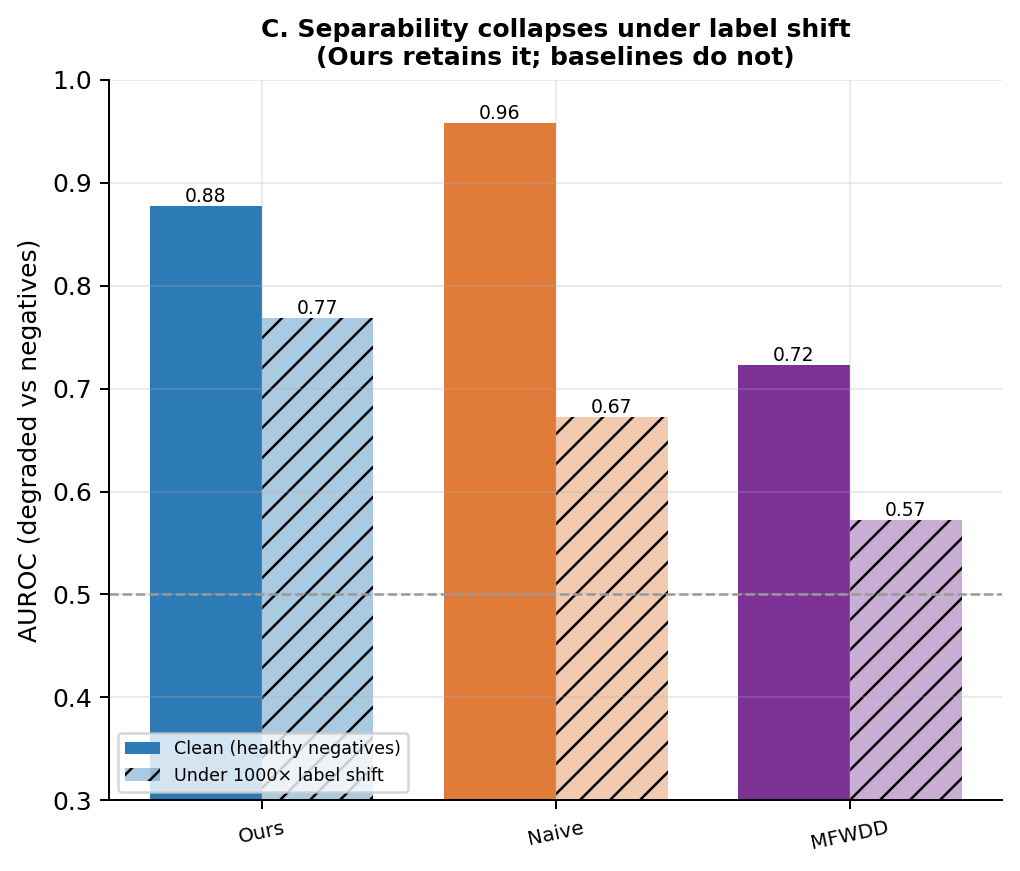
\includegraphics[width=\columnwidth]{figs/fig_isolation_C_auroc_contamination_fwd.png}}
\caption{Panel C (Week-16 forward), reported in-text in Sec.~\ref{sec:isolation}:
separability under 1000x contamination --- ours degrades least
(0.88$\to$0.77) and overtakes uncorrected, which collapses (0.96$\to$0.67); MFWDD
0.72$\to$0.57.}
\label{fig:app_panelC}
\end{figure}

\begin{figure}[htbp]
\centerline{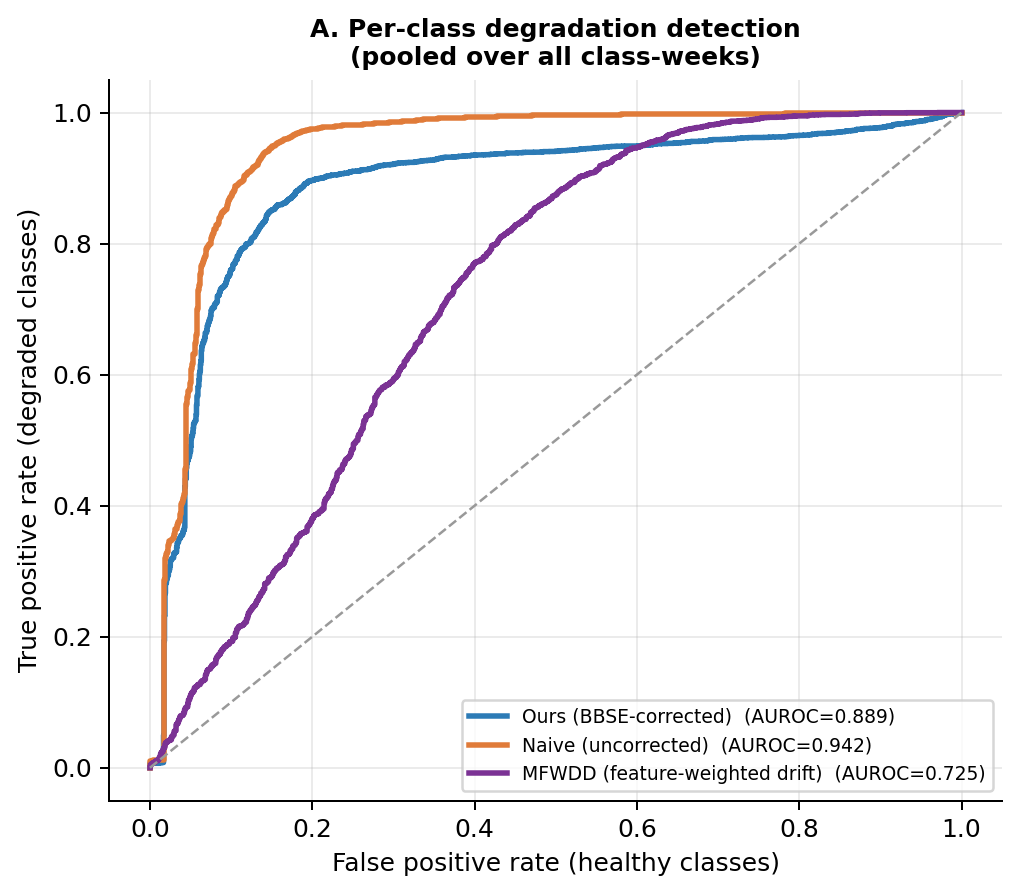
\includegraphics[width=\columnwidth]{figs/fig_isolation_A_roc_detection.png}}
\caption{Supplementary (Week-1 reference): the original Week-1 isolation ROC panel,
kept for reference-sensitivity comparison; the body uses the Week-16 version
(Fig.~\ref{fig:isopanels}).}
\label{fig:app_iso_w1}
\end{figure}

%  NON-FIGURE asset to raise with advisor:
%  - The third, proprietary closed-world dataset (anonymized) negative-transfer
%    results reproduce the effect MORE strongly. Out of body; bring rows/sentence
%    in ONLY if disclosure permitted and it does not deanonymize us -- and keep it
%    consistent with the t-SNE above (both in, or both out).
%  - OPTIONAL per-week macro-decay curve (commented near Sec.~\ref{sec:intro}).

\end{document}